\documentclass[twoside,english]{uiofysmaster}
%\bibliography{references}

\usepackage{array}
\usepackage{booktabs}
\usepackage{float}
\usepackage{scrextend}
\usepackage{amsfonts}
\usepackage{amsmath,amsfonts,amssymb}
\addtokomafont{labelinglabel}{\sffamily}

\usepackage[boxed]{algorithm2e}

% For identity matrix
%\usepackage{dsfont}

% To show code
\usepackage{listings}

% Feynman diagrams
\usepackage[compat=1.1.0]{tikz-feynman}
\usepackage{tikz}

% Allow verbatim in footnotes
\usepackage{bigfoot}

\setlength{\heavyrulewidth}{1.5pt}
\setlength{\abovetopsep}{4pt}

\usepackage[boxed]{algorithm2e}
\addtokomafont{labelinglabel}{\sffamily}

% Multicolumns for calculation
%\usepackage{multicol}

% Subfigures
\usepackage{subcaption}
\usepackage{sidecap}

% For quotes
\usepackage[autostyle]{csquotes} 

% For appendices
\usepackage[toc,page]{appendix}


% For independence symbol
\usepackage{graphicx}

\newcommand{\bigCI}{\mathrel{\text{\scalebox{1.07}{$\perp\mkern-10mu\perp$}}}}




\usepackage{slashed}
\begin{document}


\title{Gaussian Processes for Supersymmetry}
\author{Ingrid Holm}
\date{May 2018}

\maketitle

\begin{abstract}
This is an abstract text.
\end{abstract}

\begin{dedication}
  To someone
  \\\vspace{12pt}
  This is a dedication to my cat.
\end{dedication}

\begin{acknowledgements}
  I acknowledge my acknowledgements.
\end{acknowledgements}

\tableofcontents


\chapter{Introduction}

- why nlo?

- why gp?

- why dgp?

\chapter{Physics Background}



This chapter is about supersymmetry. Familiarity with quantum field theory, the Standard Model of particle physics and some group theory is assumed. The Higgs mechanism and the hierarchy problem are reviewed, before supersymmetry is outlined. Finally, the Minimal Supersymmetric Standard Model is introduced, with its corresponding field content.

\section{The Standard Model}

The Standard Model of particle physics has successfully explained almost all experimental results and predicted several phenomena in particle physics. One of the main attributes of this model is that particles with different values of the \textit{spin} quantum number behave differently. Particles with half-integer and integer spin values are called \textit{fermions} and \textit{bosons}, respectively. Fermions are particles such as quarks and leptons, which interact through the exchange of bosons. The Standard Model bosons are the \textit{photon} (electromagnetic interaction), the \textit{gluon} (strong interaction that holds atoms together), the $W$ and $Z$ bosons (the weak interaction) and the famously elusive \textit{Higgs boson}. The equations of motion and allowed interactions can all be derived from the \textit{Lagrangian} of the Standard Model. The Lagrangian, of which the time integral is the action $S$, is invariant to transformations under the Lorentz group --- or a change of reference frame in the language of special relativity. 

\subsubsection{The Higgs Mechanism}

The Standard Model is a gauge theory based on the symmetry group $SU(3)_C \times SU(2)_L \times U(1)_Y$. The $SU(3)$ group is the symmetry group for strong interactions, or quantum chromodynamics, and $SU(2)_L \times U(1)_Y$ is the electroweak symmetry group. In order for the particles to obtain masses the electroweak symmetry must be spontaneously broken down to $U(1)_{em}$. The symmetry is broken when the Higgs field obtains a non-zero \textit{vacuum expectation value} (vev) --- meaning that it has some field value when the governing potential is at its minimum. The Higgs field $\Phi$ is a self-interacting complex $SU(2)_L$ doublet whose Lagrangian is given by
\begin{align}
\mathcal{L}_{\Phi} = \partial_{\mu} \Phi^{\dagger} \partial^{\mu} \Phi + V(\Phi),
\end{align}
where the first term is the kinetic term, and the scalar potential describing the Higgs $V(\Phi)$ is the famous Mexican hat potential
\begin{align}
V(\Phi) = \mu^2 \Phi^{\dagger} \Phi + \lambda (\Phi^{\dagger} \Phi)^2.
\end{align}
For $\mu^2 < 0$ and $\lambda > 0$ this potential aquires a non-trivial minimum given by
\begin{align}
|\Phi_0| = \sqrt{\frac{-\mu^2}{2\lambda}} \equiv \frac{v}{\sqrt{2}},
\end{align}
where $v$ is the vacuum expectation value. A special parameterization of the Higgs $SU(2)_L$ doublet, $\Phi^T(x) = \frac{1}{\sqrt{2}} (0, v + h(x))$, leads to the Lagrangian developing mass terms for fermions and the gauge bosons $Z$ and $W^{\pm}$. The mass terms are proportional to $v$, \textit{e.g.}
\begin{align*}
M_W = \frac{1}{2} v g,
\end{align*}
where $M_W$ is the mass of the $W$ and $g$ is the $SU(2)_L$-coupling. The Higgs' own mass provides one of the strongest arguments for introducing supersymmetry, namely the \textit{hierarchy problem}, which is discussed below. 

Another argument for the introduction of supersymmetry is gauge coupling unification. Gauge coupling unification is the assumption that the Standard Model symmetry group is a unified gauge group, \textit{e.g.} $SU(5)$ or $SO(10)$, broken down to $SU(3)_C \times SU(2)_L \times U(1)_Y$ at some high energy scale. However, this is not discussed in this thesis.

\section{The Hierarchy Problem}

The Higgs boson was discovered at the LHC in 2012, and its mass  measured at $m_H \sim 125$ GeV \cite{20121}. The expression for the Higgs mass in the Standard Model includes loop corrections, which provide a large discrepancy between theory and experiment. The Higgs mass receives fermionic or scalar loop-contributions to its mass such as those shown in Fig. (\ref{Fig:: Phys. bac.: Higgs mass contributions}). The expression for the mass can thus be written in terms of the bare parameter $m_{H0}$ and the corrections $\Delta m_H$
\begin{align*}
m_H^2 = m_{H0}^2 + \Delta m_H^2.
\end{align*}
Loop diagrams contain divergences, because of integrals over all possible momenta for the virtual particles in the loops. A way to get rid of these infinities is to regularize the expressions. Regularization is a neat trick that introduces a \textit{cut-off scale}, which sets an upper limit on the momentum that is integrated over. A common choice for the cut-off scale $\Lambda$ is the Planck scale, as this is where new physics is needed to explain gravity in the Standard Model. The Planck scale is of the order of $\Lambda_{UV} \sim 10^{18}$ GeV. After regularization, the mass correction terms are
\begin{align}
\Delta m_H^2 = - \frac{|\lambda_f|^2}{8\pi^2} \Lambda_{UV}^2 + \frac{\lambda_s}{16\pi^2} \Lambda_{UV}^2 +...,
\end{align}
where $\lambda_s$ is the coupling of the Higgs to the scalar, and $\lambda_f$ is the Higgs coupling to the fermion. The problem now becomes apparent: the correction to the mass is proportional to the Planck scale, placing it at the order of $10^{18}$ Gev, yet the mass has been experimentally measured around $125$ GeV. There must be some colossal cancellation of terms with a tremendous tuning of the SM parameters in $\lambda_s$ and $\lambda_f^2$. Tuning of parameters is undesirable --- the model should be as natural as possible. 

\begin{figure}[H]
\centering
\includegraphics[scale=0.3]{figures_physical_background/hierarchy_problem.png}
\caption{Fermion and scalar one-loop corrections to the Higgs mass. Figure from \cite{batzing2017lecture}.}
\label{Fig:: Phys. bac.: Higgs mass contributions}
\end{figure}

Supersymmetry provides an elegant solution to the hierarchy problem. In simple terms, supersymmetry introduces a fermionic superpartner for each boson, and vice versa. These are called sparticles, and have a prefix -s for the partners of fermions, such as \textit{squarks} and \textit{leptons}, and the suffix -ino for partners of bosons, such as the \textit{photino} and \textit{Higgsino}. In unbroken supersymmetry these particles have identical mass, and their couplings to the Higgs are the same $\lambda_s = |\lambda_f|^2$. In addition, there are twice as many scalars as fermions, which gives a perfect cancellation of these enormous corrections. Unbroken supersymmetry therefore solves the hierarchy problem. The case of broken supersymmetry is revisited in a later section.


\section{Supersymmetry}

Supersymmetry is an extension of symmetries. Relativistic field theories are invariant under boosts, rotations and translations in spacetime. These are called Poincar\'{e} transformations, and are given by
\begin{align}
x^{\mu} \rightarrow x'^{\mu} = \Lambda^{\mu}_{\ \nu} x^{\nu} + a^{\mu}, 
\end{align}
where $\Lambda^{\mu}_{\ \nu}$ is a Lorentz transformation and $a^{\mu}$ is a translation. The assumption behind supersymmetry is that Nature obeys a non-trivial extension of the related Poincar\'{e} algebra, namely the \textit{superalgebra}. 

The elements of the superalgebra and their representations can be described using \textit{superspace}. Coordinates in superspace are given by $z^{\pi} = (x^{\mu}, \theta^A, \bar{\theta}_{\dot{A}})$, where $x^{\mu}$ are the well-known Minkowski coordinates, and $\theta^A, \bar{\theta}_{\dot{A}}$ are four Grassmann numbers \footnote{Grassmann numbers are numbers that anti-commute.}. Any Super-Poincar\'{e} transformation can be written in the following way
\begin{align}
L(a, \alpha) = \exp [-i a^{\mu} P_{\mu} + i \alpha^A Q_A + i \bar{\alpha}^{\dot{A}} \bar{Q}_{\dot{A}} ].
\end{align}
In addition, since $P_{\mu}$ commutes with the generators $Q$ one can always boost between reference frames, so in general a supersymmetry transformation is taken to mean
\begin{align}
\delta_S = \alpha^A Q_A + \bar{\alpha}_{\dot{A}} \bar{Q}^{\bar{A}}.
\end{align}


The super-Poincar\'{e} algebra is given by the following commutation and anticommutation relations \cite{kvellestad2015chasing}
\begin{align}
\{Q_A, Q_B \} &= \{ \bar{Q}_A, \bar{Q}_B\} = 0,\\
\{Q_A, \bar{Q}_{\dot{A}} \} &= 2 (\sigma^{\mu})_{A \dot{A}} P_{\mu},\\
[Q_A, P^{\mu}] &= [\bar{Q}_A, P^{\mu}] = 0,\label{Eq:: [Q,P]}\\
[Q_A, M^{\mu \nu}] &= \frac{1}{2} (\sigma^{\mu \nu})_A^B Q_B,\\
[\bar{Q}_{\dot{A}}, M^{\mu \nu}] &= \frac{1}{2} (\bar{\sigma}^{\mu \nu})_{\dot{a}}^{\dot{b}} Q_{\dot{b}}^{\dagger},  
\end{align}
where $Q_A, A=1,2,3,4$ are the superalgebra generators, $P^{\mu}$ are the generators of translation, and $M^{\mu \nu}$ are the generators of the Lorentz group. 

The supersymmetry generators turn fermions into bosons and vice versa. More specifically, these operators have the following commutation relations with the rotation generator $J^3$
\begin{align}
[ Q_A, J^3] &= \frac{1}{2} (\sigma^3)_A^BQ_B, 
\end{align}
which for the $Q_1$ generator becomes
\begin{align}
[Q_1, J^3] = \frac{1}{2} Q_1.
\end{align}
Using this operator on a state in an irreducible representation of the Poincar\'{e} algebra with mass $m$ and spin $j_3$ gives
\begin{align}
J^3 Q_1 \ket{m, j_3} = (j_3 - \frac{1}{2}) Q_1 \ket{m, j_3},
\end{align}
thus lowering the spin of the state by $1/2$. Similarly, $Q_2$ would increase the spin. They do not, however, change the mass. This can be seen from Eq.\ (\ref{Eq:: [Q,P]})
\begin{align}
P^{\mu} P_{\mu} Q_A \ket{m, j_3} = Q_A P^{\mu} P_{\mu} \ket{m, j_3} = m^2 Q_A \ket{m, j_3}.
\end{align}
States that transform into each other via $Q_A$ and $\bar{Q}_{\dot{A}}$ are called \textit{superpartners}. In unbroken supersymmetry, therefore, the partnering fermions and bosons have the same mass. If this were the case, supersymmetric particles would already have been discovered, so supersymmetry must be a broken symmetry.
% These generators can be written as 
%\begin{align}
%P_{\mu} &= i \partial_{\mu},\\
%iQ_A &= -i (\sigma^{\mu} \bar{\theta})_A \partial_{\mu} + %\partial_A,\\
%i \bar{Q}^{\dot{A}} &= -i (\bar{\sigma}^{\mu} \theta)^{\dot{A}} \partial_{\mu} + \partial^{\dot{A}}.
%\end{align}
\subsection{Superfields}

A supersymmetric Lagrangian will need a derivative that is invariant under supersymmetry transformations. The general covariant derivatives are defined as
\begin{align}
D_A & \equiv \partial_A + i (\sigma^{\mu} \bar{\theta})_A \partial_{\mu},\\
\bar{D}^{\dot{A}} & \equiv -\partial^{\dot{A}} - i (\sigma^{\mu} \theta)^{\dot{A}} \partial_{\mu}.
\end{align}

The covariant derivatives work on the \textit{superfields} $\Phi$, which are functions on superspace $\Phi(x, \theta, \bar{\theta})$. These are affected by the covariant derivatives in the following way
\begin{align}
\bar{D}_{\dot{A}} \Phi (x, \theta, \bar{\theta}) &= 0 &\text{(left-handed scalar superfield)},\\
D^A \Phi^{\dagger} (x, \theta, \bar{\theta}) &= 0 &\text{(right-handed scalar superfield)}\\
\end{align}
The fields $\Phi$ are required to be Lorentz scalars or pseudoscalars, which restricts the properties of their component fields. It can be shown that the left- and right-handed scalar fields can be written in terms of their component fields as  \cite{batzing2017lecture}
\begin{align}
\Phi (x, \theta, \bar{\theta}) =& A(x) + i (\theta \sigma^{\mu} \bar{\theta}) \partial_{\mu} A(x) - \frac{1}{4} \theta \theta \bar{\theta} \bar{\theta} \Box A(x) + \sqrt{2} \theta \psi (x)\nonumber \\ 
& - \frac{i}{\sqrt{2}} \theta \theta \partial_{\mu} \psi (x) \sigma^{\mu} \bar{\theta} + \theta \theta F(x),\\
\Phi^{\dagger} (x, \theta, \bar{\theta}) =& A^*(x) - i (\theta \sigma^{\mu} \bar{\theta}) \partial_{\mu} A^*(x) - \frac{1}{4} \theta \theta \bar{\theta} \bar{\theta} \Box A^*(x) + \sqrt{2} \bar{\theta} \bar{\psi} (x)\nonumber \\
& - \frac{i}{\sqrt{2}} \bar{\theta} \bar{\theta} \theta \sigma^{\mu} \partial_{\mu} \bar{\psi} (x)  + \bar{\theta} \bar{\theta} F^*(x),
\end{align}
where $A(x)$ and $F(x)$ are complex scalars and $\psi_A(x)$ and $\bar{\psi}^{\dot{A}} (x)$ are left-handed and right-handed Weyl spinors, respectively. 

A vector field is defined by the constraint
\begin{align}
\Phi (x, \theta, \bar{\theta}) &= \Phi^{\dagger} (x, \theta, \bar{\theta}).\label{Eq:: vector field}
\end{align}
From Eq.\ (\ref{Eq:: vector field}) the structure of a general vector field should be  \cite{batzing2017lecture}
\begin{align}
\Phi (x, \theta, \bar{\theta}) =& f(x) + \theta \varphi (x) + \bar{\theta} \bar{\varphi} (x) + \theta \theta m(x) + \bar{\theta} \bar{\theta} m^* (x) \nonumber \\
&+ \theta \sigma^{\mu} \bar{\theta} V_{\mu} (x) + \theta \theta \bar{\theta} \bar{\lambda} (x) + \bar{\theta} \bar{\theta} \theta \lambda (x) + \theta \theta \bar{\theta} \bar{\theta} d(x),
\end{align}
where $f(x)$, $d(x)$ are real scalar fields, $\varphi_A (x)$, $\lambda_A (x)$ are Weyl spinors, $m(x)$ is a complex scalar field and $V_{\mu} (x)$ is a real Lorentz four-vector. An example of a vector field is the product $V = \Phi^{\dagger} \Phi$. In the $j = \frac{1}{2}$ representation of the superalgebra, this field does not correspond to the promised number of degrees of freedom. This problem is fixed by the super-gauge. 



\subsection{Supersymmetric Lagrangian}

Symmetry transformations of the Lagrangian should leave the action
\begin{align}
S \equiv \int d^4x \mathcal{L},
\end{align}
 invariant. This is automatically fulfilled if the Lagrangian only changes by a total derivative. It can be shown that the highest order component fields in $\theta$ and $\bar{\theta}$ of the scalar and vector superfields have this property. To ensure that the action is invariant under supersymmetry transformations, the Lagrangian is redefined such that
\begin{align}
S = \int d^4x \int d^4 \theta \mathcal{L},
\end{align}
where there is now an integral over Grassmann numbers and $d^4 \theta = d^2 \theta d^2 \bar{\theta}$.

Restrictions on the supersymmetric Lagrangian, such as invariance under supersymmetric transformations and renormalizability, mean that the most general Lagrangian as a function of the scalar superfields $\Phi_i$ is
\begin{align}
\mathcal{L} = \Phi_i^{\dagger} \Phi_i + \bar{\theta} \bar{\theta} W[\Phi] + \theta \theta W[\Phi^{\dagger}],
\end{align}
where $\Phi_i^{\dagger} \Phi_i$ is the kinetic term, and $W[\Phi]$ is the \textit{superpotential}
\begin{align}\label{Eq:: superpotential}
W[\Phi] = g_i \Phi_i + m_{ij} \Phi_i \Phi_j + \lambda_{ijk} \Phi_i \Phi_j \Phi_k,
\end{align}
where $m_{ij}$ and $\lambda_{ijk}$ are symmetric. So to specify a supersymmetric Lagrangian all that is needed is to specify the superpotential. 

\subsubsection{Supergauge}

A natural further step is to require that the Lagrangian be gauge invariant. A supergauge transformation (global or local) on left-handed scalar superfields $\Phi_i$ is defined as \cite{batzing2017lecture} 
\begin{align}
\Phi \rightarrow \Phi' = e^{-i \Lambda_a T^a q_i} \Phi,
\end{align} 
where $q$ is the $U(1)$ charge of the superfield $\Phi$, $\Lambda_a$ are the parameters of the transformation, and $T^a$ are the generators of the gauge group. For a left-handed superfield $\Phi_i$ the $\Lambda^a$ must also be left-handed superfields, and correspondingly a right-handed superfield $\Phi^{\dagger}$ must have right-handed superfields $\Lambda^{\dagger a}$. 

For the Lagrangian to be gauge invariant the potential $W$ must be invariant. From the requirement that $W[\Phi] = W[\Phi']$, the following restrictions on the superpotential follow
\begin{align}
g_i = 0 &\text{ if } g_i U_{ir} \neq g_r,\\
m_{ij} = 0 &\text{ if } m_{ij} U_{ir} U_{js} \neq m_{rs},\\
\lambda_{ijk} = 0 &\text{ if } \lambda_{ijk}U_{ir}U_{js}U_{kt} \neq \lambda_{rst},
\end{align} 
where the indices on $U$ are matrix indices. 

The kinetic term must also be invariant under gauge transformations. For this term to be invariant, a gauge compensating vector superfield $V$ with the appropriate gauge transformation is introduced. The kinetic term can then be written as $\Phi^{\dagger} e^{qV^aT_a} \Phi$, and the kinetic term transforms as
\begin{align}
\Phi^{\dagger} e^{qV^aT_a} \Phi \rightarrow {\Phi'}^{\dagger} e^{q{V'}^aT_a} \Phi' = \Phi^{\dagger} e^{iq\Lambda^{a \dagger} T_a} e^{q{V'}^aT_a} e^{-iq \Lambda^a T_a} \Phi,
\end{align}
meaning that the vector superfield $V^a$ is required to transform as
\begin{align}
e^{q{V'}^a T_a} = e^{-iq \Lambda^{a \dagger} T_a} e^{qV^aT_a} e^{iq\Lambda^a T_a}.
\end{align}

\subsubsection{Supersymmetric Field Strength}

The supersymmetric Lagrangian also requires field strengths, analogous to the electromagnetic field strength $F_{\mu \nu}$. The supersymmetric field strengths are 
\begin{align}
W_A & \equiv - \frac{1}{4} \bar{D} \bar{D} e^{-V} D_A e^V,\\
\bar{W}_{\dot{A}} & \equiv - \frac{1}{4} DDe^{-V}\bar{D}_{\dot{A}} e^V,
\end{align}
where $V = V^a T_a$. $W_A$ ($\bar{W}_{\dot{A}}$) is a left-handed (right-handed) superfield, and it can be shown that the trace $\text{Tr}[W_AW^A]$ is supergauge invariant \cite{batzing2017lecture}. The Lagrangian for a supersymmetric theory with (possibly) non-Abelian gauge groups is then
\begin{align}
\mathcal{L} = \Phi^{\dagger} e^{V} \Phi + \delta^2 (\bar{\theta}) W[\Phi] + \delta^2 (\theta) W[\Phi^{\dagger}] + \frac{1}{2T(R)} \delta^2 (\bar{\theta}) \text{Tr}[W_AW^A],
\end{align}
where $T(R)$ is the Dynkin index for normalization, $\delta^2(\bar{\theta}) = \bar{\theta} \bar{\theta}$ and $\delta^2(\theta) = \theta \theta$. The Dynkin index of the representation $R$ in terms of matrices $T_a$ is given by $\text{Tr}[T_a, T_b] = T(R) \delta_{ab}$.

\subsection{Soft Supersymmetry Breaking}

As previously mentioned, in unbroken supersymmetry particles and their corresponding sparticles would have the same mass. Since sparticles have not yet been observed, supersymmetry must be a broken symmetry. In this section soft supersymmetry breaking is considered as a way of providing mass to particles, without comprimising the solution to the hierarchy problem.

In the Standard Model particles obtain mass through spontaneous symmetry breaking of the electroweak symmetry, as described in Section 1.1.1. In supersymmetry this mechanism does not work, because it would be required that the sum of scalar particles squared be equal to the sum of fermion masses squared. Since the consequence of this would be that not all scalar partners could be heavier than the known particles, this cannot be the case \cite{batzing2017lecture}. 

In stead, supersymmetry can be broken through \textit{soft breaking}. This entails adding terms to the Lagrangian that break supersymmetry, while preserving the cancellations of divergences that fixes the hierarchy problem. These are called \textit{soft terms}, and there are several restrictions on them. Soft terms should have mass dimension one or higher, so as to avoid divergences from loop contributions to scalar masses. The soft terms can be written in terms of their component fields
\begin{align}
\mathcal{L}_{soft} =& - \frac{1}{2} \lambda^A \lambda_A - \Big(\frac{1}{6} a_{ijk} A_i A_j A_k + \frac{1}{2} b_{ij} A_i A_j + t_i A_i + \frac{1}{2} c_{ijk} A^{*}_i A_jA_k + \text{ c.c.} \Big) \nonumber \\& - m_{ij}^2 A_i^*A_j,
\end{align}
where $\lambda_A$ are Weyl spinor fields and $A_i$ are scalar fields. The soft breaking terms give masses to both the scalar and fermionic superpartners of the SM particles.

Restrictions on the new parameters are necessary to avoid reintroducing the hierarchy problem. If the breaking terms are soft, the correcting mass terms are at most
\begin{align*}
\Delta m_h^2 = - \frac{\lambda_s}{16 \pi^2} m_s^2\ln \frac{\Lambda_{UV}}{m_s^2} +...,
\end{align*}
at leading order in the breaking scale $\Lambda_{UV}$, where $m_s$ is the soft breaking scale. In this scheme $m_s$ is restricted to $m_s \sim \mathcal{O}(1$ TeV).

\section{The Minimal Supersymmetric Standard\\ Model}

The Minimal Supersymmetric Standard Model (MSSM) is `minimal' in the sense that it requires the least amount of new fields introduced in order to have all the SM fields and supersymmetry. The MSSM is based on the minimal extension of the Poincar\'{e} algebra. In this section the field content of the MSSM and the introduction of $R$-parity is discussed.


\subsection{Field Content}

Each left-handed scalar superfield has a left-handed Weyl spinor and a complex scalar. After using the equations of motion, these have two fermionic and two 	bosonic degrees of freedom remaining each. In combination with a right-handed Weyl spinor, one can construct a Dirac fermion. The right-handed Weyl spinor can be aquired from a \textit{different} scalar superfield. There are now four fermionic degrees of freedom, from which two Dirac fermions can be constructed. These constitute a fermionic particle-antiparticle pair and four scalars, namely two particle-antiparticle pairs.

For leptons the scalar superfields are 
\begin{align}
&L_i = \begin{pmatrix}
\nu_i\\
l_i
\end{pmatrix}
~\text{ and } ~
\bar{E}_i,
\end{align}
where $L_i$ are $SU(2)_L$ doublets, the superfields $l_i$ and $\bar{E}_i$ for charged leptons, and $\nu_i$ for (left-handed) neutrinos, and $i=1,2,3$ is the generation index. These fields and their Hermitian conjugates are used to construct the Standard Model leptons and their superpartners, the sleptons. Note that there is no right-handed $\bar{N}_i$. This is a convention, as MSSM is older than the discovery of massive neutrinos. Similarly, for up-type and down-type quarks the superfields are
\begin{align}
Q_i = \begin{pmatrix}
u_i\\
d_i
\end{pmatrix},
~ \bar{U}_i ~ \text{ and }~ \bar{D}_i.
\end{align}
These fields and their Hermitian cojugates are used to construct quarks and squarks. Color indices of the quarks are omitted for simplicity.

Vector superfields are needed to construct the gauge bosons. After applying the equations of motion these contain a massless vector boson with two scalar degrees of freedom, and one Weyl spinor of each handedness, with two fermionic degrees of freedom. Consider the definition in the previous section, where $V = T_aV^a$. This implies that one superfield $V^a$ is needed per generator of the algebra $T_a$. These superfields are called $C^a$, $W^a$ and $B^0$. The fermions constructed from the corresponding Weyl spinors have the symbols $\tilde{g}$ (gluino), $\tilde{W}^0$ (wino) and $\tilde{B}^0$ (bino). Tilde above the symbol indicates that these are the supersymmetric partners of the known SM particles, or the \textit{sparticles}.

Finally, superfields are needed for the Higgs. The superfield version of the SM Higgs $SU(2)_L$ doublet would mix left- and right-handed superfields, and so cannot appear in the superpotential. The minimal allowed Higgs content are two $SU(2)_L$ Higgs doublets $H_u$ and $H_d$, indexed according to the quarks they give mass to. The doublets are
\begin{align}
&H_u = \begin{pmatrix}
H_u^+\\
H_u^0
\end{pmatrix},
&H_d = \begin{pmatrix}
H_d^0\\
H_d^-
\end{pmatrix}.
\end{align}
These left-handed superfields contain in total four Weyl spinors and eight bosonic degrees of freedom. Three degrees of freedom are used to give masses to the $W^{\pm}$ and $Z^0$ bosons through the Higgs mechanism. The remaining five are manifest through the mass eigenstates $h^0$, $H^0$, $A^0$ and $H^{\pm}$. The Weyl spinors combine into the \textit{higgsinos}. The entire field content of the MSSM can be found in Table (\ref{Tab:: Phys. back. : MSSM multiplets}).

\begin{table}
\centering
\begin{tabular}{@{}ccccccc@{}}
\toprule
Supermultiplet & Scalars & Fermions & Vectors & $SU(3)_c$ & $SU(2)_L$ & $U(1)_Y$\\
\midrule
$Q_i$ & $(\tilde{u}_{iL}, \tilde{d}_{iL})$ & $(u_{iL}, d_{iL})$ & & 3 & 2 & $\frac{1}{6}$\\
$\bar{u}_i$ & $\tilde{u}_{iR}^*$ & $u_{iR}^{\dagger}$ && $\bar{3}$ & 1 & $- \frac{2}{3}$\\
$\bar{d}_i$ & $\tilde{d}_{iR}^*$ & $d_{iR}^{\dagger}$ && $\bar{3}$ & 1 & $\frac{1}{3}$\\
\midrule
$L_i$ & $(\tilde{\nu}_{iL}, \tilde{e}_{iL})$ & $(\nu_{iL}, e_{iL})$& & 1 & 2 & $- \frac{1}{2}$\\
$\bar{e}_i$ & $\tilde{e}_{iR}^*$ & $e_{iR}^{\dagger}$ && 1 & 1& 1\\
\midrule
$H_u$ & $(H_u^+, H_u^0)$ & $(\tilde{H}_u^+, \tilde{H}_u^0)$ & & 1 & 2 & $\frac{1}{2}$\\
$H_d$ & $(H_d^0, H_d^-)$ & $(\tilde{H}_d^0, \tilde{H}_d^-)$ && 1 & 2 & $ - \frac{1}{2}$\\
\midrule
$g$ & & $\tilde{g}$ & $g$ & 8 & 1 & 0\\
$W$ && $\tilde{W}^{1,2,3}$ & $W^{1,2,3}$ & 1 & 3 & 0 \\
$B$ && $\tilde{B}$ & $B$ & 1 & 1 & 0 \\ \bottomrule
\end{tabular}
\caption{Gauge and chiral supermultiplets in the Minimal Supersymmetric Standard Model with SM gauge group representations. The index $i=1,2,3$ runs over the three generations of quarks and lepton. Table from \cite{kvellestad2015chasing}.}
\label{Tab:: Phys. back. : MSSM multiplets}
\end{table}

The Lagrangian for the MSSM may now be constructed, consisting of kinetic terms $\mathcal{L}_{\text{kin}}$, supersymmetric field strength terms $\mathcal{L}_V$, the superpotential terms $\mathcal{L}_W$ and the soft breaking terms $\mathcal{L}_{\text{soft}}$,
\begin{align}
\mathcal{L}_{\text{MSSM}} = \mathcal{L}_{\text{kin}} + \mathcal{L}_V + \mathcal{L}_W + \mathcal{L}_{\text{soft}}.
\end{align}

The kinetic terms are constructed from the fields introduced above
\begin{align}
\mathcal{L}_{\text{kin}} =& L_i^{\dagger} e^{\frac{1}{2}g \sigma W - \frac{1}{2}g'B} L_i + Q_i^{\dagger} e^{\frac{1}{2}g_s \lambda C+ \frac{1}{2} g \sigma W + \frac{1}{3} \cdot \frac{1}{2} g' B} Q_i \nonumber \\
&+ \bar{U}_i^{\dagger} e^{\frac{1}{2}g_s \lambda C - \frac{4}{3} \cdot \frac{1}{2} g' B} \bar{U}_i + \bar{D}_i^{\dagger} e^{\frac{1}{2}g_s \lambda C - \frac{2}{3} \cdot \frac{1}{2} g' B} \bar{D}_i \nonumber \\
&+ \bar{E}_i^{\dagger} e^{2 \frac{1}{2}g'B} \bar{E}_i + H_u^{\dagger} e^{\frac{1}{2} g \sigma W + \frac{1}{2} g'B} H_u + H_d^{\dagger} e^{\frac{1}{2} g \sigma W - \frac{1}{2} g'B} H_d,
\end{align}
where $g$, $g'$ and $B$ are the couplings of the $U(1)_Y$, $SU(2)_L$ and the $SU(3)_C$. 

The supersymmetric field strength contributions with pure gauge terms are
\begin{align}
\mathcal{L}_V = \frac{1}{2} \text{Tr} \big \{ W^AW_A \big \} \bar{\theta} \bar{\theta} + \frac{1}{2} \text{Tr} \big \{ C^AC_A \big \} \bar{\theta} \bar{\theta} + \frac{1}{4} B^AB_A \bar{\theta} \bar{\theta} + \text{h.c.},
\end{align}
with the field strengths $W_A$, $C_A$ and $B_A$ given by
\begin{align}
W_A &= - \frac{1}{4} \bar{D} \bar{D} e^{-W}D_A eW, &&W = \frac{1}{2} g \sigma^a W^a,\\
C_A &= - \frac{1}{4} \bar{D} \bar{D} e^{-C} D_A e^C, &&C = \frac{1}{2} g_s\lambda^a C^a,\\
B_A &= - \frac{1}{4} \bar{D} \bar{D} D_A B, &&B = \frac{1}{2}g'B^0.
\end{align}

The gauge invariant terms in the superpotential are
\begin{align}
W =& \mu H_u H_d + \mu' L_i H_u + y_{ij}^e L_i H_d E_j + y_{ij}^u Q_i H_u \bar{U}_j + y_{ij}^d Q_i H_d \bar{D}_j \nonumber \\
&+ \lambda_{ijk} L_i L_j\bar{E}_k + \lambda_{ijk}' L_i Q_j \bar{D}_k + \lambda_{ijk}'' \bar{U}_i \bar{D}_j \bar{D}_k,
\end{align}
where $H_uH_d$ is shorthand for $H_u^T i \sigma_2 H_d$ --- and similarly for the other doublet pairs --- which is a construction invariant under $SU(2)_L$. $\mu$ is the Lagrangian mass parameter and $\mu'$ is some other mass parameter in the superpotential.
 

\subsection{R-parity}

The most general supersymmetric Lagrangian with the fields in Sec. 1.4.1 results in couplings that violate lepton and baryon numbers, such as $\mu' L_i H_u$ and $ \lambda_{ijk} \bar{U}_i \bar{D}_j \bar{D}_k $. However, these violations are under strict restrictions from experiment, such as the search for proton decay $p \rightarrow e^+ \pi^0$. Therefore, a new, multiplicative conserved quantity is introduced, namely R-parity
\begin{align}\label{Eq:: R-parity}
P_R \equiv (-1)^{3(B-L) +2s},
\end{align}
where $s$ is spin, $B$ is baryon number and $L$ is lepton number. This quantity is $+1$ for SM particles, and $-1$ for the sparticles. If R-parity is to be conserved sparticles must therefore always be produced and annihilated in pairs. A further consequence is that there must exist a stable, \textit{lightest supersymmetric particle} (LSP), to which all other supersymmetric particles decay eventually. For this particle to have gone undetected it should have zero eletric and color charge. These properties make the LSP a good candidate for dark matter \cite{weinberg_1995}.

\subsection{Soft Breaking terms}

The allowed soft breaking terms that conserve $R$-parity and gauge invariance are, in component fields, as follows
\begin{align}
\mathcal{L}_{\text{soft}} =& - \frac{1}{2} M_1 \tilde{B} \tilde{B} + M_2 \tilde{W}^a \tilde{W}^a + M_3 \tilde{g}^a \tilde{g}^a + c.c. \nonumber \\
&- a_{ij}^u \tilde{Q}_i H_u \tilde{u}_{jR}^* - a_{ij}^d \tilde{Q}_i H_d \tilde{d}_{iR}^* - a_{ij}^e \tilde{L}_i H_d \tilde{e}_{jR}^* + c.c. \nonumber \\
& -(m_u^2)_{ij} \tilde{u}_{iR}^* \tilde{u}_{jR} - (m_d^2)_{ij} \tilde{d}_{iR}^* \tilde{d}_{jR} - (m_e^2)_{ij} \tilde{e}_{iR}^* \tilde{e}_{jR} \nonumber \\
& - (m_Q^2)_{ij} \tilde{Q}_i^{\dagger} \tilde{Q}_j - (m_L^2)_{ij} \tilde{L}_i^{\dagger} \tilde{L}_j \nonumber \\
& - m_{H_u}^2 H_u^*H_u - m_{H_d}^2 H_d^* H_d - (b H_u H_d + c.c.),
\end{align}
where the $M_i$ are potentially complex valued, introucing six new parameters; the $a_{ij}$ are potentially complex values, introducing 54 new parameters, $b$ is potentially complex values, introducing two new parameters; the $m_{ij}^2$ are complex valued and hermitian, introducing 47 new parameters. After removing excessive degrees of freedom, the MSSM Lagrangian has introduced a total of 105 new parameters, where 104 come from the soft terms and $\mu$ comes from the superpotential.


\subsection{Radiative Electroweak Symmetry Breaking}

As discussed in Sec.\ 1.1, the SM particles obtain their mass when the Higgs has a field value at the minimum of its governing potential. In supersymmetry, the scalar potential for the Higgs component fields is
\begin{align}
V(H_u, H_d) =& |\mu|^2 (|H_u^0|^2 + |H_u^+|^2 + |H_d^0|^2 + |H_d^-|^2) \nonumber \\
&+ \frac{1}{8} (g^2+{g'}^2)(|H_u^0|^2 + |H_u^+|^2 - |H_d^0|^2 - |H_d^-|^2)^2 \nonumber \\
&+ \frac{1}{2} g^2 |H_u^+H_d^{0*} + H_u^0H_d^{-*}|^2 \nonumber \\
&+ m_{H_u}^2 (|H_u^0|^2 + |H_u^+|^2) + m_{H_d}^2 (|H_d^0|^2 + |H_d^-|^2) \nonumber \\
&+ [b (H_u^+H_d^- - H_u^0 H_d^0) + \text{c.c.}]
\end{align}
Using gauge freedom, this potential can be simplified to 
\begin{align}
V(H_u^0, H_d^0) =& (|\mu|^2 + m_{H_u}^2) |H_u^0|^2 + (|\mu|^2 + m_{H_d}^2)|H_d^2| \nonumber \\
&+ \frac{1}{8}(g^2 + {g'}^2)(|H_u^0|^2 - |H_d^0|^2)^2 - (bH_u^0 H_d^0 + \text{c.c.})
\end{align}
Analogous to the SM, $SU(2)_L \times U(1)_Y$ should be broken down to $U(1)_{em}$ in order to give masses to gauge bosons and SM fermions. It can be shown that this potential has a minimum for finite field values, that this minimum has a remaining $U(1)_{em}$ symmetry, and that the potential is bounded from below. For the potential to have a negative mass term and be bounded from below, the following is required
\begin{align}\label{Eq:: physical background : b**2}
b^2 > (|\mu|^2 + m_{H_u}^2)(|\mu|^2 + m_{H_d}^2)
\end{align}
and
\begin{align}\label{Eq:: physical background : 2b}
2b < 2 |\mu|^2 + m_{H_u}^2 + m^2_{H_d}.
\end{align}
If it is assumed that $m_{H_u} = m_{H_d}$ at some high scale,  the requirements Eq.\ (\ref{Eq:: physical background : b**2}) and Eq.\ (\ref{Eq:: physical background : b**2}) cannot be simultaneously satisfied at that scale. However, to one-loop the Renormalization Group Equation (RGE) \footnote{The RGE describes how parameters change as a function of energy scale.} for $m_{H_u}^2$ and $m_{H_d}^2$ are 
\begin{align}
16 \pi^2\beta_{m_{H_u}^2} \equiv 16 \pi^2 \frac{d m_{H_u}^2}{dt} = 6 |y_t|^2(m_{H_u}^2 + m_{Q_3}^2 + m_{u3}^2) +...\\
16 \pi^2\beta_{m_{H_d}^2} \equiv 16 \pi^2 \frac{d m_{H_d}^2}{dt} = 6 |y_b|^2(m_{H_d}^2 + m_{Q_3}^2 + m_{d3}^2) +...,
\end{align} 
where $y_t$ and $y_b$ are the top and bottom quark Yukawa couplings, respectively, and $m_{Q_3} = m_{33}^Q$, $m_{u3}= m_{33}^u$ and $m_{d3} = m_{33}^d$. Since $y_t \gg y_b$, $m_{H_u}^2$ runs much faster than $m_{H_d}^2$ as they approach the electroweak scale. This is called the \textit{radiative electroweak symmetry breaking}.

The vector boson masses are known from experiment, and provide constraints on Higgs vevs $v_u = \braket{H_u^0}$ and $v_d = \braket{H_d^0}$
\begin{align}
v_u^2 + v_d^2 \equiv v^2 = \frac{2m_Z^2}{g^2 + {g'}^2} \approx (174 \text{ GeV})^2.
\end{align} 
The vevs therefore provide a single free parameter, which can be expressed as
\begin{align}
\tan \beta \equiv \frac{v_u}{v_d}.
\end{align}
The parameters $b$ and $|\mu|$ can be eliminated as free parameters of the model, but the sign of $mu$, $\text{sgn} \mu$, cannot.

\subsection{Sparticles}

\subsubsection{Gluinos}

The gluino is the superpartner of the gluon, which is the boson responsible for the strong interaction. At tree level the gluino does not mix with anything in the MSSM and the mass is the soft term $M_3$, but with loop contributions such as those in Fig.\ (\ref{Fig:: physical background : Gluino loop contributions}) the mass runs quickly with energy $\mu$. The gluino mass with one loop contributions in the $\bar{DR}$ scheme is
\begin{align}
m_{\tilde{g}} = M_3 (\mu) \Bigg[ 1 + \frac{\alpha_s}{4 \pi} \Bigg( 15 + 6 \ln \frac{\mu}{M_3} + \sum_{\text{all } \tilde{q}} A_{\tilde{q}} \Bigg) \Bigg],
\end{align}
where the squark contributions are
\begin{align}
A_{\tilde{q}} = \int_0^1 dx~ x \ln \big(x \frac{m_{\tilde{q}}^2}{M_3^2} + (1-x) \frac{m_q^2}{M_3^2} x(1-x) - i \epsilon \big).
\end{align}



\begin{figure}
\begin{tikzpicture}
\begin{feynman}
\hspace{3 cm}

\vertex (p2) {\( \tilde{g} \)}; 
\vertex [right= 1cm of p2] (s2); 
\vertex [right=2cm of s2] (q2); 
\vertex [right = 1cm of q2] (r2) {\( \tilde{g} \)};

\diagram{
(p2) -- (r2),
(r2) -- [gluon] (p2),
(s2)-- [gluon, half left, edge label=\(g \)] (q2), 
};

\hspace{5 cm}

\vertex (p2) {\( \tilde{g} \)}; 
\vertex [right= 1cm of p2] (s2); 
\vertex [right=2cm of s2] (q2); 
\vertex [right = 1cm of q2] (r2) {\( \tilde{g} \)};

\diagram{
(p2) -- (s2), (q2) -- (r2)
(r2) -- [gluon, edge label= \(g\)] (p2),
(s2)-- [scalar, half left, edge label=\(\tilde{q} \)] (q2), 
};

\end{feynman}
\end{tikzpicture}
\caption{One loop contributions to the gluino mass.}
\label{Fig:: physical background : Gluino loop contributions}
\end{figure}

\subsubsection{Squarks}
In supersymmetry every fermion $f$ gets two supersymmetric partners $f_L$ and $f_R$, which are scalar partners of the corresponding left-handed and right-handed fermion. So there are two squarks $\tilde{q}_L$, $\tilde{q}_R$ per quark $q$, and in the MSSM several terms contribute to their masses. For the first two generations, which are the ones relevant to this thesis, the main contributions come from the soft terms and the scalar potential. The contributions from soft terms assume that the soft masses are close to diagonal, and provide contributions $-m_Q^2 \tilde{Q}_i^{\dagger} \tilde{Q}_i$ and $-m_q^2 \tilde{q}_{iR}^* \tilde{q}_{iR}$ for an $SU(2)_L$ doublet $\tilde{Q}_i$ and singlet $\tilde{q}_i$ with index $i$, respectively. 

The scalar potential contributes with hyperfine terms, that come from the $d$-terms $\frac{1}{2} \sum_2 g_a^2 (A^* T^a A)^2$. This becomes of the form (sfermion)$^2$(Higgs)$^2$ when one of the scalar fields $A$ is a Higgs field. These become mass terms when the Higgs develope vacuum expectation values $v$
\begin{align}
\Delta_Q = (T_{3F}g^2 - Y_F{g'}^2)(v_d^2 - v_u^2) = (T_{3F} - Q_F \sin^2 \theta_W ) \cos 2 \beta ~ m_Z^2,
\end{align} 
where the isospin $T_3$, hypercharge $Y$, and electric charge $Q$ are the charges of the left-handed supermultiplet to which the squark belongs. These terms are the same for other sfermions. 

The mass terms of the squarks are then \textit{e.g.}
\begin{align}
m_{\tilde{u}_L} &= m_{Q_1}^2 + \Delta \tilde{u}_L,\\
m_{\tilde{d}_L} &= m_{Q_1}^2 + \Delta \tilde{d}_L,\\
m_{\tilde{u}_R} &= m_{u_1}^2 + \Delta \tilde{u}_R,\\
\end{align}
with the mass splittings between the same generations
\begin{align}
m_{\tilde{d}_L}^2 - m_{\tilde{u}_L}^2 = - \frac{1}{2} g^2(v_d - v_u) = - \cos 2 \beta ~ m_W^2.
\end{align}


\subsubsection{Neutralinos and Charginos}

Because the electroweak symmetry is broken, the gauge fields are now free to mix. The only requirement is that fields of the same $U(1)_{em}$ charge mix. This gives  fields like the photino and zino, which are supersymmetric partners to the photon and Z boson. These are mixes of the neutral $\tilde{B}^0$ and $\tilde{W}^0$. However, the gauge fields are also free to mix with the Higgsinos, the fermions in the Higgs superfields, giving particles known as \textit{neutralinos}. There are four neutralinos,
\begin{align}
\tilde{\chi}_i^0 &= N_{i1} \tilde{B}^0 + N_{i2} \tilde{W^0} + N_{i3} \tilde{H}_d^0 + N_{i4} \tilde{H}_u^0,
\end{align}
where $N_{ij}$ indicates how much of each component field is mixed in the neutralino. There are also charged particles, known as \textit{charginos}, which are similar to the neutralinos but mixes $\tilde{W}^+$, $\tilde{H}_u^+$, $\tilde{W}^-$ and $\tilde{H}_d^-$.

\subsection{MSSM-24}

As mentioned in Sec. 1.4.3 the MSSM introduces 105 new parameters, where 104 come from soft terms and 1 comes from the scalar superpotential. However, experimental results can put restrictions on some parameters at high energy scales. One of the models with a restricted number of parameters is MSSM-24, where the number of parameters is reduced to 24. This is the model used to generate data in this project. 

Off-diagonal terms in the slepton and squark mass matrices $(m_f^2)_{ij}$ could induce flavour-changing processes, such as $\mu \rightarrow e \gamma$. Since these processes have not yet been observed experimentally the squark and lepton mass matrices are assumed to be diagonal,
\begin{align}
(m_f^2)_{ij} = \text{diag}(m_{\tilde{f}1}^2, m_{\tilde{f}2}^2, m_{\tilde{f}3}^2), ~f = u, d, e, Q, L.
\end{align}
Another restriction comes from CP-violation. To avoid inducing large CP-violating phases, the gaugino masses and three-scalar couplings are assumed to be real
\begin{align}
\text{Im}(M_1) = \text{Im}(M_2) = \text{Im} (M_3) = \text{Im} (A_0^u) = \text{Im} (A_0^d) = \text{Im} (A_0^e) = 0.
\end{align}
Finally, as there is a one-to-one correspondence between the three-scalar terms the SM $y_{ij}^f$ and in the MSSM $a^f_{ij}$, these are taken to be related through proportionality constants
\begin{align}
a^u_{ij} = A_0^uy_{ij}^u, ~a^d_{ij} = A_0^dy_{ij}^d, ~a^e_{ij} = A_0^ey_{ij}^e.
\end{align}
 The parameters of the MSSM-24 are then the following
\begin{align}
&M_1, M_2, M_3, && \text{Gaugino mass parameters,} \nonumber \\
&A_0^u, A_0^d, A_0^e && \text{Trinilear couplings,} \nonumber\\
&\tan \beta,m_{H_u}^2,m_{H_d}^2, \text{sgn}~ \mu && \text{Higgs parameters,} \nonumber\\
& m_{\tilde{Q}_1}^2, m_{\tilde{Q}_2}^2, m_{\tilde{Q}_3}^2 && \text{Squark mass parameters,}\nonumber\\
& m_{\tilde{u}_1}^2, m_{\tilde{u}_2}^2, m_{\tilde{u}_3}^2\nonumber\\
&m_{\tilde{d}_1}^2, m_{\tilde{d}_2}^2, m_{\tilde{d}_3}^2,\nonumber\\
& m_{\tilde{L}_1}^2, m_{\tilde{L}_2}^2, m_{\tilde{L}_3}^2, &&\text{Slepton mass parameters}\nonumber\\
& m_{\tilde{e}_1}^2, m_{\tilde{e}_2}^2, m_{\tilde{e}_3}^2.\nonumber
\end{align}

\subsection{CMSSM}\label{Sec:: physics back : CMSSM}

SKRIV OM CMSSM HER




\chapter{Supersymmetry at Hadron Colliders}

The Large Hadron Collider (LHC) at CERN is one of the largest and most important particle physics experiments in the world. In this chapter, some of the advantages and challenges of using hadron colliders are discussed, along with some techniques for moving from theory to observable signals. A short description of supersymmetric phenomenology follows, along with current bounds on some supersymmetric particles. Finally, the squark production cross section is calculated to leading order, and next-to-leading order terms are investigated.

\section{Hadron Colliders}

Colliding hadrons makes it possible to reach very high center-of-mass energies, as they allow for the use of circular accelerators. While most linear colliders collide leptons, such as $e^- e^+$, they are not advantageous for circular accelerators because of \textit{synchrotron radiation}. Synchrotron radiation is the radiation of energy from a particle being accelerated. The power radiated by a relativistic charged particle forced to move in circular motion with radius $R$ is given by the Schwinger's formula \cite{Balerna2015}
\begin{align}
P_e = \frac{2}{3} \frac{e^2c }{R^2} \Bigg( \frac{E}{mc^2} \Bigg)^4,
\end{align}
where $E$ is the particle energy, $m$ is the mass and $c$ is the speed of light in vacuum. For light particles, such as leptons, a lot of energy is therefore wasted in circular accelerators. Because the proton mass is much larger than the electron mass, this effect is relatively small, allowing the LHC to operate at energies currently as high as 13 TeV. In this project the data is generated at $8$ TeV. The circular form means the accelerating structures can be reused as many times as one desires, thus putting `no limits' on the energies obtained. There are, of course, limits. At around energies of around $5-7$ TeV per particle, synchrotron radiation becomes an important effect also for protons. The photons emitted from synchrotron radiation hit the walls of the vacuum chamber walls, where they can interact with electrons and cause \textit{electron clouds}. Electron clouds occur when electrons are ejected from the walls of the vacuum chamber and accelerated towards a passing beam bunch. When the electrons reach the center of the chamber, however, the beam bunch has passed, and the now-energetic electrons hit the other side of the chamber, producing more free electrons. This becomes a `cloud' of electrons that can in turn affect the particle beam. 

A challenge more spesific to hadron collisions is the distribution of momentum. Hadrons are made up of valence and sea quarks, which make the kinematics of collisions very difficult to calculate. Valence quarks are the quarks used to classify a hadron, such as $uud$ for the proton and $udd$ for the neutron. In addition to these, hadrons contain a sea of virtual quarks and gluons. The quarks and gluons, the so-called \textit{partons}, distribute the hadron momentum somewhat randomly amongst themselves. Since the distribution of energy and momentum is unknown, so is the momenta of the ingoing parton. To that end the transverse momentum and energy, not to mention the \textit{missing} transverse energy, are important when analysing data from hadron colliders. There is some experimental knowledge of the distribution of longitudinal momentum, however, contained in \textit{parton distribution functions}.

\subsection{Parton Distribution Functions}

Partonic cross sections are calculated for colliding partons, \textit{e.g.} two quarks $q_1 q_2$. The cross section is a function of the center-of-mass energy, $s$, which can be written as a fraction of the center of mass energy of the colliding protons
\begin{align}
s = S x_1 x_2,
\end{align}
where $S$ is the center-of-mass energy of the colliding protons, and $x_i$ is the momentum fraction of the quark $q_i$. The fractions of momenta are then integrated over, using \textit{parton distribution functions} $f(x_i)$, which are specified for the different partons in different hadrons. For example, the fraction $x_u$ for an up-flavour quark in a proton would be much larger than that for a top-flavour quark. Integrating over parton distribution functions yields the total cross section
\begin{align}
\sigma_{q_1q_2} = \int f(x_1) f(x_2) \hat{\sigma}_{q_1q_2}(s) dx_1 dx_2,
\end{align}
where $\hat{\sigma}_{q_1q_2}$ is the partonic cross section. In this project the CTEQ6 parton distribution functions from the LHAPDF Fortran library \cite{PhysRevD.78.013004} are used.

\subsection{Luminosity}

Another important concept is \textit{luminosity}. The instantaneous luminosity $\mathcal{L}$ is a measure on how many collisions happen at a collider per unit time. The integrated luminosity is the luminosity integrated with respect to time, and is here given in inverse femto-barn $\text{fb}^{-1} = 10^{43} \text{ m}^{-2}$. The luminosity of the data can be used to set limits on the size of cross sections, by considering the following relation for a process where a particle $A$ is produced
\begin{align}
n_{A} = \mathcal{L} \sigma_{A} ,
\end{align}
where $\mathcal{L}$ is the integrated luminosity, $\sigma_{A}$ is the cross section for the production of $A$, and $n_A$ is the number of produced particles. Setting $n=1$ for a single produced particle, and using the integrated luminosity for the 8 TeV dataset considered in this project $\mathcal{L} = 20.3 \text{ fb}^{-1}$, the lower limit on cross sections is
\begin{align}
\sigma  = \frac{1}{20.3 \text{ fb}^{-1}} \approx 0.05 \text{ fb}.
\end{align}
Therefore, cross sections below $\sigma \sim \mathcal{O}(10^{-3} \text{ fb}^{-1})$, which correspond to $0.02$ produced particles, will be considered less important in this project.


\section{Phenomenology}

Phenomenology deals with the application of theory to high energy experiments, such as the Large Hadron Collider described in Sec.\ 1.1. This section deals with searches for supersymmetry at hadron colliders, using missing transverse energy and quark jets. Some current bounds on sparticles are discussed as well.

%In order to know what to look for at the LHC it is necessary to consider the phenomenology of supersymmetry. This is done by first revisiting the soft supersymmetry breaking, in order to consider models with more constraints than the 124 parameters of the MSSM. \textit{Hidden sector} (HS) scalar superfields $X$ have very small or no interactions with the MSSM fields. Their couplings are usually supressed by some mass scale so that $\mathcal{L} \sim M^{-1}$. They have an effective (non-renormalizable) interaction  with the scalar superfields of the form
%\begin{align}
%\mathcal{L}_{HS} &= - \frac{1}{M} (\bar{\theta} \bar{\theta}) X \Phi_i \Phi_j \Phi_k.
%\end{align}
%If these sectors develope a vacuum expectation value $\braket{X} = \theta \theta\braket{F_X}$ for the auxilliary field $F$ (auxilliary meaning that it can be removed using the Euler-Lagrange equations),  supersymmetry is broken. The two most commonly known hidden sectors are Planck-scale mediated supersymmetry breaking (PMSB) and Gauge mediated supersymmetry breaking (GMSB), the first of which is obtained by blaming some gravity mechanism for mediating the breaking of SUSY from the hidden sector. The breaking scale is then the Plank scale, $M = M_P = 2.4 \cdot 10^{18}$ GeV. The vev is restricted to $\sqrt{\braket{F}} \sim 10^{10} - 10^{11}$ GeV in order not to reintroduce the hierarchy problem.  The complete soft terms can be shown to be \cite{batzing2017lecture}
%\begin{align*}
%\mathcal{L}_{soft} =& - \frac{\braket{F_X}}{M_P} \Big( \frac{1}{2} f_a \lambda^a \lambda^a + \frac{1}{6} y_{ijk}'A_i A_j A_k + \frac{1}{2} \mu_{ij}' A_i A_j + \frac{\braket{F_X}^*}{M_P^2}  x_{ijk} A_i^* A_j A_k + c.c.\Big)\\
%&- \frac{|\braket{F_X}|^2}{M_P} k_{ij}A_i A_j^*.
%\end{align*}
%By simplifying as much as possible, all soft terms are fixed by just four parameters. This model is called minimal supergravity (mSUGRA) or the constrained minimal supersymmetric Standard Model (CMSSM). The CMSSM parameters are
%\begin{align}
%&m_{1/2} = f \frac{\braket{F_X}}{M_P}, & m_0^2 = k \frac{|\braket{F_X}|}{M_P^2}, 
%&& A_0 = \alpha \frac{\braket{F_X}}{M_P}, &&B_0 = \beta \frac{\braket{F_X}}{M_P},
%\end{align}
%or $m_{1/2}$, $m_0$, $A_0$, $\tan \beta$ and $\text{sgn} \mu$.
%
%The second hidden sector is the aforementioned Gauge mediated supersymmetry breaking. In this case the soft terms come from loop diagrams with \textit{messenger superfields} that get their own mass from coupling to the HS SUSY breaking vev, and have SM interactions. This model is parameterized by 
%\begin{align}
%\Lambda = \frac{\braket{F}}{M_{messenger}} \text{ , } M_{messenger} \text{ , } N_5 \text{ , } \tan \beta,
%\end{align}
%where $M_{messenger}$ is the mass scale and $N_5$ (FYLL INN HER).

\subsection{Searches For Supersymmetry}

Supersymmetry at hadron colliders will likely be in the form of QCD processes, as the colliding particles are quarks and gluons. The traces left in detectors by such processes will be closely related to the conservation of $R$-parity, in that all sparticles are produced in pairs and eventually decay to the LSP. If the LSP is indeed only weakly interacting, this makes it very difficult to detect. An indirect way of detecting it is by looking for \textit{missing transverse energy} $\slashed{E}_T$. The energy is considered solely in the transverse plane, as the longitudinal momentum is difficult to predict in the hadronic case (see the discussion of hadron colliders in Sec.\ 1.1). To look for $\slashed{E}_T$ the \textit{effective mass} is defined as
\begin{align}
M_{eff} &= \sum p_T^{jet} + \slashed{E}_T,
\end{align} 
and used to search for deviations from SM expectations. Here $p_T^{jet}$ is the transverse momentum of \textit{jets}. Jets are collimated bunches of final-state partons and hadrons that appear in hard interactions \footnote{Hard interactions are where the ingoing particles are very energetic}. They can be thought of as energetic partons that undergo showering and the hadronization. Jets are common traces in hadron collision detectors. Because of asymptotic freedom\footnote{The strong coupling constant becomes larger as the distance between partons increases, meaning that partons are \textit{confined} in hadrons.} partons do not remain unbound for long and form the jet hadrons. In supersymmetric processes from hadron collisions the production of jets should also be common, as the LSP is flavour neutral and the color charge of gluinos and squarks must end up in SM particles with color charge. The hadronic jets produced from supersymmetric processes can be complicated, such as the squark-squark production shown in Fig.~\ref{Fig:: susy hadron : decay at ATLAS}. The very large background from SM processes provides another difficulty in searching for supersymmetry. 

\begin{figure}[H]
\centering
\begin{tikzpicture}
\begin{feynman}
\vertex (p1) {\(p\)}; 
\vertex [below right=of p1, blob] (p) {}; 
\vertex [below left=of p] (p2){\(p\)}; 
%----------------------------------
\vertex [right=1.5cm of p] (mid1)
;\vertex [above=0.7cm of mid1] (s1);
\vertex [below =0.7cm of mid1] (s2);
\vertex [right=1.5cm of s1] (q1); 
\vertex [right=1.5cm of s2] (q2) ; 
%---------------------------------
\vertex [below=0.35cm of q1] (midd);
\vertex [right=0.2cm of midd] (r11) {\(\tilde{\chi}_1^0\)}; %W
\vertex [above=0.7cm of r11] (r12) {\(q\)};
%--------------------------------
\vertex [below=0.35cm of q2] (midd2);
\vertex [right=0.2cm of midd2] (k1) {\(\tilde{\chi}_1^0\)};  
\vertex [above=0.7cm of k1] (qq) {\(q\)};
\diagram{
(p1)--(p)--(p2), 
(p) --[scalar, edge label={\(\tilde{q}\)}] (s1), 
(s2) --[scalar, edge label={\(\tilde{q}\)}] (p); 
%----------------------------------
(r11) --[photon, plain] (s1); 
(s1) -- (r12); 
(s2) --[photon, plain] (k1),  
(s2) -- (qq)
};
\end{feynman}
\end{tikzpicture}
\caption{Possible signature of a supersymmetric QCD process, with two quark jets and large missing transverse energy in the final state.}
\label{Fig:: susy hadron : decay at ATLAS}
\end{figure}



Allowing for R-parity violation opens up for more final-state possibilities. The LSP can then decay, and sparticles can be produced one at a time. It is possible to have \textit{massive metastable charged particles} (MMCPs), which are typical for scenarios with a gravitino LSP \cite{batzing2017lecture}.



\subsection{Current Bounds on Sparticles}

Searches and limits are available from the data recorded in 2015 by the ATLAS experiment in $\sqrt{s}=13$~TeV proton-proton collisions at the LHC, with $2.3 \text{ fb}^{-1}$ of analyzed data. The analysis searched for jets and missing transverse energy. Simplified models were assumed, with $R$-parity conservation and the lighest neutralino as the lightest supersymmetric particle. At $95 \%$ confidence level, exclusion limits of the gluino and squark masses are set at $1.51$ TeV and $1.03$ TeV, respectively \cite{aaboud2016search}, assuming a \textit{massless lightest neutralino}. A plot of exclusion limits is shown in Fig.\ \ref{Fig:: susy hadron : ATLAS exclusion limits}. Note that for a massive lightest neutralino the bounds on the gluino and squark masses are significantly reduced, down to $400$ GeV for the squark mass and around $650$ GeV for the gluino mass. Values below these mean that the lightest neutralino is no longer the lightest particle $m_{\tilde{q}} < m_{\tilde{\chi}^0_1}$, $m_{\tilde{g}} < m_{\tilde{\chi}^0_1}$, and sparticles must decay to another particle. In this project squark and gluino masses of $0-4000$ GeV are investigated, as the neutralino is not assumed to be massless.

\begin{figure}[H]
    \centering
    \begin{subfigure}[b]{0.8\textwidth}
        \includegraphics[width=\textwidth]{figures_susy_at_hadron_colliders/ATLAS_excl_mq.png}
        \caption{Squark mass}
    \end{subfigure}
    \begin{subfigure}[b]{0.8\textwidth}
        \includegraphics[width=\textwidth]{figures_susy_at_hadron_colliders/ATLAS_excl_mg.png}
        \caption{Gluino mass}
    \end{subfigure}
    \caption{Exclusion limits from the ATLAS experiment in $\sqrt{s} = 13$ TeV proton-proton collisions. The analysis assumes conservation of $R$-parity and a lightest neutralino LSP. The exclusion limits also assume a massless lightest neutralino. The dashed lines indicate the limit where $m_{\tilde{q}/\tilde{g}} < m_{\tilde{\chi}^0_1}$, so the squarks and gluinos cannot decay to the lightest neutralino above this limit. Figures from \cite{aaboud2016search}.}\label{Fig:: susy hadron : ATLAS exclusion limits}
\end{figure}

%\subsection{Precision Observables}

%We can also measure SUSY by considering its impact on very precisey measured SM processes, such as electroweak precision observables, the $(g-2)_{\mu}$ value, the flavour changing neutral current (FCNC) process $b \rightarrow s \gamma$ and the (rare) FCNC process $B_s \rightarrow \mu \mu$.
%
%The electroweak precision observables include $M_W$, $M_Z$, $\Gamma_W$, $\Gamma_Z$, $m_t$ and $\sin \theta_W$, the higgs mass $m_h$ and its properties. Since the Higgs has been measured, we can now do very precise measurements of these quantities, and find that they are very consistent with SM predictions.
%
%The anomalous magnetic moment of the muon, $(g - 2)_{\mu}$, has been measured to extraordinary precision at BNL to be
%\begin{align*}
%g_{\mu} = 2.00116592089(63),
%\end{align*}
%where the digits in parenthesis indicate the uncertainty on the last digits. At tree level we have $\mu \rightarrow \mu \gamma$. Loop corrections to this diagram give $a_{\mu} = (g -2)_{\mu}$. The difference between the SM deviation and the experimentally measured deviation is
%\begin{align*}
%\delta_{a_{\mu}} \equiv a_{\mu}^{exp} - a_{\mu}^{SM}= (25.9 \pm 8.1) \cdot 10^{-10},
%\end{align*}
%which is $3.2 \sigma$ away from zero. This is one of the clearest discrepancies that exist between measurement and the SM.


\section{Squark-Squark Cross Section}
In this project the relevant QCD process will be the production of squark pairs in quark-quark collisions,
\begin{align}
q_i q_j \rightarrow \tilde{q}_i \tilde{q}_j,
\end{align}
where $i,j$ are the 4 light quark flavours $u, d, s, c$. Feynman diagrams for tree-level contributions are found in Fig.\ \ref{Fig:: susy hadron : Feynman qq}. For equal flavour quarks the $t$- and $u$-channel contribute, while only the $t$-channel contributes for different flavours. 

\begin{figure}
\centering
\begin{tikzpicture}
\begin{feynman}
\vertex (p1) {\(q_i\)}; \vertex [right= of p1] (s1); \vertex [right= of s1] (q1){\(\tilde{q}_i\)}; \vertex [below=of p1] (p2) {\(q_j\)}; \vertex [right=of p2] (s2) ; \vertex [right= of s2] (q2) {\(\tilde{q}_j\)} ;
\diagram{
(p1) --[fermion, momentum=\(k_1\)] (s1) -- [scalar, momentum=\(p_1\)] (q1), (s1)-- [gluon] (s2) -- (s1), (p2) --[fermion, momentum=\(k_2\)] (s2) --[scalar, momentum=\(p_2\)] (q2)
};
\end{feynman}
\end{tikzpicture}
\begin{tikzpicture}
\begin{feynman}
\vertex (p1) {\(q_i\)}; \vertex [right= of p1] (s1); \vertex [right= of s1] (q1){\(\tilde{q}_i\)}; \vertex [below=of p1] (p2) {\(q_j\)}; \vertex [right=of p2] (s2) ; \vertex [right= of s2] (q2) {\(\tilde{q}_j\)} ;
\diagram{
(p1) --[fermion] (s1) -- [scalar] (q2), (s1)-- [gluon] (s2) -- (s1), (p2) --[fermion] (s2) --[scalar] (q1)
};
\end{feynman}
\end{tikzpicture}
\caption{Feynman diagrams for squark pair production in quark quark collisions, both $t$ and $u$ diagram. Note that the u-channel (right diagram) is only possible for $i=j$.}
\label{Fig:: susy hadron : Feynman qq}
\end{figure}


%\subsection{Feynman Diagrams}

\subsection{Leading Order Cross Section}

In this section the partonic cross section for squark pair-production is calculated to leading order. The exchanged gluino momentum is denoted $p$ in the calculations, and defined as $p= k_2-p_2 $ for the $t$-channel and $p=k_2-p_1$ for the $u$-channel. The following set of kinematical invariants are used
\begin{align*}
s &= (k_1 + k_2)^2 = 2 k_1 \cdot k_2, &t_1 = (k_2-p_2)^2 - m_{\tilde{q}}^2, &&t_g = (k_2-p_2)^2 - m_{\tilde{g}}^2,\\
t &= (k_2-p_2)^2 = m_{\tilde{q}}^2 - 2 (k_2 \cdot p_2), &u_1 = (k_1-p_2)^2 - m_{\tilde{q}}^2, &&u_g = (k_1-p_2)^2 - m_{\tilde{g}}^2,\\
u &= (k_1 - p_2)^2 = m_{\tilde{q}}^2 - 2 (k_1 \cdot p_2),
\end{align*}
where the Mandelstam variables are related by $t + u+ s = p_1^2 + p_2^2$. The expressions for the different chiralitites are considered later, until then the chiral projection operators in the matrix element are denoted as $P$ and $P'$. The Feynman gauge is used, and the $n_f = 5$ light flavour quarks are treated as massless. 

\subsubsection{Pure $t$-channel}

The matrix element for the pure $t$-channel becomes (reading direction is from $q_j$ to $q_i$)
\begin{align*}
i \mathcal{M}_t &= \bar{v} (k_1) \Big( -i \sqrt{2} g P (t_a)^{ij}\Big) \times \delta^{ab} \frac{i}{\slashed{p} - m_{\tilde{g}}} \times \Big( -i \sqrt{2} gP'(t_b)^{lk} \Big) \times u(k_2)\\
&= - (t_a)^{ij}(t^a)^{lk} \times \frac{i 2 g^2}{t_g^2} \times  \bar{v} (k_1)  P (\slashed{p} + m_{\tilde{g}}) P' u(k_2) ,
\end{align*}
where the color factor has been factored out. The matrix element squared is then
\begin{align*}
|\mathcal{M}_t|^2 &=  (t_a)^{ij} (t^a)^{lk} (t_b)_{ij} (t^b)_{lk} \times \frac{4 g^4}{t_g^2}
\big( \bar{v} (k_1)  P (\slashed{p} + m_{\tilde{g}}) P' u(k_2) \big)
\big( \bar{u} (k_2)  P (\slashed{p} + m_{\tilde{g}}) P' v(k_1) \big).
\end{align*}
To sum over colors, the following relation is used \cite{ellis2003qcd}
\begin{align}
\sum_a (t^a)_{ij} (t_a)_{lk} = \frac{1}{2} (\delta_{ik} \delta_{lj} - \frac{1}{N} \delta_{ij} \delta_{lk}),
\end{align}
which gives for the color factor
\begin{align*}
(t^a)^{ij}(t_a)^{kl}(t^b)_{ij}(t_b)_{kl} &= \frac{1}{4} 
\big(\delta_{ik} \delta_{lj} - \frac{1}{N} \delta_{ij} \delta_{lk} \big)
\big(\delta^{ik} \delta^{lj} - \frac{1}{N} \delta^{ij} \delta^{lk} \big) = \frac{1}{4} (N^2 - 1) = \frac{1}{2}NC_F,
\end{align*}
where $C_F = (N^2 - 1)/(2N)$. Averaging over spin
\begin{align*}
\sum |\mathcal{M}_t|^2 &= \frac{1}{2} NC_F \times \frac{4 g^4}{t_g^2} \text{tr} \big[ 
\slashed{k}_1 P (\slashed{p} + m_{\tilde{g}}) P' \slashed{k}_2 P (\slashed{p} + m_{\tilde{g}}) P' \big].
\end{align*}
As previously mentioned, the quark masses are set to zero. The final state squarks can have equal or different chiralities, both of which contribute to the total cross section.

\subsubsection{Different chiralities $P=P_{R/L}$, $P'=P_{L/R}$}
In the case of different chiralities the trace becomes
\begin{align*}
\text{tr} \big[ 
\slashed{k}_1 P_{R/L} (\slashed{p} + m_{\tilde{g}}) P_{L/R} \slashed{k}_2 P_{R/L} (\slashed{p} + m_{\tilde{g}}) P_{L/R} \big]
&= 2 \big(
2 (p \cdot k_2) (k_1 \cdot p) - p^2 (k_1 \cdot k_2)\big)\\
& = (t-m_{\tilde{q}}^2)s + (t-m_{\tilde{q}}^2)(u-m_{\tilde{q}}^2)-  ts\\
&=  t_1u_1 -m_{\tilde{q}}^2s.
\end{align*}
For same flavour ingoing quarks $qq$, there is one possibility for different chiralities $\tilde{q}_R\tilde{q}_L$. For different flavours $q'q$ there are two possibilities; $ \tilde{q}_R \tilde{q}'_L$ and $\tilde{q}_L \tilde{q}'_R$.  


\subsubsection{Equal chiralities $P=P_{R/L}$, $P'=P_{R/L}$}
In the case of equal chiralities the trace becomes
\begin{align*}
\text{tr} \big[ 
\slashed{k}_1 P_{R/L} (\slashed{p} + m_{\tilde{g}}) P_{R/L} \slashed{k}_2 P_{R/L} (\slashed{p} + m_{\tilde{g}}) P_{R/L} \big]&= 2  m_{\tilde{g}}^2 (k_1 \cdot k_2)= m_{\tilde{g}}^2 s,
\end{align*}
where $P_{R/L}P_{R/L} = P_{R/L}$, $(\gamma^5)^2 = 1$ and $\text{tr}[\gamma^5 \gamma^{\mu} \gamma^{\nu}]=0$. For equal flavour quarks $qq$ there are now two possibilities for equal chiralities: $\tilde{q}_R \tilde{q}_R$ and $ \tilde{q}_L \tilde{q}_L$. For different flavour quarks $qq'$ there are two possibilities for equal chiralities: $ \tilde{q}_L \tilde{q}'_L$ and $\tilde{q}_R \tilde{q}_R'$. 

Note that the contribution from $\tilde{q}_R \tilde{q}_R$ is identical to $\tilde{q}_L \tilde{q}_L$ in QCD processes. If no electroweak corrections are included in the higher order term, the NLO cross section should also be identical as a function of $m_{\tilde{q}}$, because only the electroweak interaction couples to right- and left-handed states differently. 

\subsubsection{Sum over Chiralities}

For incoming quarks $q_iq_j$ the sum over chiralities  yields
\begin{align*}
\sum |\mathcal{M}_t|^2 =  NC_F  \times\frac{4 g^4}{t_g^2} \Big[\delta_{ij} \big(\frac{1}{2}(t_1u_1 -sm_{\tilde{q}}^2)+  sm_{\tilde{g}}^2 \big) + (1-\delta_{ij})\big(t_1u_1 -s(m_{\tilde{q}}^2- m_{\tilde{g}}^2) \big)\Big].
\end{align*}

\subsubsection{Pure $u$-channel}

The expression for the $u$-channel diagram is identical to the $t$-channel, but for the exchange $t_g^2 \rightarrow u_g^2$. The $u$-channel only contributes in the case where $i =j$, so the matrix element is
\begin{align*}
\sum |\mathcal{M}_u|^2 &= \delta_{ij} NC_F \frac{4g^4}{u_g^2} \Big[ \frac{1}{2}(t_1u_1-sm_{\tilde{q}}^2) + sm_{\tilde{g}}^2 \Big]. 
\end{align*}


\subsubsection{Cross term}
The $ut$ cross term has the matrix element $\mathcal{M}_{tu}+ \mathcal{M}_{ut}$, where $\mathcal{M}_{tu}$ is given by
\begin{align*}
i \mathcal{M}_{tu} &= (t^a)^{ij}(t_a)^{kl}(t^b)_{ik}(t_b)_{jl} \frac{-i 2 g^2}{t_g}\big( \bar{v} (k_1)  P (\slashed{p} + m_{\tilde{g}}) P'u(k_2) \big)  \frac{i 2 g^2}{u_g} \big( \bar{u} (k_2)  P (\slashed{p} + m_{\tilde{g}}) P' v(k_1) \big)\\
\end{align*}
The color factor is
\begin{align*}
\sum_{a,b}(t^a)^{ij}(t_a)^{kl}(t^b)_{ik}(t_b)_{jl} 
 &= - \frac{1}{2}C_F.
\end{align*}
Average over spins
\begin{align*}
\sum \mathcal{M}_{tu} &= - \frac{1}{2}C_F \times \text{tr}\Bigg[ \frac{4 g^4}{u_gt_g}\big( \slashed{k}_1   P (\slashed{k}_2 - \slashed{p}_2 + m_{\tilde{g}}) P'\slashed{k}_2  P (\slashed{k}_2 -\slashed{p}_1 + m_{\tilde{g}}) P' \big) \Bigg].
\end{align*}
Summing over equal and different chiralities gives
\begin{align*}
\sum  \mathcal{M}_{tu} 
  &= - \frac{1}{2}C_F  \frac{4 g^4}{u_gt_g} \big(
  -   t_1 u_1 + m_{\tilde{q}}^2 s 
+  m_{\tilde{g}}^2 s
  \big)\\
\end{align*}
The other term --  $\mathcal{M}_{ut}$ -- is similar, but yields a slightly different combination
\begin{align*}
\sum i \mathcal{M}_{ut} 
  &= - \frac{1}{2}C_F  \frac{4 g^4}{u_gt_g} \big(
u_1t_1- m_{\tilde{q}}^2s + m_{\tilde{g}}^2s
  \big).
\end{align*}
Adding the cross terms then gives 
\begin{align*}
\sum |\mathcal{M}_{ut+tu}| &= - \frac{1}{2}C_F \delta_{ij}  \frac{4 g^4}{u_gt_g} \big(2 m_{\tilde{g}}^2s   \big).
\end{align*}


\subsubsection{Matrix Elements}\label{Sec:: susy hadron : Matrix Elements}

The matrix elements can be divided into contributions from $\tilde{q}_{iR} \tilde{q}_{iR}$, $\tilde{q}_{iR} \tilde{q}_{iL}$, $\tilde{q}_{iR} \tilde{q}_{jR}$ and $\tilde{q}_{iR} \tilde{q}_{jL}$, and equivalently for $R \leftrightarrow L$. These are
\begin{align}
&\tilde{q}_{iR} \tilde{q}_{iR}, \tilde{q}_{iL} \tilde{q}_{iL}: && \sum |\mathcal{M}|_{iRiR} = 4g^4 s m_{\tilde{g}}^2 \Big[ \frac{1}{2} NC_F\Big( \frac{1}{t_g^2} + \frac{1}{u_g^2} \Big) - C_F \frac{1}{t_gu_g} \Big],\\
&\tilde{q}_{iR} \tilde{q}_{iL}: &&\sum |\mathcal{M}|_{iRiL}=  4 g^4 (u_1t_1 - sm_{\tilde{q}}^2) \Big[ \frac{1}{2}NC_F \Big( \frac{1}{t_g^2} + \frac{1}{u_g^2} \Big) \Big],\\
& \tilde{q}_{iR} \tilde{q}_{jR}, \tilde{q}_{iL} \tilde{q}_{jL}: && \sum |\mathcal{M}|_{iRjR} = 4 g^4 sm_{\tilde{g}}^2 \Big[\frac{1}{2} NC_F \frac{1}{t_g^2}  \Big],\\
& \tilde{q}_{iR} \tilde{q}_{jL}, \tilde{q}_{iL} \tilde{q}_{jR}: && \sum |\mathcal{M}|_{iRjL} = 4 g^4 (t_1u_1 - sm_{\tilde{q}}^2) \Big[\frac{1}{2} NC_F \frac{1}{t_g^2}  \Big],\\
\end{align}

Summing over the terms from different chirality combinations gives  for the total sum over matrix element squared 
\begin{align}
\sum |\mathcal{M}|^2 = \delta_{ij} & \Bigg[2 g^4NC_F(u_1t_1-sm_{\tilde{q}}^2) \Big( \frac{1}{t_g^2} + \frac{1}{u_g^2} \Big) \nonumber \\& + 4 g^4 sm_{\tilde{g}}^2 \Big( NC_F \Big(\frac{1}{t_g^2} + \frac{1}{u_g^2}\Big) -2C_F\frac{1}{u_gt_g} \Big) \Bigg] \nonumber \\
+& (1-\delta_{ij})\Bigg[4g^4NC_F  \frac{u_1t_1-s(m_{\tilde{g}}^2-m_{\tilde{g}}^2)}{t_g^2} \Bigg].
\end{align}



\subsection*{Partonic Cross Section}

The $SU(3)$ color factors are given by $N=3$, and therefore $C_F = 4/3$. To find the total, lowest order partonic cross section an $n$-dimensional phase space integral is performed, and spin and color averaging are taken into account \cite{beenakker1997squark}. The lowest order double-differential distributions are then given by
\begin{align}
s^2 \frac{d^2 \sigma^B}{dt du} =&  K_{ij} \frac{\pi S_{\varepsilon}}{\Gamma(1 - \varepsilon)} \Bigg[ \frac{(t-p_2^2)(u-p_2^2) - p_2^2s}{\mu^2s} \Bigg]^{- \varepsilon} \Theta ([t-p_2^2][u- p_2^2]-p_2^2s) \nonumber \\
& \times \Theta (s -4m^2) \delta (s+t+u-p_1^2 -p_2^2) \sum |\mathcal{M}_B|^2,
\end{align} 
where the averaging over initial state colours and spins is given by the factor $K_{ij}$, which for squark and antisquark prodution is \cite{beenakker1997squark}
\begin{align}
K_{qq} = K_{\bar{q}q} = \frac{1}{4 N^2}.
\end{align}
Integration over the remaining parameters gives for squark production $q_iq_j \rightarrow \tilde{q}_i \tilde{q}_j$ \cite{beenakker1997squark}
\begin{align}\label{Eq:: susy hadron : Born term sigma}
\hat{\sigma}^B =& \frac{\pi \alpha_s^2}{s} \Bigg[\beta_{\tilde{q}} \Big(-\frac{4}{9} - \frac{4m_-^4}{9(m_{\tilde{g}}^2s+m_-^4)} \Big) + \Big(-\frac{4}{9}- \frac{8m_-^2}{9s} \Big) L_1 \Bigg] \nonumber \\
&+ \delta_{ij} \frac{\pi \alpha_s^2}{s} \Bigg[ \frac{8m_{\tilde{g}}^2}{27(s+2m_-^2)} L_1 \Bigg],
\end{align}
where
\begin{align*}
&L_1 = \ln \Big( \frac{s+2m_-^2-s \beta_{\tilde{q}}}{s+ 2m_-^2+s \beta_{\tilde{q}}} \Big), &\beta_{\tilde{q}} = \sqrt{1-\frac{4m_{\tilde{q}}^2}{s}}, &&m_-^2 = m_{\tilde{g}}^2 - m_{\tilde{q}}^2, &&\alpha_s = \frac{g_s^2}{4 \pi}.
\end{align*}
The cross section for antisquark pair production is similar.

\section{Next-to-leading Order Corrections}\label{Sec:: susy hadron : Next-to-leading Order Corrections}

The next-to-leading order (NLO) terms contain virtual corrections to the Born level, or tree-level, Feynman diagrams. By allowing more complicated Feynman diagrams, virtual particles can appear in the process. These never make it to the final state and become real particles, but are instead absorbed by the process. Since they are never real, or on-shell, they can have any momentum and mass. Thus, it is necessary to integrate over all possible momenta, which leads to divergences and infinities. 

There are three main categories of divergences, namely ultraviolet, infrared and collinear. Ultraviolet divergences appear when the integral is over an energy without upper bounds. When the opposite problem occurs, that low momentum gives infinities, this is called an infrared divergence. Collinear divergences are also called mass singularities, and stem from exactly that --- masses going to zero, where infinities can appear from splitting at zero angle.

\begin{figure}
    \centering
    \begin{subfigure}[b]{0.8\textwidth}
        \begin{tikzpicture}
\begin{feynman}
\vertex (p1); \vertex [right= 1cm of p1, blob] (s1) {}; \vertex [right=1.4cm of s1] (q1);
\diagram{
(p1) -- (s1) , (p1) -- [gluon]  (s1), (q1) -- (s1) -- [gluon] (q1)
};

\hspace{3.3 cm}
\node {=};
\hspace{0.3 cm}

\vertex (p2); \vertex [right= 1cm of p2] (s2); \vertex [right=1cm of s2] (q2); \vertex [right = 1cm of q2] (r2);
\diagram{
(p2) -- (s2) -- [gluon, half right] (q2), (p2) -- [gluon]  (s2),(q2)-- [gluon, half right] (s2) -- [half left] (q2), (q2) -- [gluon] (r2) -- (q2)
};

\hspace{3.3 cm}
\node {+};
\hspace{0.3 cm}

\diagram{
(p2) -- (s2) -- [fermion, half right] (q2), (p2) -- [gluon]  (s2),(q2)-- [scalar, half right] (s2), (q2) -- [gluon] (r2) -- (q2)
};
\hspace{3.3 cm}
\node {+};
\hspace{0.3 cm}
\diagram{
(p2) -- (s2),(q2) -- [fermion, half right] (s2), (p2) -- [gluon]  (s2),(s2)-- [scalar, half right] (q2), (q2) -- [gluon] (r2) -- (q2)
};
\end{feynman}
\end{tikzpicture}
        \caption{Gluino self-energy.}
        \label{fig:gull}
    \end{subfigure}
    ~ %add desired spacing between images, e. g. ~, \quad, \qquad, \hfill etc. 
      %(or a blank line to force the subfigure onto a new line)
    \begin{subfigure}[b]{0.8\textwidth}
        \begin{tikzpicture}
\begin{feynman}
\vertex (p1); \vertex [right = 1 cm of p1, blob] (s1) {}; \vertex [above right= 1 cm of s1] (q1); \vertex [below right = 1cm of s1] (r1);
\diagram{
(p1) -- [fermion] (s1), (s1) -- [gluon] (r1) -- (s1), (s1) -- [scalar] (q1)
};

\hspace{2.5 cm}
\node {=};
\hspace{0.3 cm}

\vertex (p2); \vertex [right = 1 cm of p2] (s2); \vertex at (2.0,0.4) (q2); \vertex at (2.5, 0.7) (q22); \vertex at (2.0,- 0.4) (r2); \vertex at (2.5, -0.7) (r22);
\diagram{
(p2) -- [fermion] (s2); (s2) -- [scalar] (q2) -- [scalar] (q22); (s2) -- [gluon] (r2) -- [gluon] (r22), (s2) -- (r2) -- (r22), (r2) -- [gluon] (q2)
};

\hspace{2.7 cm}
\node {+};
\hspace{0.3 cm}

\diagram{
(p2) -- [fermion] (s2); (s2) -- [fermion] (q2) -- [scalar] (q22); (s2) -- [gluon] (r2) -- [gluon] (r22), (r2)-- (r22), (r2) -- [gluon] (q2), (r2) -- (q2)
};

\hspace{2.7 cm}
\node {+};
\hspace{0.3 cm}

\diagram{
(p2) -- [fermion] (s2), 
(q2) -- [scalar] (q22),
(r2) -- [gluon] (r22) -- (r2), 
(s2) -- [fermion] (r2),
(s2) -- [gluon] (q2),
(r2) -- [scalar] (q2)
};

\hspace{2.7 cm}
\node {+};
\hspace{0.3 cm}

\diagram{
(p2) -- [fermion] (s2), 
(q2) -- [scalar] (q22),
(r2) -- [gluon] (r22) -- (r2), 
(s2) -- [scalar] (r2),
(s2) -- [gluon] (q2) -- (s2),
(r2) -- [fermion] (q2)
};

\end{feynman}
\end{tikzpicture}
\caption{Quark-squark-gluino coupling.}
\label{fig:tiger}
\end{subfigure}
 %add desired spacing between images, e. g. ~, \quad, \qquad, \hfill etc. 
    %(or a blank line to force the subfigure onto a new line)
\begin{subfigure}[b]{0.8\textwidth}
\centering
\begin{tikzpicture}
\begin{feynman}
\vertex at (0,-1) (p1); \vertex at (0,1) (p2); \vertex at (0.5,-0.5) (s1); \vertex at (0.5, 0.5) (s2); \vertex at (1.5,-0.5) (q1); \vertex at (1.5,0.5) (q2); \vertex at (2,-1) (r1); \vertex at (2, 1) (r2);

\diagram{
(p1) -- [fermion] (s1) --[scalar] (q1) --[scalar] (r1);
(p2) -- [fermion] (s2) --[scalar] (q2) --[scalar] (r2);
(s1) --[gluon] (s2) -- (s1);
(q1) --[gluon] (q2)
};
\end{feynman}
\end{tikzpicture}
        \caption{Box diagram.}
        \label{fig:mouse}
    \end{subfigure}
    \caption{A selected set of Feynman diagrams for the virtual corrections to $q_iq_j \rightarrow \tilde{q}_i \tilde{q}_j$ \cite{beenakker1997squark}.}
\label{Fig:: hadron susy : virtual correction Feynman diagrams}
\end{figure}



In order to include the corrections and still get physical cross sections, it is necessary to integrate out the divergences using dimensional regularization and renormalise parameters. Renormalising a parameter means giving it a scale dependence, and baking the infinities into this expression. Physically, this can be interpreted as giving the coupling constant a length scale (energy scale$^{-1}$) dependence. For example, the electromagnetic coupling becomes stronger the closer to a charged particle you get. These calulations are often very complicated and tedious. Some of the diagrams for virtual corrections to $q_iq_j \rightarrow \tilde{q}_i \tilde{q}_j$ are shown in Fig.~\ref{Fig:: hadron susy : virtual correction Feynman diagrams}.

There are several reasons for calculating these cumbersome NLO terms. Firstly, the leading order terms are highly dependent on the \textit{a priori} unknown renormalization scale, leading to a large uncertainty in theoretical predictions (up to a factor of two). Adding higher order terms reduces this scale dependency. An example is shown in Fig.~\ref{Fig:: hadron susy : LO vs NLO beenakker}, where the LO and NLO cross sections for $qq \rightarrow \tilde{q} \tilde{q}$ are plotted as a function of the renormalization/factorization scale \cite{beenakker1997squark}. The NLO terms are clearly less dependent on the scale.  Secondly, the NLO contributions are expected to be large and positive, thereby raising the cross sections significantly and allowing for stronger bounds on the gluino and squark masses \cite{beenakker1997squark}.

\begin{figure}
\centering
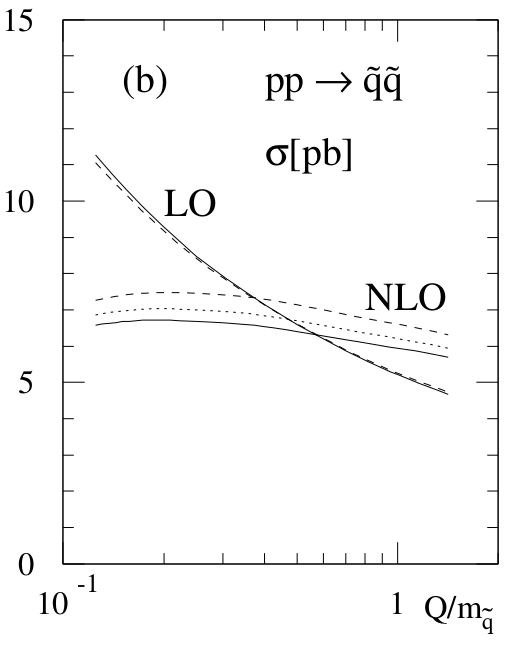
\includegraphics[scale=0.4]{figures_susy_at_hadron_colliders/squark_gluino_LO_NLO.png}
\caption{The dependence on the renormalization/factorization scale $Q$ for the LO and NLO cross sections for squark-squark production at the LHC ($\sqrt{s}=14$ TeV). Parton densities are GRV94 (solid), CTEQ3 (dashed) and MRS(A') (dotted). Mass parameters are $m_{\tilde{q}}=600$ GeV, $m_{\tilde{g}}=500$ GeV and $m_t=175$ GeV. Figure from \cite{beenakker1997squark}.}
\label{Fig:: hadron susy : LO vs NLO beenakker}
\end{figure}


The calculations from \cite{beenakker1997squark} assume degenerate squark masses $m_{\tilde{q}}$, set the 5 lightest quark masses to zero as they are much lighter than the squarks, and the top quark mass to $m_t =175$ GeV. The two free parameters left are then $m_{\tilde{g}}$ and $m_{\tilde{q}}$. This indicates that these might be good features for the learning. The renormalization scheme used is the $\bar{MS}$ scheme. Masses and couplings are renormalized, and the resulting parameters can be found in \cite{beenakker1997squark}.

\subsubsection{Next-to-leading Order Partonic Cross-Section}

As previously discussed, calculations for hadron colliders require first finding the hadronic cross sections. In order to analyze these, scaling functions are introduced \cite{beenakker1997squark} giving the LO+NLO result as
\begin{align}\label{Eq:: susy hadron : Partonic cross section LO+NLO}
\hat{\sigma}_{ij} = \frac{\alpha_s^2(Q^2)}{m^2} \Big\{ &f^B_{ij}(\eta, r) + 4 \pi \alpha_s (Q^2) \Bigg[ f_{ij}^{V+S}(\eta, r, r_t) \nonumber \\ & + f_{ij}^H (\eta, r) + \bar{f}_{ij} (\eta, r) \log \Bigg( \frac{Q^2}{m^2}\Bigg) \Bigg] \Big\},
\end{align}
where $Q^2$ is the renormalization scale, often set to $Q^2 = m^2$, and $m = (\sqrt{p_1^2} + \sqrt{p_2^2})/2$ is the average mass of the produced particles. The scaling functions $f$ are as follows: the Born term $f^B$ from Eq.~(\ref{Eq:: susy hadron : Born term sigma}), the sum of virtual and soft-gluon corrections $f^{V+S}$, the hard gluon corrections $f^H$, and the scale-dependent contributions $\bar{f}$. The partonic cross section depends on the parameters
\begin{align}
&\eta = \frac{s}{4m^2} -1, &r= \frac{m_{\tilde{g}}^2}{m_{\tilde{q}}^2}, &&r_t = \frac{m_t^2}{m^2}.
\end{align}

The energy near the threshold is the base for an important part of the contributions to the cross section \cite{beenakker1997squark}. In this region the scaling functions can be expanded in the low velocity of produced particles $\beta$, leading to the following expressions \cite{beenakker1997squark}
\begin{align}
&f_{qq}^B = \frac{8 \pi \beta m_{\tilde{q}}^2 m_{\tilde{g}}^2}{27(m_{\tilde{q}}^2 + m_{\tilde{g}}^2)^2}, &&f_{q'q}^B = \frac{8 \pi \beta m_{\tilde{q}}^2 m_{\tilde{g}}^2}{9(m_{\tilde{q}}^2 + m_{\tilde{g}}^2)^2} \nonumber \\
& f_{qq}^{V+S} = f_{qq}^B \frac{1}{24 \beta} && f_{q'q}^{V+S} = f_{q'q}^B \frac{1}{24 \beta} \nonumber \\
&f_{qq}^H = f_{qq}^B \Big[\frac{2}{3 \pi^2} \log^2(8 \beta^2) - \frac{7}{2 \pi^2} \log (8 \beta^2) \Big] &&f_{q'q}^H = f_{q'q}^B \Big[\frac{2}{3 \pi^2} \log^2(8 \beta^2) - \frac{19}{6 \pi^2} \log (8 \beta^2) \Big] \nonumber \\
& \bar{f}_{qq} = - f_{qq}^B \frac{2}{3 \pi^2} \log (8 \beta^2) &&\bar{f}_{q'q} = - f_{q'q}^B \frac{2}{3 \pi^2} \log (8 \beta^2).\label{Eq:: susy hadron : Scaling functions near threshold}
\end{align}
The main contributions to the partonic cross section come from this region.

\subsubsection{Hadronic Cross-Section}

As per the above discussion, the partonic cross-sections must be integrated over in order to obtain the total hadronic cross section. A convolution integral over the parton distribution functions yields the expression 
\begin{align}
\sigma(S, Q^2) = \sum_{i,j=q, q, \bar{q}} \int_{\tau}^1dx_1 \int_{\tau/x_1}^1 dx_2 f_i^{h_1} (x_1, Q^2) f_j^{h_2}(x_2, Q^2) \hat{\sigma}_{ij} (x_1x_2S, Q^2)\Big|_{\tau=4m^2/S}.
\end{align}
The integrals are calculated numerically using the VEGAS integration routine \cite{PETERLEPAGE1978192} in \cite{beenakker1997squark}.
The uncertainty due to different parameterizations of the parton densities for the LHC calculations of the NLO terms amount to $\lesssim 13 \%$ at the central scale.

\subsubsection{K-Factor}

To quantify the change in the cross section found by adding NLO terms, the \textit{$K$-factor} is introduced. The $K$-factor is the ratio between the cross sections
\begin{align}
K = \sigma_{NLO}/\sigma_{LO}.
\end{align}
The $K$-factor for squark production for varying mass ratios $m_{\tilde{q}}/m_{\tilde{g}}=2.0$, $ 1.6$, $1.2$, $0.8$ at the LHC is shown in Fig.\ \ref{Fig:: susy hadron : K-factor LHC}. As seen from the figure, the $K$-factor is larger than one and quite stable as a function of the squark mass. 

\begin{figure}
\centering
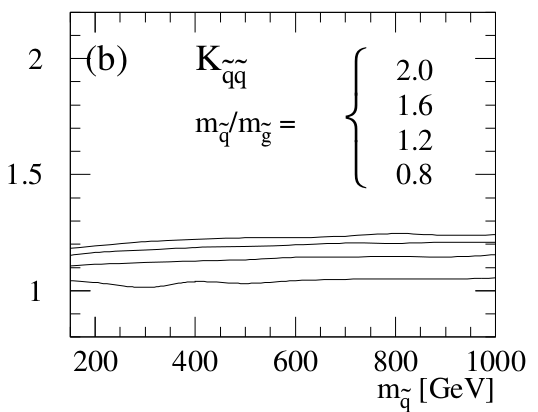
\includegraphics[scale=0.5]{figures_susy_at_hadron_colliders/squark_gluino_K_factor.png}
\caption{The $K$-factors for the LHC ($\sqrt{s}=14$ TeV). Parton densities are GRV94, with scale $Q=m$, and the top squark mass is $m_t=175$ GeV. Figure from \cite{beenakker1997squark}.}
\label{Fig:: susy hadron : K-factor LHC}
\end{figure}


\subsection{State-of-the-art Tools}

There are two numerical tools for the calculation of NLO SUSY cross sections, namely Prospino \cite{beenakker1996prospino} and NLL-fast \cite{beenakker2016nlo+}.

\subsubsection{Prospino}\label{Sec:: susy hadron : Prospino}
\verb|Prospino 2.1| \cite{beenakker1996prospino} is a numerical tool that calculates supersymmetric cross sections to next-to-leading order for non-degenerate squark masses. It uses the $K$-factor to calculate NLO cross sections, by first computing LO cross sections for the 5 or 4 lightest squark flavors. The LO and NLO rates are then calculated for a mean value of the squark mass, and the corresponding $K$-factor is calculated. The LO cross sections for different squarks are then multiplied by the $K$-factor, giving an approximation to the NLO terms for non-degenerate masses. The calculations are outlined in the section above, and are described in more detail in \cite{beenakker1996prospino}. 

\verb|Prospino 2.1| is quite time-consuming, however. Evaluating the strong process cross sections for just a single CMSSM benchmark point takes about 15 minutes of CPU time on a modern processor \cite{balazs2017colliderbit}. 

In addition, as was discovered during the project, \verb|Prospino 2.1| has a weakness in the heavy squark mass space. Consider the cross section for the production of $\tilde{c}_L \tilde{c}_L$. When all squark masses are heavy, but $m_{\tilde{c}_L}$ is slightly lighter than the others, the $K$-factor can be set to zero if the average mass is above threshold ($\tau > s$). This means that $LO \neq 0$ and $NLO =0$, which gives problematic outlier points that cause trouble during learning.



\subsubsection{NLL-fast}

\verb|NLL-fast 2.1| \cite{beenakker1997squark, kulesza2009threshold, kulesza2009soft, beenakker2009soft, beenakker2011squark} computes the hadronic cross sections of gluino and squark pair production including NLO supersymmetric QCD corrections, and the resummation of soft gluon emission at next-to-leading-logarithmic (NLL) accuracy. It also provides an error estimation, based on the errors from renormalization scale dependence and the parton distribution functions. The calculation is done by reading in tables of LO and NLO+NLL results, the scale uncertainty and the PDF and $\alpha_s$ error, and uses fast interpolation to calculate cross sections for any squark and gluino mass within the range $[200, 2500]$ GeV for $\sqrt{s}=8$ TeV. This does mean, however, that \verb|NLL-fast 2.1| is limited in that it only calculates cross sections for mass-degenerate squarks. Since the true total cross section for squark pair production consists of 36 different cross sections for combinations of the 4 lightest quarks, the estimate from \verb|NLL-fast 2.1| is very simplified and unfit for \textit{e.g.} MSSM-24, as shown in a later section.

\subsubsection{Accuracy}

Including the NLO+NLL cross sections has reduced the theoretical error to $10 \%$ for a wide range of processes and masses, see the discussion in \cite{balazs2017colliderbit}. There are other uncertainties, however, such as the ones from the PDFs and $\alpha_s$. These must also be included in the total error estimate. PDFs are based on experimental data, and so the uncertainty increases with the sparticle masses because the PDFs are most poorly constrained at large scales and at large partons $x$.

To illustrate, consider both the gluino and (degenerate) squark mass to be $1.5$ TeV, which is at the edge of what the LHC is able to produce at 8 TeV, as mentioned in the above section. \verb|NLL-fast 2.1| gives errors of $(+24.3 \%, -22.2\%)$ for the PDFs and $(+8.3 \%, -7.3 \%)$ for $\alpha_s$, when using the MSTW2008 NLO PDF
set \cite{Martin:2009iq}. In this case the total error will not be much lower than $25 \%$. However, with new data from the LHC errors from PDFs and $\alpha_s$ will be reduced over time.

Thus, the relative regression errors obtained in this thesis should not exceed $10 \%$, in order to keep the regression errors subdominent.







\chapter{Gaussian Processes}




In this chapter Gaussian process regression is introduced. First, some concepts and terminology in Bayesian statistics are reviewed. The concept of covariance, and how it can be determined by covariance functions is then discussed. The following section introduces the mathematical framework of Gaussian processes, and the Gaussian noise model is used as an example. Bayesian model selection and cross validation are introduced as tools to quantify and improve the quality of predictions.

\section{Introduction to Bayesian Statistics}

There are two general philosophies in statistics, namely \textit{Bayesian} and \textit{frequentist} statistics. To understand where they differ, consider a statement statisticians from both branches would probably state as true
\begin{quote}
\textit{Statisticians use probability to describe uncertainty.}
\end{quote}
The difference between Bayesian and frequentist statistics lies in the definition of the \textit{uncertain}. Since uncertainty is described by probability this understanding must also vary, and one distinguishes between \textit{objective} and \textit{subjective} probability. Consider an example in which a statistician throws a die. Before throwing, he is uncertain about the outcome of the toss. This uncertainty related to the outcome is \textit{objective}: no one can know if he will throw a 1 or a 4. On the other hand, he might also be uncertain about the underlying probability distribution of the toss. Is the die loaded? Is one of the edges sharper than the others? This uncertainty is \textit{subjective}, as it may vary depending on how much information is available about the system, and how that information is used. One of the main critisisms of subjective probability posed by frequentists is that the final probability depends on who you ask.

\subsection{Bayes' Theorem}

To further illustrate the difference between frequentist and Bayesian statistics \textit{Bayes' theorem} \cite{mr1763essay} is introduced. Bayes' theorem can be derived from the familiar rules of probability for random variables $X$ and $Y$ given the information $I$,
\begin{align}\label{Eq:: gaussian process : Sum rule}
P(X | I) + P(\bar{X} | I) = 1,
\end{align}
\begin{align}
 \label{Eq:: gaussian process : Product rule}
P(X, Y | I) = P(X | Y, I)  P(Y | I),
\end{align} 
commonly known as the \textit{sum rule} and \textit{product rule}, respectively. $P(X|I)$ is the probability of outcome $X$ given the information $I$, and $P(X|Y,I)$ is the probability of outcome $X$ given the information $I$ \textit{and} outcome $Y$. The bar over $\bar{X}$ means that the outcome $X$ does \textit{not} happen. The sum rule states that the total probability of the outcomes $X$ and $\bar{X}$ is equal to 1. This is rather intuitive, considering that an event either takes place or not. The product rule concerns the probability of both outcomes $X$ and $Y$. This is equal to the probability of $Y$ times the probability of $X$ given that $Y$ has already ocurred. The product rule can be used to give Bayes' theorem, first formulated by the reverend Thomas Bayes in 1763,
\begin{align}\label{Eq:: gaussian process : Bayes theorem}
P(Y | X, I) = \frac{P(X | Y, I)  P(Y | I)}{P(X | I)}.
\end{align}
Bayes' theorem states that the probability of $Y$ given $X$ is proportional to the probability of $X$ given $Y$, times the probability of $Y$. The proportionality factor is one over the probability of $X$. Surprisingly, there is nothing Bayesian --- in the modern statistical sense ---  about Bayes' theorem. It is merely a reformulation of the rules of logical consistent reasoning by Richard Cox in 1946 \cite{sivia2006data}. Laplace was the one to make Bayes' theorem Bayesian, when he used the theorem to perform inference about probability distributions \cite{laplace1820theorie}. Probability distributions are functions that describe how the probability of a random variable $X$ is distributed, and are denoted $P(X| \Theta, I)$. The \textit{parameters}, $\Theta$, of these functions determine the shape of the distribution, and are \textit{not} random variables. An example of probability distribution parameters are the mean and variance of a Gaussian distribution. Bayes' theorem can be used to find the probability of the \textit{parameters} $\Theta$ given the random variables $X$, and the resulting expression is the \textit{posterior probability distribution}
\begin{align}\label{Eq:: gaussian process : Bayesian inference}
P(\Theta | X , I) = \frac{P(X|\Theta, I) P(\Theta| I)}{P(X | I)},
\end{align}
where $\Theta$ are the probability distribution parameters, $X$ are the random variables, $P(X|\Theta, I)$  and $P(\Theta |I)$ are the \textit{likelihood} and \textit{prior}, respectively, and $P(X|I)$ is a normalization constant called the \textit{marginal likelihood} or evidence. The marginal likelihood is independent of the parameters
\begin{align}
P(X|I) = \int P(X| \Theta, I) P(\Theta | I)~ \text{d} \Theta.
\end{align}
In other words, Eq.~(\ref{Eq:: gaussian process : Bayesian inference}) states the probability of the parameters $\Theta$ given the knowledge of outcomes $X$.

A crucial parting of Bayesian statistics from frequentist statistics is at the introduction of the \textit{prior}, which expresses a probability distribution on the \textit{parameters} of the probability distribution before data. The prior and likelihood are discussed in the next section, while the marginal likelihood is revisited in Sec.~1.4.

\subsection{Priors and Likelihood}\label{Sec:: gaussian process : Priors and Likelihood}

The likelihood $P(X |\Theta, I)$ is simply the probability of the observations $X$ given the parameters of the probability distribution $\Theta$, and is revisited in Sec.~\ref{Sec:: gaussian process : Log Marginal Likelihood}. Conversely, the prior expresses a prior belief or assumption of the parameters, and has to be determined beforehand. As mentioned previously, the measure $P(\Theta | X , I)$ from Eq.~(\ref{Eq:: gaussian process : Bayesian inference}) is called the posterior distribution. This can be thought of as the prior belief, modified by how well this belief fits the data,
\begin{align*}
\text{posterior} = \frac{\text{prior} \times \text{likelihood}}{\text{marginal likelihood}}.
\end{align*}
Consider an example. The statistician from before now sets about tossing a coin. Before tossing he assumes the probability of heads is uniformly distributed, and so adopts a flat, or uniform, prior probability distribution. The uniform distribution is illustrated in the first panel in Fig.~\ref{Fig:: gaussian process : Dice throw }. After one toss he gets heads, and the posterior changes to a function with high probability for heads, and low for tails, illustrated in the second panel. After four tosses, of which two gave heads and two gave tails, the posterior in the third panel shows an equal probabilty for heads and tails, with a wide distribution centered at 0.5. After several tosses the distribution converges to a narrow peak around $0.25$, illustrated in the fourth panel. This indicates an unfair coin that is biased towards tails.

\begin{figure}
\includegraphics[scale=0.76]{figures_gaussian_processes/coin_toss_xd.pdf}
\caption{The posterior probability distribution of the bias-weighting of a coin for the uniform prior, $P(H|I)$. The first panel from the left is before the coin is tossed, the second panel is after 1 toss, the third is after 4 tosses, and the fourth is after 1024 tosses. The posterior converges towards a narrow peak at $0.25$, so the coin is biased.}
\label{Fig:: gaussian process : Dice throw }
\end{figure}


\subsection{Best Estimate and Reliability}\label{Sec:: gaussian process : Best estimate}

Given a posterior distribution $P(X| \mathcal{D}, I)$ over some random variable $X$ where the prior has been modified by some data $\mathcal{D}$, it is important to decide how well the posterior fits the data. As will be shown, the posterior can be approximated by a Gaussian distribution with a mean and variance, where the mean and variance are given by the \textit{best estimate} and the \textit{reliability} of the posterior, respectively. The best estimate $X_0$  is the outcome with the highest probability. In other words, it maximizes the posterior distribution
\begin{align}\label{Eq:: gaussian process : max of posterior}
&\frac{dP}{dX}\Big|_{X_0} = 0, &\frac{d^2P}{dX^2}\Big|_{X_0} < 0,
\end{align}
where $P$ is the posterior $P(X| \mathcal{D}, I)$. The second derivative must be negative to ensure that $X_0$ is, in fact, a maximum. 

Once a best estimate is found, it is important to know how reliable it is. Reliability, or uncertainty, is connected to the width of the distribution. The width of the distribution tells how much the random variables $X$ are smeared out around the mean value $X_0$. A narrow distribution has low uncertainty, while a wide distribution has large uncertainty. As an example, the third panel in Fig.~\ref{Fig:: gaussian process : Dice throw } shows a distribution with a mean value of $0.5$ with large uncertainty, while the fourth panel shows a distribution with mean $0.25$ with small uncertainty. 

The width is found by taking the logarithm \footnote{$L$ is a monotonic function of $P$, so the maximum of $L$ is at the maximum of $P$.} and Taylor expanding the posterior distribution $P(X| \mathcal{D}, I)$
\begin{align}
&L = L(X_0) + \frac{1}{2} \frac{d^2L}{dX^2}\Big|_{X_0} (X-X_0)^2 +... ,&L = \log_e \Big[P(X | \mathcal{D}, I ) \Big]\label{Eq:: gaussian process : Taylor expansion L}
\end{align}
The first term, $L(X_0)$, is just a constant. From Eq.~(\ref{Eq:: gaussian process : max of posterior}) the condition of the best estimate is that $dL/dX|_{X_0} =0$. The dominant term in determining the width is therefore the quadratic term in Eq.~(\ref{Eq:: gaussian process : Taylor expansion L}).

\subsubsection{The Gaussian Distribution}\label{Sec:: gaussian process : The Gaussian Distribution}

Taking the exponential of Eq.~(\ref{Eq:: gaussian process : Taylor expansion L}) and ignoring higher order terms, the posterior can then be approximated as
\begin{align}\label{Eq:: gaussian process : approximate Gaussian}
P(X | \mathcal{D}, I) \approx A \exp \Bigg[ \frac{1}{2} \frac{d^2L}{dX^2}\Big|_{X_0} (X-X_0)^2 \Bigg], 
\end{align} 
where $A = \exp \big[L(X_0) \big]$ is a constant. 

Equation~(\ref{Eq:: gaussian process : approximate Gaussian}) is now in the shape of a \textit{Gaussian distribution}, given by
\begin{align}
P(X| \mu, \sigma^2) = \frac{1}{\sigma \sqrt{2 \pi}} \exp \Bigg[ - \frac{(X- \mu)^2}{2 \sigma^2} \Bigg],
\end{align}
where $\mu$ and $\sigma^2$ are the two parameters of the Gaussian distribution mentioned above. An example of a Gaussian distribution is shown in Fig.~\ref{Fig:: gaussian process : Gaussian distribution}. The parameter $\mu$ is the \textit{mean value} of $X$, which will be written as $ m(X)$, and $\sigma^2$ is shorthand for the \textit{variance} of the distribution around the mean $m(X)$, which will be written as $\mathbb{V}(X)$. The variance is discussed further below. The mean and variance for the approximated Gaussian distribution of $P(X|\mathcal{D}, I)$ are then given by
\begin{align}
m(X) = X_0\text{, }~ \mathbb{V}(X) = \Big( - \frac{d^2L}{dX^2} \Big)^{-1/2}.
\end{align}

The Gaussian distribution is also referred to as the \textit{normal distribution}, and a Gaussian distribution with mean $m(X)= \mu$ and variance $\mathbb{V}(X)=\sigma^2$ is therefore written as $\mathcal{N}(\mu, \sigma^2)$. The notation $X \sim \mathcal{N}(\mu, \sigma^2)$ means a \textit{random variable $X$ drawn from a Gaussian distribution with mean $\mu$ and variance $\sigma^2$}. The Gaussian distribution is symmetric with respect to the maximum at the mean $\mu$, and has a full width at half maximum (FWHM) at around $2.35 \sigma$, where $\sigma = \sqrt{\sigma^2}$ is the standard deviation.  

In Gaussian process regression of a function, $f(\textbf{x}), ~\textbf{x} \in \mathbb{R}^D$, the Gaussian distribution is central, as the basic idea is to predict a Gaussian distribution over function values $f(\textbf{x})$ for each input vector $\textbf{x}$. Gaussian processes are discussed in Sec.~\ref{Sec: gaussian process : Gaussian Process Regression}, so for now it will suffice to sum up that the quality of a posterior distribution, $P(X| \mathcal{D}, I)$, can be summed up in two measures: the best estimate and the reliability. These can be seen as the mean and variance of a Gaussian distribution $\mathcal{N}(m(X), \mathbb{V}(X))$, where
\begin{align}
m(X)~&:~ \text{Mean of }X,\\
\mathbb{V}(X)~&:~ \text{Variance of }X.
\end{align}


\subsubsection{Variance}

Now that some basics of Gaussian processes have been covered, a more formal definition of the variance of a distribution is in order. The variance $\mathbb{V} (X)$ is defined as the expectation value of the square of deviations from the mean. The expectation value of a random variable $X$ with a probability distribution $P(X | I)$ is here written as $\mathbb{E}[X]$, and defined as
\begin{align}
\mathbb{E}[X] = \int X P(X | I) ~\text{d}X ~:~ \text{Expectation value of }X.
\end{align}
 For the posterior probability distribution $P(X| \mathcal{D}, I)$ the variance of the random variable $X$ is then given by \cite{sivia2006data}
\begin{align}\label{Eq:: gaussian process : variance X 1dim}
\mathbb{V}(X) = \mathbb{E} \big[ (X - X_0)^2 \big] = \int \int (X - X_0)^2 P (X| \mathcal{D}, I) ~\text{d}X.
\end{align}
The variance in $X$ is often denoted $\sigma_X^2 = \mathbb{V}(X)$, and its square root is the \textit{standard deviation} $\sqrt{\sigma^2_X} = \sigma_X$. 



\begin{figure}
\centering
\includegraphics[scale=1.0]{figures_gaussian_processes/gaussian_distribution_xd.pdf}
\caption{A Gaussian probability distribution. The maximum is at the mean value $\mu$, with a full width at half maximum (FWHM) at around $2.35 \sigma$. Figure from \cite{sivia2006data}.}
\label{Fig:: gaussian process : Gaussian distribution}
\end{figure}

\subsection{Covariance}\label{Sec:: gaussian process : Covariance}

In distributions over several random variables, $P(X_i| \mathcal{D}, I)$, varying one variable can affect the variance of another variable. This is called \textit{covariance}. For these distributions the equations are not as simple to solve as in Eq.\ (\ref{Eq:: gaussian process : Taylor expansion L}). In the case of several random variables $X_i$, a set of \textit{simultaneous equations} must be solved to get the best estimate
\begin{align}\label{Eq:: gaussian process : Best estimate X_i}
&\frac{dP}{dX_i} \Big|_{X_{0j}} =0, &&\frac{d^2P}{dX_i^2} \Big|_{X_{0j}} < 0
\end{align}
To simplify expressions consider the problem in two dimensions, so that $\{ X_i \} = (X, Y)$. Analogously to Eq.~(\ref{Eq:: gaussian process : Taylor expansion L}), the Taylor expansion of $L = \log_e \Big[ P(X, Y |I) \Big]$ is found
\begin{align}\label{Eq:: gaussian process : Taylor expansion L_i}
L =& L(X_0, Y_0) + \frac{1}{2} \Big[ \frac{d^2L}{dX^2}  \Big|_{X_0, Y_0}(X-X_0)^2 \nonumber \\
& + \frac{d^2L}{dY^2}  \Big|_{X_0, Y_0}(Y-Y_0)^2 + 2 \frac{d^2L}{dXdY}  \Big|_{X_0, Y_0}(X-X_0)(Y-Y_0) \Big] +...
\end{align}
There are now four partial derivatives, reduced to three using the rules for mixed partial derivatives $\frac{\partial^2}{\partial X \partial Y} = \frac{\partial^2}{\partial Y \partial X}$. Writing the quadratic terms of Eq.~(\ref{Eq:: gaussian process : Taylor expansion L_i}) in matrix form gives
\begin{align}
Q = 
\begin{pmatrix}
X-X_0 & Y -Y_0
\end{pmatrix}
\begin{pmatrix}
A & C\\
C & B
\end{pmatrix}
\begin{pmatrix}
X -X_0\\
Y-Y_0
\end{pmatrix},
\end{align}
where the matrix elements are
\begin{align}\label{Eq:: gaussian process : covariance matrix ABC}
&A = \frac{\partial^2 L}{\partial X^2} \Big|_{X_0, Y_0}, &B = \frac{\partial^2 L}{\partial Y^2} \Big|_{X_0, Y_0}, &&C = \frac{\partial^2 L}{\partial X \partial Y} \Big|_{X_0, Y_0}.
\end{align}

The expression for the variance of $X$ for the distribution $P(X,Y| I)$ is very similar to Eq.~(\ref{Eq:: gaussian process : variance X 1dim}), except for an additional integral over the random variable $Y$
\begin{align}
\mathbb{V}(X) = \sigma^2_X = \mathbb{E} \big[ (X-X_0)^2 \big] = \int \int (X-X_0)^2 P(X,Y | \mathcal{D}, I) ~\text{d}X\text{d}Y.
\end{align}
A similar expression, $\sigma_Y^2$, can be found for $Y$ by substituting $X$ and $Y$. 

The simultaneous deviations of the random variables $X$ and $Y$ is the aforementioned covariance, often written as $\sigma_{XY}^2$. In two dimensions the covariance is given by
\begin{align}
\sigma_{XY}^2 = \mathbb{E} \big[(X - X_0) (Y - Y_0) \big] =\int \int (X - X_0) (Y - Y_0) P (X, Y | \mathcal{D}, I) ~\text{d}X\text{d}Y.
\end{align}
The covariance indicates how an over- or underestimation of one random variable affects another. If, for example, an overestimation of $X$ leads to an overestimation of $Y$, the covariance is positive. An example of positive covariance is shown in the third panel of Fig.~\ref{Fig:: gaussian process : Covariance illustrated}. If the overestimation of $X$ has little or no effect on the estimation of $Y$, the covariance is negligible or zero $|\sigma_{XY}| \ll \sqrt{\sigma_X^2 \sigma_Y^2}$, as seen in the first panel of Fig.~\ref{Fig:: gaussian process : Covariance illustrated}. The second panel shows negaitve covariance.

\subsubsection{Covariance Matrix}

The variances and covariances are the elements of the \textit{covariance matrix}. For $N$ random variables $X_1, ...,X_N$ the covariance matrix is an $N \times N$-matrix. The covariance matrix for $X$ and $Y$ is here denoted $\text{cov}(X,Y)$, and it can be shown that \cite{sivia2006data}
\begin{align}
\text{cov}(X,Y) = 
\begin{pmatrix}
\sigma_X^2 & \sigma_{XY}^2\\
\sigma_{XY}^2 & \sigma_Y^2
\end{pmatrix}
= - \begin{pmatrix}
A & C\\
C & B
\end{pmatrix}^{-1},
\end{align}
where $A$, $B$ and $C$ are the covariances defined in Eq.~(\ref{Eq:: gaussian process : covariance matrix ABC}).

To sum up, the posterior probability distribution over a random variable $X$ is denoted $P(X | \mathcal{D}, I)$ which can be approximated as a Gaussian distribution $\mathcal{N}(m(X), \mathbb{V}(X))$, where the mean is the best estimate of $P(X | \mathcal{D}, I)$ and the variance is the associated reliability. The Gaussian distribution is defined by the mean value $m(X)$ and the variance $\mathbb{V}(X)$. For distributions over several random variables $X_i$ one can also find the covariance $\sigma_{X_i X_j}^2$, and all variances and covariances are contained in the covariance matrix $\text{cov}(X_i)$. In the next section \textit{covariance functions} are introduced, which are used to calculate the elements of the covariance matrix.

\begin{figure}
\centering
\includegraphics[scale=1.0]{figures_gaussian_processes/covariance_xd.pdf}
\caption{A schematic illustration of covariance and correlation. (a) The contours of a posterior pdf with zero covariance, where the inferred values of $X$ and $Y$ are uncorrelated. (b) The corresponding plot when the covariance is large and negative; (c) The case of positive correlation.}
\label{Fig:: gaussian process : Covariance illustrated}
\end{figure}


\section{Covariance Functions}\label{Sec:: gaussian processes : Covariance functions}


As mentioned in Sec.~\ref{Sec:: gaussian process : Covariance}, the elements of a covariance matrix can be determined by \textit{covariance functions}, or \textit{kernels}. A function that maps two arguments $\textbf{x},\textbf{x}' \in \mathcal{X}$ into $\mathbb{R}$, where $\mathcal{X}$ is the input space, is generally called a kernel $k$. Covariance functions are symmetric kernels, meaning that $k(\textbf{x}, \textbf{x}') = k(\textbf{x}', \textbf{x})$. In this project both kernel and covariance function are taken to mean covariance function. 

In Gaussian processes, which are discussed in Sec.~\ref{Sec:: gaussian process : Gaussian Processes}., the covariance between two function values $f(\textbf{x})$ and $f(\textbf{x}')$, where $\textbf{x}$ and $\textbf{x}'$ are input vectors, is given by the covariance of the input vectors. Further, the covariance of the input vectors is given by a kernel, 
\begin{align}
\text{cov}(f(\textbf{x}), f(\textbf{x}')) = k(\textbf{x}, \textbf{x}').
\end{align}
The matrix containing all the covariance elements is, as mentioned, called the \textit{covariance matrix}, or the \textit{Gram matrix} $K$, whose elements are given by
\begin{align}\label{Eq:: covariance matrix}
K_{ij} = k(\textbf{x}_i, \textbf{x}_j).
\end{align}
Note that a covariance matrix calculated using a covariance function $k$ is denoted by a capital $K$.

A kernel function that only depends on the difference between two points, $\textbf{x}-\textbf{x}'$, is called \textit{stationary}. This means that the function is invariant to translations in input space. If, in addition, it only depends on the length $r=|\textbf{x}-\textbf{x}'|$, the function is \textit{isotropic}\footnote{Invariant to rigid rotations in input space.}.  Isotropic functions are commonly referred to as \textit{radial basis functions} (RBFs), as they are only functions of $r$. 

The covariance function can also depend on the dot product, $\textbf{x} \cdot \textbf{x}'$, and is then called a \textit{dot product} covariance function. The most important covariance functions for this project are the squared exponential covariance function and the Mat\'{e}rn class of covariance functions.




\subsection{The Squared Exponential Covariance Function}

The \textit{squared exponential covariance function} (SE) has the form 
\begin{align}\label{Eq:: gaussian process : Squared Exponential Kernel}
k_{\mathrm{SE}} (r) = \exp \Big( - \frac{r^2}{2 \ell^2} \Big),
\end{align} 
where $\ell$ is the \textit{characteristic length scale}. Equation~(\ref{Eq:: gaussian process : Squared Exponential Kernel}) is sometimes also called the \textit{radial basis function} (RBF). The length scale, $\ell$, determines the smoothness of the function. It can be loosely interpreted as how far you need to move (along a particular axis) in input space for the function values to become uncorrelated. For a large length scale one should expect a very slowly varying function, while a shorter length scale means a more rapidly varying function, see the illustration in Fig.~\ref{Fig:: gaussian process : ell variation example}. The SE is infinitely differentiable and therefore very smooth. Stein \cite{steininterpolation} argues that such strong smoothness assumptions are unrealistic for most physical problems, and recommends another class of kernels, namely the \textit{Mat\'{e}rn class of covariance functions}.

\begin{figure}
\centering
\includegraphics[scale=1.5]{figures_gaussian_processes/length_scales_xd.pdf}
\caption{The effect of varying the length scale $\ell$. A long length scale (blue) gives a smooth, slowly varying function, while a short length scale (red) gives a more staccato, quickly varying function.}
\label{Fig:: gaussian process : ell variation example}
\end{figure}

%The SE is implemented in \verb|scikit-learn| under the name radial basis function (RBF), and may be called in the following way for length scale $10$, with bounds on the length scale $[0.01, 100]$
%\begin{lstlisting}
%from sklearn.gaussian_process.kernels import RBF
%rbf = RBF(length_scale=10, length_scale_bounds=(1e-2, 1e2))
%\end{lstlisting}

\subsection{The Mat\'{e}rn Class of Covariance Functions}\label{Sec:: gaussian process : Matern Class of Covariance Functions}

The \textit{Mat\'{e}rn class of covariance functions} is given by
\begin{align}\label{Eq:: gaussian process : Matern class of covariance functions}
k_{\mathrm{Mat\acute{e}rn}} (r) = \frac{2^{1- \nu}}{\Gamma (\nu)} \Big( \frac{\sqrt{2 \nu} r	}{\ell} \Big)^{\nu} K_{\nu} \Big( \frac{\sqrt{2 \nu}r}{\ell} \Big),
\end{align}
where $\nu, \ell > 0$, and $K_{\nu}$ is a modified Bessel function \cite{abramowitz1964handbook}. The hyperparameter $\nu$ controls the smoothness of the function. For $\nu \rightarrow \infty$ this becomes the SE kernel, and for $\nu = 1/2$ is becomes the very rough absolute exponential kernel $k(r) = \exp (-r/\ell)$. In the case of half integer $\nu$, $\nu = p + \frac{1}{2}$ for $p \in \mathbb{N}$, the covariance function is simply the product of an exponential and a polynomial
\begin{align}
k_{\nu=p+\frac{1}{2}} = \exp \Big(- \frac{\sqrt{2 \nu} r	}{\ell} \Big) \frac{\Gamma(p+1)}{\Gamma(2p + 1)} \sum^p_{i=0} \frac{(p+i)!}{i!(p-i)!} \Big( \frac{\sqrt{8 \nu} r	}{\ell} \Big)^{p-i}.
\end{align}
In machine learning the two most common cases are for $\nu = 3/2$ and $\nu = 5/2$
\begin{align}
k_{\nu = 3/2}(r) &=  \Big(1 + \frac{\sqrt{3}r}{\ell} \Big) \exp \Big( -\frac{\sqrt{3}r}{\ell} \Big),\\
k_{\nu = 5/2}(r) &=  \Big(1 + \frac{\sqrt{5}r}{\ell}  + \frac{5r^2}{3 \ell^2}\Big) \exp \Big( -\frac{\sqrt{5}r}{\ell} \Big).
\end{align}

%In \verb|scikit-learn| the hyperparameter $\nu$ is fixed, and so not optimized during training. The Mat\'{e}rn kernel is considered more appropriate for physical processes \cite{rasmussen2006gaussian}, and may be called in \verb|scikit-learn| in the following way for length scale 10, length scale bounds $[0.01, 100]$ and $\nu = 3/2$
%\begin{lstlisting}
%from sklearn.gaussian_process.kernels import Matern
%matern = Matern(length_scale=10, length_scale_bounds=(1e-2, 1e2), nu=1.5)
%\end{lstlisting}


\subsection{Noise}\label{Sec:: gaussian process : Noise Covariance Function}


The covariance function can also contain information about noise in the data. In the case where the noise, $\varepsilon$, follows a Gaussian distribution $\varepsilon \sim \mathcal{N}(0, \sigma_n^2)$, the noise is represented by adding the variance, $\sigma_n^2$, to the diagonal of the covariance matrix
\begin{align}
k(\textbf{x}_i, \textbf{x}_j)_{noise} = \sigma^2_n \delta_{ij},
\end{align}
where $\delta_{ij}$ is the Kronecker-delta. The model where the noise is assumed to follow a Gaussian distribution is called the \textit{Gaussian noise model}, and is discussed in Sec.~\ref{Sec: gaussian process : Gaussian Noise Model}. %In \verb|scikit-learn| this can be implemented either by giving a fixed noise level \verb|alpha| to the regressor function, or by using the \verb|WhiteKernel|, which estimates the noise level from the data. %This kernel is implemented in \verb|scikit-learn| in the following way for noise level $0.001$ with bounds $[10^{-10}, 1]$
%\begin{lstlisting}
%from sklearn.gaussian_processes.kernels import %WhiteKernel
%whitenoise = WhiteKernel(noise_level=0.001, noise_level_bounds=(1e-10,1))
%\end{lstlisting}

\subsection{Hyperparameters}\label{Sec:: gaussian process : Hyperparameters}

The SE kernel in Eq.~(\ref{Eq:: gaussian process : Squared Exponential Kernel}) and the Mat\'{e}rn kernel in Eq.~(\ref{Eq:: gaussian process : Matern class of covariance functions}) are both isotropic, \textit{i.e.} functions only of the distance between input points, $r$. Isotropic kernels can, however, be generalized to an anisotropic form by setting
\begin{align}
r^2(\textbf{x}, \textbf{x}') = (\textbf{x} - \textbf{x}')^T M(\textbf{x} - \textbf{x}'),
\end{align}
where $M$ is some positive definite matrix. The matrix $M$ can take multiple forms, such as 
\begin{align}
&M_1 = \ell^{-2} \mathbb{I} , &M_2 = \text{diag}(\vec{\ell})^{-2},
\end{align}
where $\ell^2$ is a scalar, and $\vec{\ell}$ is a vector of the same dimension as the input vectors $\textbf{x}$, $\textbf{x}'$. Choosing $\vec{\ell}$ to be a vector in stead of a scalar is in many cases useful, especially if the input vector $\textbf{x}$ contains values of different scales.

The matrix $M$ is now part of the \textit{hyperparameters} of the kernel. Each kernel has a vector of hyperparameters, denoted $\vec{\theta}$. An example is the following generalisation of the SE kernel, 
\begin{align}
k(\textbf{x}_i, \textbf{x}_j) = \sigma_f^2 \exp \big(- \frac{1}{2} (\textbf{x}_i - \textbf{x}_j)^T M (\textbf{x}_i - \textbf{x}_j) \big) + \sigma_n^2 \delta_{ij},
\end{align}
where $\sigma_f$ is a scaling factor and $\sigma_n^2$ is the Gaussian noise parameter, discussed in Sec.~\ref{Sec:: gaussian process : Noise Covariance Function}. The hyperparameters of this kernel are $\vec{\theta} = (\{M\}, \sigma^2_f, \sigma_n^2)^T$, where $\{M\}$ denotes the parameters in the symmetric matrix $M$. 
%The length scale can be set to a vector in \verb|scikit-learn| by giving the \verb|length_scale| parameter as a \verb|numpy| array of the same dimension as the input vector $\textbf{x}$.

\subsubsection{Other Covariance Functions}

There are several other types of covariance functions that are not discussed here. In addition, kernels can be multiplied and summed to form new kernels, making the space of possible kernels infinite. For further details see Chapter 4 in \cite{rasmussen2006gaussian}.




\section{Gaussian Process Regression}\label{Sec: gaussian process : Gaussian Process Regression}

Gaussian processes (GP) is a supervised machine learning method, designed to solve regression and probabilistic classification problems. Only regression is considered here. This section begins by introducing Gaussian processes and important notation, first in a general sense, and then in the function space view. Then distributions over functions are considered, followed by a short discussion on how functions can be drawn from these distributions. Finally, a quick overview of the noise-free model and the Gaussian noise nodel, and their covariance matrices, are given.

\subsubsection{Gaussian Processes}\label{Sec:: gaussian process : Gaussian Processes}

Consider a set of points $\mathcal{D} = \{\textbf{x}_i, y_i\}$, where $y$ is some (possibly noisy) function of $\textbf{x}$, $y(\textbf{x}) = f(\textbf{x}) + \varepsilon$. Here, $\varepsilon$ is the noise and $f(\textbf{x})$ is the true value of the function. These points are illustrated by the black dots in Fig.~\ref{Fig:: gaussian process : GP illustration}. In machine learning $\mathcal{D}$ is the \textit{training data}, as it is used to train the model. It consists of \textit{features}, which are the components of the input vectors $\textbf{x}_i$, and \textit{targets}, which are the function values $y_i$. The set of points is discrete, so there is some $\textbf{x}^*$ for which the target $y^*$ is unknown. The test point $\textbf{x}^*$ is marked on the $x$-axis in Fig.~\ref{Fig:: gaussian process : GP illustration}.

Gaussian processes (GP) predict a Gaussian distribution \textit{over function values} at this point $\textbf{x}^*$. The distribution for a single test point $\textbf{x}^*$ has a corresponding mean $m(\textbf{x}^*)$ and variance $\mathbb{V}(\textbf{x}^*)$. Note that the mean $m(\textbf{x}^*)$ \textit{is not the mean of the input vector} $\textbf{x}^*$, but rather \textit{the mean of function values} $f(\textbf{x})$ \textit{evaluated at} $\textbf{x}^*$. The GP prediction for the target value $y^*=f(\textbf{x}^*)$ is the mean $m(\textbf{x}^*)$. Similarly, the variance, $\mathbb{V}(\textbf{x}^*)$, is in fact the variance in function values $f(\textbf{x}^*)$, or the width of the Gaussian distribution (red line) in the $y$-direction in Fig.~\ref{Fig:: gaussian process : GP illustration}. The mean value $y^*$ is drawn as a blue cross in Fig.~\ref{Fig:: gaussian process : GP illustration}. As will be shown, the predicted target $y^*$ is a linear combination of the known targets $y_i$, where the weights are controlled by the covariances between training points $\textbf{x}_i$ and the test point $\textbf{x}^*$.  


\begin{figure}
\centering
\includegraphics[scale=1.5]{figures_gaussian_processes/gp_illustration_xd.pdf}
\caption{An illustration of a GP prediction of the target value $y^*$ (blue cross), given the known set of points $\{x_i, y_i\}$ (black dots). The prediction is a Gaussian distribution in $y$ with mean $y^*$ and variance $\sigma^2$. The Gaussian distribution is drawn in red with $y$ on the vertical axis, with uncertainty in the $y$-direction.}
\label{Fig:: gaussian process : GP illustration}
\end{figure}

\subsubsection{Some Notation}

As Gaussian process regression is notoriously confusing, it is helpful to begin with some notation. 

As discussed in Sec.~\ref{Sec: gaussian process : Gaussian Process Regression}, the Gaussian distribution with a mean $\mu$ and variance $\sigma^2$ is denoted $\mathcal{N}(\mu, \sigma^2)$. The distribution can be over a single random variable, \textit{e.g.} $f$, or a finite set of random variables, $f_i$. A Gaussian distribution over several random variables is called a \textit{multivariate Gaussian distribution}. The $n$ random variables $f_i, ~i=1,...,n$ drawn from a multivariate Gaussian distribution make up the $n$-dimensional vector $\textbf{f}$. The mean values, $\mu_i$, are then contained in the $n$-dimensional \textit{mean vector} $m(\textbf{f})$. The variance, $\sigma^2$, is replaced by an $n \times n$-dimensional covariance matrix, $\text{cov}(\textbf{f}, \textbf{f})$. The multivariate Gaussian distribution over $\textbf{f}$ is written as
\begin{align}
\textbf{f} \sim \mathcal{N} \big(m(\textbf{f}), ~\text{cov}(\textbf{f},\textbf{f})  \big).
\end{align}  

For $n$ points $\{\textbf{x}_i , y_i\}$, where $\textbf{x}_i$ is an $m$-dimensional feature vector and $y_i$ is the target, the features comprise the $n \times m$-matrix $X$. The targets make up the corresponding $n$-dimensional vector $\textbf{y}$. A central assumption in Gaussian processes is that the covariance between targets $y_i$, $y_j$ is given by the covariance of their features $\textbf{x}_i$, $\textbf{x}_j$
\begin{align}
\text{cov}(y_i, y_j) = k(\textbf{x}_i, \textbf{x}_j),
\end{align}
where $k(\textbf{x}_i, \textbf{x}_j)$ is a covariance function, as described in Sec.~\ref{Sec:: gaussian processes : Covariance functions}. In Gaussian processes the distribution over target values $\textbf{f}$ with feature matrix $X$ will therefore be written
\begin{align}\label{Eq:: gaussian process : Normal distribution GP}
\textbf{f} \sim \mathcal{N} \big(~m( \textbf{f} ), K(X, X) ~\big),
\end{align}
where $K(X,X)$ is the covariance matrix containing the covariances of the features contained in $X$, calculated using the covariance function $k(\textbf{x}, \textbf{x}')$.

Finally, a Gaussian process will be denoted $\mathcal{GP}$. It may be difficult to distinguish between a Gaussian \textit{distribution}, $\mathcal{N}$, and a Gaussian \textit{process}, $\mathcal{GP}$. The difference can be thought of as the difference between a finite collection of function values $f_i = f(\textbf{x}_i)$, and the continuous function, $f(\textbf{x})$. The former can be viewed as a vector $\textbf{f}$, and can be drawn from a distribution such as the one in Eq.~(\ref{Eq:: gaussian process : Normal distribution GP}), $\textbf{f} \sim \mathcal{N}(m(\textbf{f} ), K(X, X))$. The latter is a \textit{function}, drawn from a distribution \textit{over functions}, where the mean $m(\textbf{x})$ and covariances $k(\textbf{x}, \textbf{x}')$ are functions as well. A function $f(\textbf{x})$ drawn from a Gaussian process is written as 
\begin{align}
f(\textbf{x}) \sim \mathcal{GP} (m(\textbf{x}), k(\textbf{x}, \textbf{x}')).
\end{align}

\subsubsection{Function Space View}

Gaussian processes provide distributions over functions $\mathcal{GP}$. It is therefore useful to consider the problem in the function space view introduced in \cite{rasmussen2006gaussian}. For a function $f(\textbf{x})$ the Gaussian process \textit{mean function}, $m(\textbf{x})$, and \textit{covariance function}, $k(\textbf{x}, \textbf{x}')$, are defined as
\begin{align}
m(\textbf{x}) &= \mathbb{E}[f(\textbf{x})],\\
k(\textbf{x}, \textbf{x}') &= \mathbb{E} [(f(\textbf{x}) - m(\textbf{x}))(f(\textbf{x}') - m(\textbf{x}'))].
\end{align}
In other words, the mean $m(\textbf{x})$ is the expected value of the function $f(\textbf{x})$ at $\textbf{x}$, and the covariance function is the expected value of the simultaneous deviations of $f(\textbf{x})$ from the mean $m(\textbf{x})$ at $\textbf{x}$, and $f(\textbf{x}')$ from the mean $m(\textbf{x}')$ at $\textbf{x}'$. As mentioned, the mean and covariance are now \textit{functions} of the input vector $\textbf{x}$. This means that for every input vector $\textbf{x}$, there is a Gaussian distribution over function values with a mean $m(\textbf{x})$ and covariance given by $k(\textbf{x}, \textbf{x}')$. This is a generalization of the single test point in Fig.~\ref{Fig:: gaussian process : GP illustration}, where every point $\textbf{x}^*$ gets a similar distribution.

The collection of Gaussian distributions over functions that are now a function of the input vector $\textbf{x}$ are the Gaussian processes, $\mathcal{GP}$. In the same way that a random variable is drawn from a distribution, random functions can be drawn from the $\mathcal{GP}$,
\begin{align}
f(\textbf{x}) \sim \mathcal{GP}(m(\textbf{x}), k(\textbf{x}, \textbf{x}')).
\end{align}
How functions are drawn from distributions is discussed in more detail in a later section.

The covariance between two points $f(\textbf{x})$ and $f(\textbf{x}')$ is determined by the covariance function $k(\textbf{x}, \textbf{x}')$, as discussed in Sec.~\ref{Sec:: gaussian processes : Covariance functions}. The distribution $\mathcal{GP}$ is over function values, and so the covariance function calculates the covariance between the \textit{function values}, $f(\textbf{x}_i)$ and $f(\textbf{x}_j)$, and \textit{not} the input vectors, $\textbf{x}_i$ and $\textbf{x}_j$. Rather, the covariance between two function values is a function of the input vectors. Consider again the illustration in Fig.~\ref{Fig:: gaussian process : ell variation example}. The variation in function values $f(\textbf{x}_i)$ and $f(\textbf{x}_j)$ depends on the distance between the points $\textbf{x}_i$ and $\textbf{x}_j$, and the characteristic length scale of the process. If the length scale is large, the two input vectors $\textbf{x}_i$ and $\textbf{x}_j$ can be far away, and still have similar function values $f(\textbf{x}_i)$ and $f(\textbf{x}_j)$. For short length scales, however, nearby points can have very different function values, because the function varies rapidly.

\subsubsection{Distributions over Functions}

Functions can be drawn from the Gaussian process, $\mathcal{GP}(m(\textbf{x}), k(\textbf{x}, \textbf{x}'))$, with mean $m(\textbf{x})$ and covariance $k(\textbf{x}, \textbf{x}')$, as mentioned above. All functions $f(\textbf{x})$ that are drawn from this distribution must have a covariance between function values $f(\textbf{x})$, $f(\textbf{x}')$ determined by the covariance function $k(\textbf{x}, \textbf{x}')$. If for example the covariance function has a large length scale, quickly varying functions are not allowed. The mean of the distribution, $m(\textbf{x})$, is \textit{not} the mean value of each function $f(\textbf{x})$ drawn from $\mathcal{GP}$, but rather the mean function value you would get in $\textbf{x}$ if you drew enough functions from $\mathcal{GP}$. Drawing functions from a distribution in this way will be referred to as \textit{drawing samples}.

Gaussian processes are Bayesian in that there is a prior and a posterior distribution over functions, where the posterior is obtained by conditioning the prior on the training data. Consider the $n^* \times m$-matrix of test points $X^*$, containing $n^*$ test points $\textbf{x}_i^*$, with unknown function values $f(\textbf{x}^*)$. Using the kernel on the matrix $X^*$ gives the covariance matrix, as discussed in Sec.~\ref{Sec:: gaussian processes : Covariance functions}. The covariance matrix $K(X^*, X^*)$ now contains the covariance of all test points $\textbf{x}^*_i$, calculated using the covariance function $k(\textbf{x}_i^*, \textbf{x}_j^*)$. Combined with an initial mean of zero \footnote{The mean does not have to be zero, it could for example be the mean of the training data.} one obtains the \textit{prior} distribution of predicted target values $\textbf{f}^*$
\begin{align}
\textbf{f}^* \sim \mathcal{N} (\vec{0}, K(X^*, X^*)).\label{Eq:: gaussian process : Prior GP}
\end{align} 
This distribution contains the prior assumptions about the function values $f(\textbf{x})$, in that the smoothness of the function and the correlation between function values are encoded in the covariance matrix. This is the prior probability distribution discussed in Sec.~\ref{Sec:: gaussian process : Priors and Likelihood}, that will be modified by the data to provide the posterior probability distribution. The choice of kernel is therefore one of the most important steps in learning with GPs. 

\subsubsection{Noise-Free Model}

Now consider the addition of training data to the prior distribution in Eq.~\ref{Eq:: gaussian process : Prior GP}, in the form of a noise-free set of $n$ training points $\{\textbf{x}_i, y_i\}$, so that $y = f(\textbf{x})$. The input vectors $\textbf{x}_i$ form the $n \times m$-matrix $X$, where the rows are the input vectors. The training targets $y_i$ form the corresponding $n$-dimensional vector $\textbf{f}$. The test points are still contained in the $n^* \times m$ matrix $X^*$. The goal is to predict an $n^*$-dimensional vector $\textbf{f}^*$ containing the predictions of the function values at the points $\textbf{x}^*_i$, which is conditioned on the known function values $\textbf{f}$. 

The joint distribution of training outputs, $\textbf{f}$, and test outputs, $\textbf{f}^*$, according to the prior in Eq.~\ref{Eq:: gaussian process : Prior GP} is
\begin{align}
\begin{bmatrix}
\textbf{f}\\
\textbf{f}^*
\end{bmatrix}
\sim 
\mathcal{N} \Bigg(
\boldsymbol{0},
\begin{bmatrix}
K(X, X) & K(X, X^*)\\
K(X, X^*) & K(X^*, X^*)
\end{bmatrix}
 \Bigg),
\end{align}
where, as before, $K(X_i, X'_j)$ is the covariance matrix between the sets of points $\{ \textbf{x}_i \}$ and $\{\textbf{x}'_j \}$ calculated using the covariance function $k(\textbf{x}_i, \textbf{x}'_j)$. By conditioning the distribution of $\textbf{f}^*$ on the observations $\textbf{f}$,  the posterior distribution over $\textbf{f}^*$ is obtained\footnote{For more details, see Appendix A.2 in \cite{rasmussen2006gaussian}.}  \cite{rasmussen2006gaussian} 
\begin{align}\label{Eq:: gaussian process : Posterior GP noise-free}
\textbf{f}^* \big| X^*, X, \textbf{f} \sim \mathcal{N}&(K(X^*, X)K(X, X)^{-1} \textbf{f},\\ &K(X^*, X^*) - K(X^*, X)K(X, X)^{-1}K(X, X^*)),
\end{align}
where $\textbf{f}^* | X^*, X, \textbf{f}$ means the target values $\textbf{f}^*$ for the features $X^*$, given the known features $X$ and targets $\textbf{f}$. The prior in Eq.~\ref{Eq:: gaussian process : Prior GP} has now been modified by the data $X$, $\textbf{f}$ to give the posterior in Eq.~\ref{Eq:: gaussian process : Posterior GP noise-free}, leaving two distributions from which function values can be drawn.


\subsubsection{Drawing Samples}

To generate samples $\textbf{f} \sim \mathcal{N}(\textbf{m}, K)$ with mean $\textbf{m}$ and covariance matrix $K$ using a scalar Gaussian generator\footnote{A scalar Gaussian generator generates random numbers from a Gaussian distributions, and can be found in most programming enviroments, such as the \verb|random| environment in \verb|Python|.}, one proceeds as follows: first the Cholesky decomposition --- also known as the matrix square root ---  $L$ of the covariance matrix is found using $K = LL^T$. $L$ is a lower triangular matrix. A vector $\textbf{u}$ is then generated by multiple calls to the scalar Gaussian generator $\textbf{u} \sim \mathcal{N}(0, I)$. Then $\textbf{f} = \textbf{m} + L \textbf{u}$ has the desired distribution with mean $\textbf{m}$ and covariance $L \mathbb{E} [\textbf{u} \textbf{u}^T]L^T = LL^T = K$, as described in \cite{rasmussen2006gaussian}.

Using the method described above, random functions have been drawn from the prior and posterior in Eq.~\ref{Eq:: gaussian process : Prior GP} and Eq.~\ref{Eq:: gaussian process : Posterior GP noise-free}, respectively, and shown in Fig.~\ref{Fig:: gaussian process : prior posterior drawn samples}. As discussed, the samples drawn from the prior have mean equal to zero $m(\textbf{x})=\vec{0}$, and constant covariance, $K(X^*, X^*)$, meaning that if you drew enough functions the mean of all function values at every $\textbf{x}$ would be zero. The prior is shown in the upper panel of Fig.~\ref{Fig:: gaussian process : prior posterior drawn samples}, where the mean of the distribution is represented by the thick, black line, and the covariance is the light blue band around the mean. In the posterior distribution the mean values and covariances have been modified by the training data, represented by red dots in the lower panel of Fig.~\ref{Fig:: gaussian process : prior posterior drawn samples}. In a point where there is training data the uncertainty is zero\footnote{Assuming there is no noise in the data.}, and so all samples drawn from the posterior distribution must pass through this point. Far away from training points the covariance is large. The mean has also been modified to pass through the training points, as seen by the thick black line in the lower panel.

\begin{figure}
\centering
\includegraphics[scale=0.55]{figures_gaussian_processes/draw_samples_benchmark_ingrid.pdf}
\caption{Drawing functions from the prior (top) and posterior (bottom) distributions. The thick, black line represents the mean of the distribution, while the shaded, blue area is the variance. The multiple colored lines are functions drawn randomly from the prior and posterior distributions, whose correlation are dictated by the covariance function. The prior has mean 0 and covariance given by the squared exponential function. The posterior has been modified by training points (red dots), giving rise to zero uncertainty at the points where training data exists, and an altered mean value for the distribution. The kernel of the prior distribution has hyperparameters $\sigma_f = 1$ and $\ell = 1$, while for the posterior they are $\sigma_f = 0.594$ and $\ell = 0.279$. Figure generated using scikit-learn.}
\label{Fig:: gaussian process : prior posterior drawn samples}
\end{figure}

\subsubsection{Gaussian Noise Model}\label{Sec: gaussian process : Gaussian Noise Model}

Noise-free observations are rare. In most cases targets will contain some noise $y = f(\textbf{x}) + \varepsilon$, where the noise $\varepsilon$ is assumed to follow a Gaussian distribution $\varepsilon \sim \mathcal{N}(0, \sigma_n^2)$. This is the \textit{Gaussian noise model}. As discussed in Sec.~\ref{Sec:: gaussian processes : Covariance functions} the covariance of a function with Gaussian noise can be expressed as
\begin{align}
&\text{cov}(y_i, y_j) = k(\textbf{x}_i, \textbf{x}_j) + \sigma_n^2 \delta_{ij}.
\end{align}
Training targets are now contained in the $n$-dimensional vector $\textbf{y}$, while training features are contained in the $n \times m$-matrix $X$, test features in the $n^* \times m$-matrix $X^*$ and predicted targets in the $n^*$-dimensional vector $\textbf{f}^*$, as before. With the addition of the noise the prior distribution becomes
\begin{align}
\begin{bmatrix}
\textbf{y}\\
\textbf{f}^*
\end{bmatrix}
\sim 
\mathcal{N} \Bigg(
\boldsymbol{0},
\begin{bmatrix}
K(X, X) + \sigma_n^2 \mathbb{I} & K(X, X^*)\\
K(X, X^*) & K(X^*, X^*)
\end{bmatrix}
 \Bigg).
\end{align}
The conditioned distribution is then 
\begin{align}
\textbf{f}^* \big| X^*, X, \textbf{f} & \sim \mathcal{N}(\bar{\textbf{f}}^*, \text{cov}(\textbf{f}^*))
\end{align}
where
\begin{align}
m(\textbf{f}^*) &= K(X^*, X) [K(X, X) + \sigma_n^2 \mathbb{I}]^{-1} \textbf{y},\label{Eq:: gaussian process : predicted mean}\\ 
\text{cov} (\textbf{f}^*) &= K(X^*, X^*) - K(X^*, X)[K(X, X) + \sigma_n^2 \mathbb{I}]^{-1} K(X, X^*). \label{Eq:: gaussian process : predicted variance}
\end{align}
Equations~(\ref{Eq:: gaussian process : predicted mean})-(\ref{Eq:: gaussian process : predicted variance}) are the key predictive equations for Gaussian process regression. The calculation requires the inverting the $n \times n$-matrix $[K(X,X) + \sigma_n^2 \mathbb{I}]$, which for large $n$ becomes computationally unviable. This is discussed further in Sec.~\ref{Sec:: evaluating cross : Distributed Gaussian Processes}, where Distributed Gaussian processes are proposed as a way of scaling Gaussian processes to larger training sets.

For the sake of tidying up the expression define the matrix $K \equiv K(X, X)$ and the matrix $K^* \equiv K(X, X^*)$. In the case of a single test point $\textbf{x}^*$ the matrix $K^*$ is written as a vector $\textbf{k}(X, \textbf{x}^*) = \textbf{k}^*$ to denote the covariances between the $n$ training points and the test point $\textbf{x}^*$. Using this compact notation the GP prediction of $f^*=f(\textbf{x}^*)$ for a single test point $\textbf{x}^*$ is
\begin{align}
m(f^*) &= \textbf{k}^{*T}(K + \sigma_n^2\mathbb{I})^{-1} \textbf{y},\label{Eq:: gaussian process : GP prediction mean}\\
\mathbb{V}[f^*] &= k(\textbf{x}^*, \textbf{x}^*) - \textbf{k}^{*T}(K + \sigma_n^2 \mathbb{I})^{-1} \textbf{k}^*\label{Eq:: gaussian process : GP prediction variance}.
\end{align}
Note that, as mentioned in the beginning of Sec.~\ref{Sec:: gaussian process : Gaussian Processes}, the predicted mean value $\bar{f}^*$ can be viewed as a linear combination of $y_i$ of the form $\alpha \textbf{y}$, where $\alpha = \textbf{k}^{*T}(K + \sigma_n^2\mathbb{I})^{-1}$. The vector $\alpha$ then only contains the covariance between features.

Eqs. (\ref{Eq:: gaussian process : GP prediction mean})-(\ref{Eq:: gaussian process : GP prediction variance}) form the basis for GP prediction in \verb|scikit-learn|  \cite{scikit-learn}. The algorithm for Gaussian process regression on a single test point $\textbf{x}^*$, with training data $X$, $\textbf{y}$ is outlined in Algorithm \ref{Alg:: gaussian process : GP}. The algorithm uses the Cholesky decomposition, $L$, of the covariance matrix to find the weights $\vec{\alpha}$ used to calculate the predictive mean $f^*$. The variance $\mathbb{V}[\textbf{x}^*]$ is calculated using $L$ and the covariance of the test point with the training points, $\textbf{k}^* = k(X, \textbf{x}^*)$.

\begin{algorithm}
\KwData{$X$ (inputs), \textbf{y} (targets), $k$ (covariance function/kernel), $\sigma_n^2$ (noise level), $\textbf{x}_*$ (test input).}
L = Cholesky decomposition ($K + \sigma_n^2 I$) \;
$\boldsymbol{\alpha} = (L^T)^{-1}(L^{-1} \textbf{y})$ \;
$\bar{f}_* = \textbf{k}_*^T \boldsymbol{\alpha}$ \;
$\textbf{v} = L^{-1} \textbf{k}_*$ \;
$\mathbb{V}[f_*] = k(\textbf{x}_*, \textbf{x}_*) - \textbf{v}^T \textbf{v}$ \;
$\log p(\textbf{y}|X) = - \frac{1}{2} \textbf{y}^T \boldsymbol{\alpha} - \sum_i \log L_{ii} - \frac{n}{2} \log 2 \pi$ \;
\KwResult{$f_*$ (mean), $\mathbb{V}[f_*]$ (variance), $\log p(\textbf{y}|X)$ (log marginal likelihood).}
\caption{Algorithm 2.1 from \cite{rasmussen2006gaussian}.}
\label{Alg:: gaussian process : GP}
\end{algorithm}




\section{Model Selection}

Choosing the right kernel and hyperparameters, introduced in Sec.~\ref{Sec:: gaussian processes : Covariance functions}, is an important part of Gaussian process regression. Finding the  kernel and corresponding hyperparameters that best fit the data is often called \textit{model selection}. Model selection is also referred to as \textit{training} in machine learning. In this section Bayesian model selection for the marginal likelihood is quickly overviewed, and the log marginal likelihood and cross validation are introduced as tools to optimize Gaussian process estimators.

\subsection{Log Marginal Likelihood}\label{Sec:: gaussian process : Log Marginal Likelihood}

The \textit{marginal likelihood} can be used to find the optimal hyperparameters of covariance functions. Gaussian process regression models with Gaussian noise have the wonderful trait of analytically tractable integrals for the marginal likelihood, $P(\textbf{y}|X, \boldsymbol{\theta})$. Note that the marginal likelihood defined here looks different than in Eq.~(\ref{Eq:: gaussian process : Bayesian inference}) --- $\boldsymbol{\theta}$ are the hyperparameters of the covariance functions introduced in Sec.~\ref{Sec:: gaussian process : Hyperparameters}, $\textbf{y}$ are the training outputs and $X$ are the training inputs. The parameters in Eq.~(\ref{Eq:: gaussian process : Bayesian inference}), denoted $\Theta$, are now the true --- or \textit{latent} --- function values, $\textbf{f}$ where $\textbf{y} = \textbf{f} + \varepsilon$. The marginal likelihood is the integral of the likelihood times the prior over the latent function values $\textbf{f}$, given by
\begin{align}\label{Eq:: gaussian process : Marginal likelihood}
P(\textbf{y} | X, \boldsymbol{\theta}) = \int P(\textbf{y}| \textbf{f}, X, \boldsymbol{\theta}) P (\textbf{f}|X, \boldsymbol{\theta})d \textbf{f},
\end{align}
where $P(\textbf{f}|X, \boldsymbol{\theta})$ is the prior and $P(\textbf{y}|\textbf{f},X, \boldsymbol{\theta})$ is the likelihood. Under the Gaussian process model the prior is a Gaussian, $\textbf{y} \sim \mathcal{N}(\textbf{0}, K + \sigma^2_n \mathbb{I})$, so the logarithm of the marginal likelihood in Eq.~(\ref{Eq:: gaussian process : Marginal likelihood}) gives for the \textit{log marginal likelihood} (LML) \cite{rasmussen2006gaussian} 
\begin{align}\label{Eq:: gaussian process : LML gaussian process}
\log P(\textbf{y}|X, \boldsymbol{\theta}) = - \frac{1}{2} \textbf{y}^T (K + \sigma_n^2 \mathbb{I})^{-1} \textbf{y} - \frac{1}{2} \log \big|K + \sigma_n^2 \mathbb{I}\big| - \frac{n}{2} \log 2 \pi,
\end{align}
where $n$ is the number of training points. Each term in Eq.~(\ref{Eq:: gaussian process : LML gaussian process}) has an interpretation: $- \frac{1}{2} \textbf{y}^T (K + \sigma_n^2 \mathbb{I})^{-1} \textbf{y}$ is the only term involving the data, and is therefore the data-fit; $-\frac{1}{2} \log \big| K + \sigma_n^2 \mathbb{I} \big|$ is the complexity penalty depending only on the covariance function and the inputs; and $- \frac{n}{2} \log 2 \pi$ is a normalization term. 

As mentioned, the goal is to use the marginal likelihood to determine the optimal hyperparameters of the covariance function, $\boldsymbol{\theta}$. Note that the marginal likelihood in Eq.~(\ref{Eq:: gaussian process : Marginal likelihood}) is the probability of the training outputs, $\textbf{y}$, given the training inputs $X$ and the hyperparameters $\boldsymbol{\theta}$. Maximizing the marginal likelihood, or the LML, for the hyperparameters will therefore give the best estimate for $\boldsymbol{\theta}$, as per the discussion in Sec.~\ref{Sec:: gaussian process : Best estimate}. Maximizing the LML requires finding the partial derivatives 
\begin{align}
\frac{\partial}{\partial \theta_j}
 \log p(\textbf{y}|X, \boldsymbol{\theta}) = \frac{1}{2} \textbf{y}^T K^{-1} \frac{\partial K}{\partial \theta_j} K^{-1} \textbf{y} - \frac{1}{2} \text{tr} (K^{-1} \frac{\partial K}{\partial \theta_j}).
\end{align}
Using partial derivatives, or the gradients, to find the optimal hyperparameters is called a \textit{gradient based optimizer}. Computing the inverse of a matrix, $K^{-1}$, is computationally complex, and for $n$ training points goes as $\mathcal{O}(n^3)$. Once this is done, however, finding the partial derivatives only requires complexity $\mathcal{O}(n^2)$, and so gradient based optimizers are advantageous.

The LML can have several local optima, as seen in the contour plot of the log marginal likelihood in Fig.~\ref{Fig:: gaussian process : LML several local optima}. These correspond to different interpretations of the data. The leftmost optimum in Fig.~\ref{Fig:: gaussian process : LML several local optima}, for example, favors a small length scale and smaller noise level. This means that little of the data is considered to be noise. The rightmost optimum has a higher noise level, and allows for a range of length scales, as most of the data is considered to be noise. Features with very large length scales are considered superfluous, as the function value depends little on them. To avoid ending up in a local optima, it can be wise to restart the optimizer a few times during learning.

\begin{figure}
\centering
\includegraphics[scale=0.6]{figures_gaussian_processes/LML_two_local_maxima_ingrid.pdf}
\caption{A contour plot of the log marginal likelihood with two local optima for a Gaussian process with kernel $k(\textbf{x}_i, \textbf{x}_j) = \sigma_f^2 \exp(- (\textbf{x}_i - \textbf{x}_j)^2 / \ell^2) + \sigma_n^2 \delta_{ij}$. The rightmost optima favours a short length scale and low noise, with $\sigma_f = 0.64$, $\ell = 0.365$ and $\sigma^2_n = 0.29$, while the leftmost favors a high noise level and therefore several large length scales, with $\sigma_f = 0.00316$, $\ell = 109$ and $\sigma^2_n = 0.6$. The optimum to the right has LML $-21.8$ and the optimum to the right has LML $-23.87$. Plots were generated using scikit-learn.}
\label{Fig:: gaussian process : LML several local optima}
\end{figure}


\subsection{Cross Validation}\label{Sec:: gaussian process : Cross Validation}

%The error of an estimator can be divided into bias, variance and noise. The bias of an estimator is the average error for differing training sets, the variance is a measure of how sensitive the estimator is to varying data, and noise is a property of the data. High bias corresponds to a model that is too simple, i.e. that it considers much of the signal to be noise, while low bias corresponds to a model that is too complicated, i.e. that it fits the data perfectly but does not model the underlying function very well. 

Cross validation is a means of monitoring the performance of a model. In $k$-fold validation this is done by dividing the data into $k$ subsets and using $k-1$ folds to train the model, and a single fold to validate it. This is repeated $k$ times, one for each possible validation set. Cross-validation requires a scoring function, such as the $R^2$ score. The $R^2$-score is given by 
\begin{align}
R^2 = 1 - \frac{\sum_{i=0}^{N-1} (y_i - \hat{y}_i)^2}{\sum_{i=0}^{N-1} (y_i - \bar{y})^2},
\end{align}
where $\hat{y}_i$ is the predicted value of the $i$th sample, $y_i$ is the true value and $\bar{y} = \frac{1}{N} \sum_{i = 0}^{N-1} y_i$ for $N$ samples. This is the score used for cross validation in this project.

Cross-validation can be used to plot \textit{learning curves}, which are used to find out whether the estimator benefits from adding more data. The learning curve plots the \textit{training score} and \textit{validation score}. The training score is the mean $R^2$-score, $m(R^2)$, for the $k$ predictions of the training points, \textit{i.e.} where the $k-1$ folds used for training are also used as test points. The validation score is the mean $R^2$ score, $m(R^2)$, for the $k$ predictions of validation points, \textit{i.e.} the one fold that is not a part of the training data. The variances of the $R^2$-scores, $\mathbb{V}(R^2)$, are plotted as error bands. The test- and validation scores are used to find out if the model is \textit{overfitting} or \textit{underfitting}. \textit{Overfitting} means that the model is a perfect fit to the training data, but predicts poorly for test data because it is not general. \textit{Underfitting} occurs when the model is not able to capture the underlying structure of the data. Ideally, the training score should be 1, and the validation score should approach 1 with the addition of data.

Examples of learning curves are shown in Fig.~\ref{Fig:: gaussian process : learning curves} as a function of training points, for two machine learning techniques called Naive Bayes and Support Vector Machine on an example problem. In \textbf{(a)} both the training score and cross-validation score tend to a value below 1, which indicates underfitting. This model will not benefit from more data. The example in \textbf{(b)} shows a training score of approximately 1, and a cross validation score that converges towards 1. This model could benefit from more data.

\begin{figure}
    \centering
    \begin{subfigure}[b]{0.45\textwidth}
        \includegraphics[width=\textwidth]{figures_gaussian_processes/learningcurve_2.pdf}
        \caption{Underfitting.}
        \label{fig:gull}
    \end{subfigure}
    \begin{subfigure}[b]{0.45\textwidth}
        \includegraphics[width=\textwidth]{figures_gaussian_processes/learningcurve.pdf}
        \caption{Good fit.}
        \label{fig:tiger}
    \end{subfigure}
\caption{Learning curves for two different estimators. The training scores are shown as red lines, with uncertainty bands in light red. The validation scores are shown as green lines, with uncertainty bands in light green. The estimator in \textbf{(a)} is underfitting, as both the training and validation tend to a value less than one. The estimator in \textbf{(b)} is a good fit, and could benefit from more data.}
\label{Fig:: gaussian process : learning curves}
\end{figure}



\subsection{Relative Deviance}\label{Sec:: gaussian process : Relative Deviance}

In this project predictions are compared using the \textit{relative deviance}. For true values $y_i$ and values predicted by the estimator $\hat{y}_i$ the relative deviance is given by
\begin{align}\label{Eq:: gaussian process : Relative deviance}
\varepsilon_i = \frac{y_i - \hat{y}_i}{y_i}.
\end{align} 
In this project the target values have a very wide span, ranging from about $10^{-30}$ fb to $10^9$ fb. The data is therefore divided into decades, meaning one set contains $\sigma \in [10^i, 10^{i+1}]$, where $\sigma$ is the cross section. Then a distribution over the relative deviances within each decade is found, with a mean value, $m(\varepsilon_i)$, and standard deviation, $\sigma_{\mathrm{std}}(\varepsilon_i)$. These are plotted as a function of $i$, and denoted
\begin{align}
m(\varepsilon_i) &= m \Big(\frac{y_i - \hat{y}_i}{y_i}\Big),\label{Eq:: gaussian process : rel deviance mean} \\
\sigma^2 (\varepsilon_i) &= \mathbb{V} \Big(\frac{y_i - \hat{y}_i}{y_i}\Big),\label{Eq:: gaussian process : rel deviance variance}\\
\sigma_{\mathrm{std}}(\varepsilon_i) &= \sqrt{\sigma^2(\varepsilon)}.
\end{align} 




%%%%%%%%%%%%%%%%%%%%%%%%%%%%%%%%%%%%%%%%%%%%%%%%%%%%%%%%%%%%%
% New Chapter                                               %
%%%%%%%%%%%%%%%%%%%%%%%%%%%%%%%%%%%%%%%%%%%%%%%%%%%%%%%%%%%%%



\chapter{Evaluating Cross Sections with Gaussian Processes}

This chapter is dedicated to evaluating cross sections for squark pair production with Gaussian processes. A Benchmark Gaussian process estimator for the processes $\tilde{d}_L \tilde{d}_L$ and $\tilde{d}_L \tilde{u}_L$ is considered, and compared to estimators where alterations are made in the data set, in the kernel and in the features. Then the effect of scaling Gaussian processes to larger datasets using Distributed Gaussian processes is investigated.

\section{Data Generation}

In this section the generation of MSSM-24 training and test data is discussed, following closely the discussion in \cite{sparre2018fast}. 

\subsubsection{Sampling of Data}

An MPI parallelized script generates a sample point in parameter space by drawing random values from the distributions in Tab.~\ref{Tab:: evalualting cross : Feature distributions }. The table contains log and flat priors, discussed below, and a combination of these is used to properly cover parameter space. When a parameter point has been sampled, it is run through the program \verb|softpoint.x| which calculates its SUSY spectrum using the \verb|Softsusy 3.6.2|-package \cite{ALLANACH2002305}. The spectrum is then written to a \verb|slha|-file that is given as input to \verb|Prospino 2.1|, which subsequently calculates the LO and NLO cross sections according to the method outlined in Section 3.4.1. The relevant masses and NLO cross sections are harvested to \verb|.dat|-files, which are used by the Gaussian processes. 

\begin{table}
\centering
\begin{tabular}{@{}cll@{}} \toprule
Parameter & Log prior range & Flat prior range\\ \midrule
$M_1$ & [0,100,4000] & [0,4000]\\
$M_2$ & [0,100,4000] & [0,4000]\\
$M_3$ & [0,100,4000] & [0,4000]\\
$A_t$ & [-4000, -100, 100, 4000] & [-4000, 4000]\\
$A_b$ & [-4000, -100, 100, 4000] & [-4000, 4000]\\
$A_{\tau}$ & [-4000, -100, 100, 4000] & [-4000, 4000]\\
$\mu$ & [-4000, -100, 100, 4000] & [-4000, 4000]\\
$m_A^{\text{pole}}$ & [0,100,4000] & [0,4000]\\
$\tan \beta$ & [2, 60] & [2, 60]\\
$m_{L_1}$ & [0, 100, 4000] & [0, 4000]\\
$m_{L_2}$ & [0, 100, 4000] & [0, 4000]\\
$m_{L_3}$ & [0, 100, 4000] & [0, 4000]\\
$m_{e_1}$ & [0, 100, 4000] & [0, 4000]\\
$m_{e_2}$ & [0, 100, 4000] & [0, 4000]\\
$m_{e_3}$ & [0, 100, 4000] & [0, 4000]\\
$m_{Q_1}$ & [0, 100, 4000] & [0, 4000]\\
$m_{Q_2}$ & [0, 100, 4000] & [0, 4000]\\
$m_{Q_3}$ & [0, 100, 4000] & [0, 4000]\\
$m_{u_1}$ & [0, 100, 4000] & [0, 4000]\\
$m_{u_2}$ & [0, 100, 4000] & [0, 4000]\\
$m_{u_3}$ & [0, 100, 4000] & [0, 4000]\\
$m_{d_1}$ & [0, 100, 4000] & [0, 4000]\\
$m_{d_2}$ & [0, 100, 4000] & [0, 4000]\\
$m_{d_3}$ & [0, 100, 4000] & [0, 4000]\\ \bottomrule
\end{tabular}
\caption{Table showing the sampling intervals used for the parameters when sampling the MSSM-24 model, where the soft breaking scale is set to $Q = 1$ TeV. The log priors have three and four limit values, which are of the form [start\_flat, start\_log, end\_log] and [start\_log, start\_flat, start\_log, end\_log]. All values in GeV except $\tan \beta$ which is unitless. Table from \cite{sparre2018fast}.}
\label{Tab:: evalualting cross : Feature distributions }
\end{table}

\subsubsection{Priors}

To get a reasonable distribution in parameter space it is necessary to use an objective prior distribution of parameters. This means that priors are assigned according to a set of principles of how information should be encoded in a probability distribution. More details on objective priors can be found in \cite{kvellestad2015chasing}.

The first of these principles is the \textit{transformation group invariance}, which states that the probability distribution should be invariant under any transformation that is considered irrelevant to the problem. In other words, the probability distribution function, $P$, should satisfy
\begin{align}
&P (x|I) dx = P (x+a|I)d(x+a) &&\Rightarrow && P(x|I) = P (x+a|I) ,
\end{align}
where $a$ is a translation in input space. This is often referred to as a uniform or \textit{flat prior}. Invariance under scale transformations, which are transformations that introduce a scale to the problem $m \rightarrow m' = cm$, requires
\begin{align}
P (m | I) dm = P (cm|I) c dm,
\end{align}
which is satisfied if $P (m |I) \propto 1/m$. This corresponds to $P (\log m | I)$ being flat, and this prior is therefore called the \textit{log prior}. 

The flat prior covers the edges of parameter space well, while a log prior covers the innermost points\footnote{The points close to 0.}. Therefore, a combination of the log and flat priors is used in order to properly cover parameter space. To avoid divergence of the log prior close to zero this region is covered by a flat prior. The limits on the priors are \verb|[start, flat_start, flat_end, end]| for priors that include negative values, and \verb|[flat_start, start, end]| for priors with only positive values. An illustration of a prior with positive values is shown in Fig.~\ref{Fig:: evaluating cross : prior illustration}, where a flat distribution is used close to $x=0$ to avoid divergences.

\begin{figure}
\centering
\includegraphics[scale=1.5]{figures_evaluating_cross_sections/log_prior_xd.pdf}
\caption{Illustration of the log prior distribution $\pi(x)$. Around $x=0$ the prior would blow up, so at a limit $x_{cut}$ a flat prior is used.}
\label{Fig:: evaluating cross : prior illustration}
\end{figure}

The weak scale MSSM model used in this project, MSSM-24, requires a soft breaking scale $Q$. This scale is set to $Q=1$ TeV. It is worth noting that the parameter space for the cross sections is significantly reduced from that of the MSSM-24. The cross sections depend on the values $m_{\tilde{g}}$, $m_{\tilde{q}}$, $\tilde{g}_s$, $\hat{g}_s$ and $s$. Since only first and second generation squarks are considered, this contributes with 8 masses \footnote{4 quarks with a pair of lefthanded and righthanded squarks each.} which combined with the 4 other parameters reduces the parameter space to 12 dimensions. The parameter space is therefore better sampled than it would appear from the 24 parameters in MSSM-24.

\subsubsection{Data Quality}\label{Sec:: results : Data Quality}


Data quality plots are used to ensure that the data is properly distributed in parameter space. In Fig.~\ref{Fig:: evaluating cross : Data quality} distributions for $m_{\tilde{g}}$, $m_{\tilde{d}_L}$ and $m_{\tilde{u}_L}$ are shown, as the benchmark processes are the production of $\tilde{u}_L \tilde{d}_L$ and $\tilde{d}_L \tilde{d}_L$. The scatter plots use 40 000 points. All parts of the parameter space seem to be covered, although the density of points is higher for small masses. This could affect predictions with few training points.

The panel in Fig.~\ref{Fig:: evaluating cross : Data quality dlul} shows a scatter plot of $m_{\tilde{d}_L}$ versus $m_{\tilde{u}_L}$. The plot is almost linear, which comes from the mass splittings of the MSSM. Same-generation left-handed squarks come in $SU(2)$-doublets, and their masses are predominantly determined by \textit{one} mass parameter, namely $Q_i$ for generation $i$. Right-handed squarks, on the other hand, get their masses from different parameters $m_{\tilde{d}_i}^2$ and $m_{\tilde{u}_i}^2$, and so are independent of each other. The mass splitting between same-generation left-handed squarks, \textit{e.g.} $\tilde{d}_L$ and $\tilde{u}_L$, was given in Sec.~1.4.5,
\begin{align*}
m_{\tilde{d}_L}^2 - m_{\tilde{u}_L}^2 = - \cos 2 \beta ~m_W^2,
\end{align*}
where $- \cos 2 \beta~m_W^2$ is relatively small ($\leq 15$ GeV). It is therefore a possibility that training on processes with same-generation left-handed squarks, $\tilde{u}_L \tilde{d}_L$, $\tilde{s}_L \tilde{c}_L$, will effectively be training on a single squark mass, such as $m_{\tilde{d}_L}$, in stead of two, such as $m_{\tilde{d}_L}, m_{\tilde{u}_L}$. 

\begin{figure}
    \centering
    \begin{subfigure}[b]{0.45\textwidth}
        \includegraphics[width=\textwidth]{figures_evaluating_cross_sections/data_quality_mg_mul_40000.pdf}
        \caption{$m_{\tilde{g}}$-$m_{\tilde{u}_L}$}
        \label{Fig:: evaluating cross : Data quality mgul}
    \end{subfigure}
    \begin{subfigure}[b]{0.45\textwidth}
        \includegraphics[width=\textwidth]{figures_evaluating_cross_sections/data_quality_mdl_mul_40000.pdf}
        \caption{$m_{\tilde{d}_L}$-$m_{\tilde{u}_L}$}
        \label{Fig:: evaluating cross : Data quality dlul}
    \end{subfigure}
    \begin{subfigure}[b]{0.75\textwidth}
        \centering
        \includegraphics[width=\textwidth]{figures_evaluating_cross_sections/data_quality_decades.pdf}
        \caption{$m_{\tilde{g}}$-$m_{\tilde{d}_L}$}
        \label{Fig:: evaluating cross : Data quality mgdl decades}
    \end{subfigure}
    \caption{Data quality plots of the distribution of mass parameters $m_{\tilde{d}_L}$, $m_{\tilde{u}_L}$ and $m_{\tilde{g}}$ for 40 000 points. In \textbf{(c)} different orders of magnitude of the cross sections for $\tilde{d}_L \tilde{d}_L$ are shown in different colors, indicating that there are few points in the very high cross sections $\sigma \propto 10^{4}-10^{6}$, and that lower cross sections are more spread across the gluino mass spectrum. }
    \label{Fig:: evaluating cross : Data quality}
\end{figure}

\subsubsection{Noise}\label{Sec:: evaluating cross : Noise in dataset}

The data contains some noise that originates in the \verb|Prospino 2.1| calculation. In a parameter point chosen at random the relative error $\epsilon_i$ has a variance of $\sigma^2_{\epsilon} = 4.0 \cdot 10^{-6}$. This error fluctuates little between parameter points, so it is considered a good approximation for the order of magnitude of errors in all points. The goal is now to incorporate this information in the Gaussian process. For that purpose the following relation is considered,
\begin{align}\label{Eq:: cross section w/ error}
Y_i = y^{true}_i + \Delta y^{true}_i = y_i^{true}(1 + \epsilon_i),
\end{align}
where $Y_i$ are cross sections provided by Prospino, $y_i^{true}$ are true cross sections and $\Delta y_i^{true}$ is the error in cross sections. The relative error from the calculation follows a Gaussian distribution $\epsilon_i \sim \mathcal{N}(0, \sigma_{\epsilon}^2)$. 

The target values will in fact be the logarithm of the cross sections, 
\begin{align}
X_i &= \log_{10} Y_i \nonumber \\
&= \log{10}(y_i^{true})  + \log_{10}(1 + \epsilon_i).\label{Eq:: evaluating cross : X_i}
\end{align}
For small $\epsilon_i$ he second term in Eq.~(\ref{Eq:: evaluating cross : X_i}) can be expanded in a Taylor series
\begin{align}\label{Eq:: evaluating cross : Taylor varepsilon}
\log_{10}(1 + \epsilon_i) = \frac{\epsilon_i}{\log 10} - \frac{\epsilon_i^2}{\log 100} + \mathcal{O}(\epsilon_i^3). 
\end{align} 
The first term in Eq.~(\ref{Eq:: evaluating cross : Taylor varepsilon}) is dominant, and for small enough $\epsilon_i$ the following approximation can be made
\begin{align}
\log_{10}(1 + \epsilon_i) \approx \frac{1}{\log 10} ~\epsilon_i.
\end{align}

The targets in Eq.~(\ref{Eq:: evaluating cross : X_i}) can now be written as
\begin{align}\label{Eq:: evaluating cross : cross section log gaussian noise}
X_i \approx \log_{10}(y_i^{true}) + \frac{1}{\log 10} ~\epsilon_i = \log_{10}(y_i^{true}) + \varepsilon_i 
\end{align}
where the total error, $\varepsilon_i$, now follows a Gaussian distribution $\mathcal{N}(0, \sigma_n^2)$. For a random variable $X$ multiplied by a number $c$ the expectation value and variance are given by
\begin{align}
\mathbb{E} [c X] = x \cdot \mathbb{E}[X],\\
\mathbb{V}[c X] = c^2 \cdot \mathbb{V}[X],
\end{align}
so the variance $\sigma_n^2$ is given by
\begin{align}
\sigma_n^2 = \frac{\sigma_{\epsilon}^2}{(\log 10)^2}.
\end{align}
Equation~(\ref{Eq:: evaluating cross : cross section log gaussian noise}) is now on the form of the Gaussian noise model discussed in Sec.~\ref{Sec: gaussian process : Gaussian Noise Model}. The distribution of the relative error $\epsilon_i$ has variance $\sigma_{\epsilon}^2 = 4.0 \cdot 10^{-6}$, so the variance of the Gaussian distributed noise should be
\begin{align*}
\sigma_n^2 =  \frac{4.0 \cdot 10^{-6}}{(\log 10)^2} \simeq 7.544 \cdot 10^{-7}.
\end{align*}
The noise term predicted by the Gaussian process estimator, $\varepsilon_{WK}~\sim~\mathcal{N}(0, \sigma_n^2)$, should therefore have a variance of the order $\sigma_n^2~\sim~\mathcal{O}(10^{-7}- 10^{-6})$.


\section{Dataset Transformations}

The plot in Fig.~\ref{Fig:: evaluating cross : Data quality mgdl decades} indicates that cross sections, in particular of the order $\mathcal{O}(1 \text{ fb})$ and lower, are very spread as a function of $m_{\tilde{g}}$. The spread is also evident in the upper left panel of Fig.~\ref{Fig:: evaluating cross : Comparison sigma and sigma/m}, where the cross section for the production of $\tilde{d}_L \tilde{d}_L$, $\sigma$, is plotted as a function of the gluino mass. The upper left panel shows $\sigma$ as a function of the squark mass $m_{\tilde{q}}$, which is also quite spread. This section will be devoted to reducing the spread caused by the gluino mass dependency.

\subsubsection{Scaling Functions}\label{Sec:: evaluating cross : Scaling Functions}

As discussed in Sec.~2.4, the partonic cross sections can be written in terms of scaling functions $f$, see Eq.~(\ref{Eq:: susy hadron : Partonic cross section LO+NLO}). The scaling functions are the different contributions to the cross section, as explained in Sec.~2.4. The total cross section only differs from the partonic cross section by an integral over parton distribution functions, so the mass dependencies in Eq.~(\ref{Eq:: susy hadron : Partonic cross section LO+NLO}) are relevant for the total cross sections as well.

The main contributions to the cross section come from the scaling functions at the threshold energy given in Eq.~(\ref{Eq:: susy hadron : Scaling functions near threshold}), which makes it possible to remove some of the complexity of the function. Note that all terms are proportional to $f_{qq}^B$ ($f_{q'q}^B$), which is again proportional to $m_{\tilde{q}}^2 m_{\tilde{g}}^2$. The partonic cross section is proportional to $\sigma \propto 1/m^2$, and $m^2 = m_{\tilde{q}}^2$ for squark pair production, so this dependency is automatically cancelled. However, the following transformation can be made
\begin{align}
\sigma \rightarrow \sigma_{m_{\tilde{g}}} = \frac{\sigma}{m_{\tilde{g}}^2},
\end{align}
reducing the gluino mass dependency. The lower panels in Fig.~\ref{Fig:: evaluating cross : Comparison sigma and sigma/m} show $\sigma_{m_{\tilde{g}}}$ as a function of $m_{\tilde{g}}$ and $m_{\tilde{q}}$. The spread as a function of the squark mass is much smaller, and for high cross sections the shape of $\sigma_{m_{\tilde{g}}}$ as a function of squark and gluino mass are very similar, which may contribute to finding a kernel that fits well in both dimensions. The target value in this project is therefore the logarithm of $\sigma_{m_{\tilde{g}}}$.  

In the threshold region the partonic version of $\sigma_{m_{\tilde{g}}}$ is given by
\begin{align}
\hat{\sigma}_{ij, m_{\tilde{g}}} =  \frac{8 \pi \beta \alpha^2_s (Q^2)}{27(m_{\tilde{q}}^2 + m_{\tilde{g}}^2)^2} \Bigg\{&1 
 + 4 \pi \alpha_s (Q^2) \Bigg[ \frac{1}{24 \beta} 
 + \frac{2}{3 \pi^2} \log^2(8 \beta^2) \nonumber \\& - \frac{7}{2 \pi^2} \log (8 \beta^2)
- \frac{2}{3 \pi^2} \log (8 \beta^2) \log \Big( \frac{Q^2}{m^2} \Big) \Bigg] \Bigg\}.
\end{align}
Another possibility is to further reduce the mass dependecy, by defining $\sigma_{fac}$ as 
\begin{align}
\sigma_{fac} = \sigma \frac{(m_{\tilde{g}}^2 + m_{\tilde{q}}^2)^2}{m_{\tilde{g}}^2}.
\end{align}
This transformation provides an even smoother function, but has been left as further work with GPs.

\begin{figure}
\centering
\includegraphics[scale=0.5]{figures_evaluating_cross_sections/data_transformation_sigma_sigmam2}
\caption{The cross section, $\sigma$, and the modified cross section, $\sigma_{m_{\tilde{g}}}$,  as functions of the gluino mass $m_{\tilde{g}}$ and squark mass $m_{\tilde{q}} = m_{\tilde{d}_L}$ for the production of $\tilde{d}_L \tilde{d}_L$. The functions have less spread when some of the mass dependency is removed.}
\label{Fig:: evaluating cross : Comparison sigma and sigma/m}
\end{figure}

\section{Learning the Gaussian Process}

In this section a Gaussian process estimator is learned with benchmark settings, and a selected set of modifications to the benchmark are introduced. The quality of estimators are quantified in plots of the relative deviance distributions defined in Sec.~\ref{Sec:: gaussian process : Relative Deviance}.

\subsection{The Benchmark}\label{Sec:: evaluating cross : The Benchmark}

The benchmark processes are the pair production of $\tilde{d}_L \tilde{d}_L$ and $\tilde{d}_L \tilde{u}_L$. The benchmark settings (BM) are 
\begin{itemize}
\item A GP estimator with 2000 training points
\item 20 000 test points
\item Features $m_{\tilde{g}}, m_{\tilde{d}_L}$ ($m_{\tilde{g}}, m_{\tilde{d}_L}, m_{\tilde{u}_L}$) for $\tilde{d}_L \tilde{d}_L$ ($\tilde{d}_L \tilde{u}_L$) production
\item The exponential squared kernel (ES) with a white noise term, 
\begin{align}
k(\textbf{x}_i, \textbf{x}_j)~=~\sigma_f^2 \exp \big(-\frac{1}{2} (\textbf{x}_i-\textbf{x}_j)^TM(\textbf{x} - \textbf{x}') \big) + \alpha \delta_{ij},
\end{align}
where $M = \textrm{diag}(\vec{\ell})^{-2}$, and $\alpha$ is the variance of the distribution of white noise $\varepsilon_{WK} \sim \mathcal{N}(0, \alpha)$.
\end{itemize}
The kernel is implemented in \verb|scikit-learn| in the following way 
\begin{lstlisting}
kernel_BM =  C(constant_value=10, constant_value_bounds=(1e-3, 1e4)) * RBF(length_scale = np.array([1000, 1000]), length_scale_bounds=(1, 1e6)) + WhiteKernel(noise_level=1, noise_level_bounds=(2e-10,1e2))
\end{lstlisting} 
where the features are \verb|(m_gluino, m_dL)| for $\tilde{d}_L \tilde{d}_L$ and \verb|(m_gluino, m_dL, m_uL)| for $\tilde{d}_L \tilde{u}_L$. Note that the length scale of the RBF is given a a vector of the same dimension as the feature vector $\textbf{x},\vec{\ell} \in \mathbb{R}^D$ \footnote{This example is for $\tilde{d}_L \tilde{d}_L$ production, for $\tilde{d}_L \tilde{u}_L$ production $D=3$ as $m_{\tilde{u}_L}$ is inluded as well.}. This is in case the different features have different characteristic length scales, as they appear to have from the lower panels in Fig.~\ref{Fig:: evaluating cross : Comparison sigma and sigma/m}. The target values are $\log_{10} \sigma_{m_{\tilde{g}}}$, where $\sigma_{m_{\tilde{g}}}$ was defined in Sec.~\ref{Sec:: evaluating cross : Scaling Functions}.

$m(\varepsilon_i)$ and $\text{std}(\epsilon_i)$, as defined in Eq.~(\ref{Eq:: gaussian process : rel deviance mean})~-~(\ref{Eq:: gaussian process : rel deviance variance}), of the decades are calculated  and plotted for the BM settings in Fig.~\ref{Fig:: evaluating cross : BM dLdL error plot} for $\tilde{d}_L \tilde{d}_L$. For $\tilde{d}_L \tilde{u}_L$  the results are very similar, and therefore not shown here. The optimal kernel parameters  found by the GP are found in Tab.\ \ref{Tab:: evaluating cross : optimal kernels dLdL}~-~\ref{Tab:: evaluating cross : optimal kernels dLuL}, while computation times on a laptop are found in Tab.\ \ref{Tab:: evaluating cross : computation times BM}. The predicted noise level variances, $\alpha$, are very high for both processes, at $\alpha=0.47$ for $\tilde{d}_L \tilde{d}_L$ and $\alpha=0.593$ for $\tilde{d}_L \tilde{u}_L$, which is far from the value $\alpha \sim 7.544 \cdot 10^{-7}$ predicted in Sec.~\ref{Sec:: evaluating cross : Noise in dataset}. In addition, the prediction is very unstable, with the estimator predicting values that are too small for low cross sections.

\begin{table}
\centering
\begin{tabular}{@{}ccrrrl@{}} \toprule
 & $C$ & $\ell_{m_{\tilde{g}}}$ & $\ell_{m_{\tilde{d}_L}}$ & $\ell_{\bar{m}}$ & $\alpha$\\ \midrule
BM & $2981$ & $5470 $& $ 2190$ & & $0.47$\\
No outliers & $9702 $ & $5740$ & $215$ & & $0.00372$\\
$\sigma > 10^{-16}$~fb & $515$ & $1170$&  $998$ && $0.0036$\\
$\bar{m}$ & $1095$ & $1190$ & $200$ & $846$ & $0.0000119$\\
Matern & $1000$ & $30200$ & $8600$ && $0.462$\\ \bottomrule
\end{tabular}
\caption{Optimal kernel parameters for different settings for $\tilde{d}_L \tilde{d}_L$.}
\label{Tab:: evaluating cross : optimal kernels dLdL}
\end{table}

\begin{table}
\centering
\begin{tabular}{@{}ccrrrrl@{}} \toprule
 & $C$ & $\ell_{m_{\tilde{g}}}$ & $\ell_{m_{\tilde{d}_L}}$ & $\ell_{m_{\tilde{u}_L}}$ & $\ell_{\bar{m}}$ &$\alpha$\\ \midrule
BM & $2490$ & $5870$&$ 4000$&$ 2220$ && $0.593$ \\
No outliers & $6400$ & $4420$ & $3100$ & $240$ && $0.00348$\\ 
$\sigma > 10^{-16}$~fb & $10000$ & $1540$ & $2900$ & $2150$ && $0.0031$\\
$\bar{m}$ &  $3806$ & $1340$ & $3590$ & $251$ & $748$ & $0.0000119$\\
Matern & $1000$ & $31100$ & $1000000$ & $8260$ && $0.585$\\ \bottomrule
\end{tabular}
\caption{Optimal kernel parameters for different settings for $\tilde{d}_L \tilde{u}_L$.}
\label{Tab:: evaluating cross : optimal kernels dLuL}
\end{table}

 
\begin{table}
\centering
\begin{tabular}{@{}rrr@{}} \toprule
& Time $\tilde{d}_L \tilde{d}_L$ & Time $\tilde{d}_L \tilde{u}_L$\\
\midrule
BM & 00:07:48 & 00:08:40\\
Outliers & 00:08:42 & 00:11:20\\
Cut & 00:07:24 & 00:11:07\\
Features & 00:11:20 & 00:16:37\\
Kernel & 00:07:28 & 00:13:05\\ \bottomrule
\end{tabular}
\caption{Computation times for GP with 2000 training points and 20 000 test points on a laptop with 4 cores.}
\label{Tab:: evaluating cross : computation times BM}
\end{table}

\begin{figure}
\centering
\includegraphics[scale=0.5]{figures_evaluating_cross_sections/dLdL_BM.pdf}
\caption{The mean and standard deviation of the relative deviance distributions, $m(\varepsilon_i)$ and $\sigma_{std}(\varepsilon_i)$, as a function of $i = \log_{10} \sigma / \sigma_0$, for the process $\tilde{d}_L \tilde{d}_L$ with benchmark settings. 2000 training points and 20 000 test points were used on a regular GP, with the final kernel parameters $C=2981$, $\ell_{m_{\tilde{g}}}=5470$, $\ell_{m_{\tilde{d}_L}}=2190$ and $\alpha=0.47$. Features are the physical masses $m_{\tilde{g}}$ and $m_{\tilde{d}_L}$.}
\label{Fig:: evaluating cross : BM dLdL error plot}
\end{figure}

%\begin{figure}
%\centering
%\includegraphics[scale=0.5]{/home/ingrid/Documents/Master/Programs/DistributedGaussianProcesses/bm_plots/dLuL_2000t_nomean_CrbfW_noalpha_outliers.pdf}
%\caption{The relative deviance $\varepsilon$ as a function of the logarithm of the normalized cross section for $\tilde{d}_L \tilde{u}_L$. 2000 training points and 20 000 test points were used on a regular GP, with the final kernel as described in the text. Features are the physical masses $m_{\tilde{g}}$, $m_{\tilde{d}_L}$ and $m_{\tilde{u}_L}$.}
%\label{Fig:: evaluating cross : BM dLuL error plot}
%\end{figure}

\subsection{Outliers}

Calculations in \verb|Prospino 2.1| set some NLO terms to zero as discussed in Sec.~\ref{Sec:: susy hadron : Prospino}. These points become outliers in the dataset. The outliers can be seen as a cluster of points well below the other cross sections for large masses in Fig.~\ref{Fig:: evaluating cross : sigma w outliers}. These points have zero cross sections, which are set to $10^{-32}$~fb in the calculation to avoid divergences. 

A GP estimator with the BM settings is trained on a dataset where outliers have been removed. Removing outliers makes the prediction much better for small cross sections, but also stabilizes the prediction for larger values. This can be seen in Fig.~\ref{Fig:: evaluating cross : errors BM dLdL}a where BM estimators with and without outliers are compared. The predicted noise levels are significantly reduced with the removal of outliers for both processes, from $\alpha = 0.47$ to $\alpha = 0.00372$ for $\tilde{d}_L \tilde{d}_L$ and from $\alpha = 0.593$ to $\alpha= 0.00348$ for $\tilde{d}_L \tilde{u}_L$. This implies that including the outliers leads the GP to underfit, which means that much of the signal is considered noise.   


\begin{figure}
\centering
\includegraphics[scale=0.5]{figures_evaluating_cross_sections/sigma_w_outliers.pdf}
\caption{Plot of $\log( \sigma_{m_{\tilde{g}}})$ for $\tilde{d}_L \tilde{d}_L$ as a function of $m_{\tilde{d}_L}$, where outliers are included. The outliers are originally $\sigma=0$ fb, but are set to $\sigma =10^{-32}$ fb so as to avoid infinities.}
\label{Fig:: evaluating cross : sigma w outliers}
\end{figure}

\subsection{Cuts on Cross Sections}

Smooth functions are easier to fit with Gaussian processes, and the target values are very steep functions of large squark masses. This can be seen from the righthand panels in Fig.~\ref{Fig:: evaluating cross : Comparison sigma and sigma/m}. In addition, small target values comprise the regions with the most spread as a function of the gluino mass. Since the limit for $0.02$ events is at $\sigma = 10^{-3}$~fb \footnote{Cross sections with lower values than this predict less than 0.02 events, and are therefore less interesting in this project.}, a lower cut is set at $\sigma_{cut} = 10^{-16}$ fb. The cut excludes all cross sections lower than $\sigma_{cut}$ from both training and testing. 

The resulting distributions of the relative deviance for $\tilde{d}_L \tilde{d}_L$ are shown in Fig.~\ref{Fig:: evaluating cross : errors BM dLdL}b, and the optimal kernel parameters are found in Tab.~\ref{Tab:: evaluating cross : optimal kernels dLdL}~-~\ref{Tab:: evaluating cross : optimal kernels dLuL}. Noise levels are further reduced from the case where outliers are removed, with the variance going from $\alpha=0.00372$ to $\alpha = 0.00336$ for $\tilde{d}_L \tilde{d}_L$ and from $\alpha=0.00348$ to $\alpha=0.0031$ for $\tilde{d}_L \tilde{u}_L$. The estimated noise level seems to be approaching the expected theoretical value, indicating that the exclusion of low cross sections improves the prediction. 

The relative deviance of the predictions of the largest targets is significantly improved from the cases of the BM with and without outliers. Training and testing only on high values renders a very stable prediction for all (included) orders of magnitude.

\subsection{Features}

\verb|Prospino 2.1| calculates the NLO cross section for the mean of the squark masses, $\bar{m}$, and uses this to find the $K$-factor. The $K$-factor is then multplied with the LO cross sections for non-degenerate squark masses to find the individual NLO terms, as discussed in Sec.~\ref{Sec:: susy hadron : Prospino}. Adding the mean squark mass as a feature could therefore improve the prediction. The features used in this section are
\begin{lstlisting}
features_dLdL = (m_gluino, m_dL, m_mean)
features_dLuL = (m_gluino, m_dL, m_uL, m_mean)
\end{lstlisting}
The optimal kernel values are found in Tab.~\ref{Tab:: evaluating cross : optimal kernels dLdL}~-~\ref{Tab:: evaluating cross : optimal kernels dLuL}. Adding the mean mass as a feature reduces the estimated noise level considerably, and estimates the same level, $\alpha = 1.19 \cdot 10^{-5}$, for $\tilde{d}_L \tilde{d}_L$ and $\tilde{d}_L \tilde{u}_L$. This is an indication that the prediction is improved, considering the two processes should have approximately the same level of noise, as discussed in Sec.~\ref{Sec:: evaluating cross : Noise in dataset}. 

Further, the estimator predicts a shorter length scale for $\bar{m}$ than for $m_{\tilde{g}}$. This implies that there is a higher dependence on the mean mass than the gluino mass, since GPs attribute large length scales to irrelevant features. The resulting distributions for $\tilde{d}_L \tilde{d}_L$ are shown in Fig.~\ref{Fig:: evaluating cross : errors BM dLdL}c and compared to the BM. With some exceptions at $\log_{10} \sigma/\sigma_0 \in [2,4]$, where the variances are very large, adding $\bar{m}$ as a feature gives a mean of almost zero and very small variances of the relative deviances for cross sections over the $0.02$ event limit. 

%\subsubsection{Lagrangian Masses}

%Since the BDTs used in \cite{sparre2018fast} showed, using importance sampling, that the Lagrangian parameters are not good features for the target value in question, these were not be tested here. 


\subsection{Kernel}

The exponential squared kernel is very smooth, while the Mat\'{e}rn kernel has a hyperparameter $\nu$ to control its smoothness. It is sometimes argued that this makes Mat\'{e}rn a better kernel for physical processes, as mentioned in Sec.~\ref{Sec:: gaussian process : Matern Class of Covariance Functions}. In \verb|scikit-learn| the hyperparameter $\nu$ is not optimized, so it must be determined beforehand. In this section the Mat\'{e}rn kernel with $\nu=\frac{3}{2}$ is compared to the BM RBF kernel, and the resulting error distributions for $\tilde{d}_L \tilde{d}_L$ are found in Fig.~\ref{Fig:: evaluating cross : BM dLdL error plot}d. 

The hyperparameter $\nu$ is set to $\frac{3}{2}$ as this is one of the values for which covariances are quick to calculate. For values not in $\nu = [\frac{1}{2}, \frac{3}{2}, \frac{5}{2}, \infty]$ \verb|scikit-learn| evaluates Bessel functions explicitly, which increases the computational cost by up to a factor 10. 

The predictions are somewhat more stable for high cross sections than with the RBF kernel. For low cross sections the error distributions have larger variances, but as this is currently not the region of interest the Mat\'{e}rn kernel is considered a better fit than the RBF. As can be seen from the optimal kernel values in Tab.~\ref{Tab:: evaluating cross : optimal kernels dLdL}~-~\ref{Tab:: evaluating cross : optimal kernels dLuL}, the Mat\'{e}rn kernel predicts a slightly lower noise level than the RBF. The noise variances go from $\alpha = 0.47$ with RBF to $\alpha = 0.462$ with Mat\'{e}rn for $\tilde{d}_L \tilde{d}_L$, and from $\alpha = 0.593$ with RBF to $\alpha = 0.585$ with Mat\'{e}rn for $\tilde{d}_L \tilde{u}_L$. 

\begin{figure}
\centering
\includegraphics[scale=0.45]{figures_evaluating_cross_sections/rel_dev_BM_comparison_cropped.pdf}
\caption{The mean and standard deviation of the relative deviance distributions, $m(\varepsilon_i)$ and $\sigma_{std}(\varepsilon_i)$, as a function of $i=\log_{10} \sigma/ \sigma_0$, for the process $\tilde{d}_L \tilde{d}_L$ with \textbf{a)} benchmark settings (orange) and removed outliers (blue); \textbf{b)} benchmark settings (orange) and a lower cut on cross sections (blue); \textbf{c)} benchmark settings (orange) and the added feature $\bar{m}$ (blue); \textbf{d)} the benchmark settings (orange) and the Mat\'{e}rn kernel (blue). Benchmark settings are abbreviated BM.}
\label{Fig:: evaluating cross : errors BM dLdL}
\end{figure}

%\begin{figure}
%\includegraphics[scale=0.57]{figures_evaluating_cross_sections/errors_BM_dLuL_12.pdf}
%\caption{Errors}
%\label{Fig:: evaluating cross : errors BM dLuL}
%\end{figure}

\subsection{Cummulative Settings}\label{Sec:: evaluating cross : Optimal Settings}

A combination of the improved settings from the foregoing sections is used in this section. To sum up, the cummulative settings from the preceding sections are as follows
\begin{itemize}
\item A GP estimator with 2000 training points
\item 20 000 test points
\item Features $[m_{\tilde{g}}, m_{\tilde{d}_L}, \bar{m}]$ ($[m_{\tilde{g}}, m_{\tilde{d}_L}, m_{\tilde{u}_L}, \bar{m}]$) for $\tilde{d}_L \tilde{d}_L$ ($\tilde{d}_L \tilde{u}_L$) production
\item The Mat\'{e}rn kernel with $\nu=1.5$ and a white noise term
\begin{align}
k (\textbf{x}_i, \textbf{x}_j) =& \sigma_f^2 \exp \Big( 1 + \sqrt{3} \big[ (\textbf{x}_i - \textbf{x}_j)^T M (\textbf{x}_i - \textbf{x}_j) \big]^{1/2} \Big)\\ & \times  \exp \Big( \sqrt{3} \big[ (\textbf{x}_i - \textbf{x}_j)^T M (\textbf{x}_i - \textbf{x}_j) \big]^{1/2} \Big) + \sigma_n^2 \delta_{ij},
\end{align}
where $M = \text{diag}(\vec{\ell})^{-2}$.
\item A cut on the cross sections $\sigma > \sigma_{cut} = 10^{-16}$ fb\footnote{Effenctively removing the outliers $\sigma = 0 < 10^{-16}$ fb.}
\end{itemize}
The resulting relative deviance distributions are found in Fig.~\ref{Fig:: evaluating cross : error distribution dLdL optimal}. With the new settings the prediction is very good, with all standard deviations $\sigma_{std}(\varepsilon_i)$ less than $5\%$. The computation with the cummulative settings for 2000 training points takes 00:09:30 for $\tilde{d}_L \tilde{d}_L$ and 00:10:28 for $\tilde{d}_L \tilde{u}_L$ on a regular laptop with 4 cores. 

\begin{figure}
\centering
\includegraphics[scale=0.6]{figures_evaluating_cross_sections/dLdL_optimal.pdf}
\caption{The distribution of the relative deviance $\varepsilon$ as a function of the logarithm of the normalized cross section for $\tilde{d}_L \tilde{d}_L$ with the optimal settings; a single GP with 2000 training points that uses the Mat\'{e}rn kernel with $\nu=1.5$. Outliers are removed and a lower cut at $\sigma=10^{-16}$~fb is introduced. The features are $m_{\tilde{g}}$, $m_{\tilde{d}_L}$ and $\bar{m}$, and the target is $\sigma_{m_{\tilde{g}}}$. All error distibutions have $\sigma_{std}$ smaller than $5\%$.}
\label{Fig:: evaluating cross : error distribution dLdL optimal}
\end{figure}

\subsubsection{Noise}

The noise level is known to some degree, as discussed in Sec.~\ref{Sec:: evaluating cross : Noise in dataset}, so a brute-force approach of explicitly adding noise to the covariance is here tested with the cummulative settings. In \verb|scikit-learn| an option to letting the \verb|WhiteKernel| estimate the level of noise is to specify the noise by passing it as \verb|alpha| to the Gaussian process regressor function
\begin{lstlisting}
gp = GaussianProcessRegressor(kernel=kernel, alpha=7.544e-7)
\end{lstlisting}


For the cummulative settings the \verb|WhiteKernel| predicts values close to $\alpha_{fix}$, with $\alpha=10^{-5}$ for $\tilde{d}_L \tilde{d}_L$ and $5.63 \cdot 10^{-6}$ for $\tilde{d}_L \tilde{u}_L$. The remaining kernel parameters therefore hardly change when $\alpha$ is fixed, as seen in Tab.~\ref{Tab:: evaluating cross : optimal kernel parameters alpha}. The prediction changes very little with the addition of $\alpha_{fix}$. A marginal improvement can be seen in the standard deviations of relative deviances when $\alpha = \alpha_{fix}$ in Fig.~\ref{Fig:: evaluating cross : errors distribution alpha vs no alpha optimal}, but the mean values are almost identical.

For calculations with few training points the computation time is not affected in any great way, but for larger datasets the removal of \verb|WhiteKernel| from the total kernel may reduce the computation time, as it leaves one less hyperparameter to optimize. For the remainder of the project the \verb|WhiteKernel| is used.


%matrix is tested. The variance of the Gaussian distribution of noise is around $\alpha_{fix} = 7.544 \cdot 10^{-7}$, as shown in Sec.~\ref{Sec:: evaluating cross : Noise in dataset}. 

  

\begin{table}
\centering
\begin{tabular}{@{}ccrrrrl@{}} \toprule
& $C$ & $\ell_{m_{\tilde{g}}}$ & $\ell_{m_{\tilde{d}_L}}$ &$\ell_{m_{\tilde{u}_L}}$ & $\ell_{\bar{m}}$ & $\alpha$\\
\midrule
$\tilde{d}_L \tilde{d}_L$ & $750$ & $30500$ & $17400$ && $74800$ & $1 \cdot 10^{-5}$\\
$\tilde{d}_L \tilde{d}_L$ & $1000$ & $28300$ & $18300$ && $69900$ & $7.544 \cdot 10^{-7}$ (fixed)\\
$\tilde{d}_L \tilde{u}_L$ & $1000$ & $30200$ & $79600$ & $18500$ & $89000$ & $5.63 \cdot 10^{-6}$\\
$\tilde{d}_L \tilde{u}_L$ & $1000$ & $29100$ & $66200$ & $18300$ & $76000$ & $7.544 \cdot 10^{-7}$ (fixed)\\ \bottomrule
\end{tabular}
\caption{Kernel parameters for the optimal settings with the noise level estimated by the GP, and given as a constant $\alpha=7.544 \cdot 10^{-7}$.}
\label{Tab:: evaluating cross : optimal kernel parameters alpha}
\end{table}

\begin{figure}
\centering
\includegraphics[scale=0.5]{figures_evaluating_cross_sections/dLdL_compare_optimal_alphas.pdf}
\caption{The distribution of the relative deviance $\varepsilon$ as a function of the logarithm of the normalized cross section for $\tilde{d}_L \tilde{d}_L$ with the optimal settings. In one case the noise level $\alpha_{WK}$ is estimated by the GP (orange), and in the other it is given as a fixed parameter $\alpha$ (blue).}
\label{Fig:: evaluating cross : errors distribution alpha vs no alpha optimal}
\end{figure}




\section{Distributed Gaussian Processes}\label{Sec:: gaussian process : Distributed Gaussian Processes}



A significant disadvantage of Gaussian processes is that they scale poorly with the size of the data set, as discussed in Sec.~\ref{Sec: gaussian process : Gaussian Process Regression}. For $n$ training points and $n^*$ test points, training and predicting scale as $\mathcal{O}(n^3)$ and $\mathcal{O}({n^*}^2)$, respectively, giving GP training data sets a practical limit of $\mathcal{O}(10^4)$.

In \cite{deisenroth2015distributed} a method of scaling GPs to large data sets is proposed, in the form of a robust Bayesian Committee Machine (rBCM). This method is based on the product-of-experts and Bayesian Committee Machine, and has the advantage of providing an uncertainty for the prediction.


\subsection{Product-of-Experts}

Product-of-expert (PoE) models are a way of parallelising large computations. They combine several independent computations on subsets of the total data, called `experts'. In the case of distributed Gaussian processes each expert performs GP on a subset of the training data, and the predictions on a common test set are combined. 

Consider the training data set $\mathcal{D} = \{ \textbf{X}, \textbf{y}\}$, which is partitioned into $M$ subsets $\mathcal{D}^k = \{X^k, \textbf{y}^k \}$, $k = 1,...,M$. The feature vectors are $D$-dimensional, $\textbf{x} \in \mathbb{R}^D$. Each GP expert does learning on its training data set $\mathcal{D}^k$, then predictions are combined at the parent node. This node could also be considered an expert for a PoE with several layers, see Fig.~\ref{Fig:: gaussian process : DGP illustration of layers}. 

\begin{figure}
\includegraphics[scale=0.32]{figures_gaussian_processes/product_of_experts.png}
\caption{Computational graphs of hierarchical product-of-expert models. Main computations are at the leaf nodes (GP experts in black). All other nodes recombine computations from their children nodes. The blue node at the top represents the final prediction. Figure from \cite{deisenroth2015distributed}.}
\label{Fig:: gaussian process : DGP illustration of layers}
\end{figure}

\subsection{Bayesian Committee Machine}

The Bayesian Comittee Machine \cite{tresp2000bayesian} is a type of PoE where a new weighting scheme is introduced. Consider the training data set from the previous section partitioned into $M$ sets, $\mathcal{D}^k = \{X^k, \textbf{y}^k \}$, $k = 1,...,M$. For simplicity a single test point, $\textbf{x}^*$, is considered, where $f^*$ is the unknown target value.

$M$ estimators are trained separately on each training data set. Now let $\textbf{D}^{i} = \{ \mathcal{D}^1, ..., \mathcal{D}^i \}$ denote the data sets with indices smaller than or equal to $i$ for $i=1,...,M$. For the $i$th estimator the posterior probability distribution for the test point $\textbf{x}^*$ is $P(f^* | \mathcal{D}^{i})$. Then in general
\begin{align}
P(f^* |  \textbf{D}^{i-1}, \mathcal{D}^i) \propto P(f^*) P(\textbf{D}^{i-1} | f^*) P (\mathcal{D}^i | \textbf{D}^{i-1}, f^*),
\end{align}
meaning that the posterior distribution for the datasets $\{ \mathcal{D}^1,..., \mathcal{D}^i \}$ is proportional to the posterior for the dataset $\mathcal{D}^i$ given the datasets $\{\mathcal{D}^1,..., \mathcal{D}^{i-1} \}$, times the posterior of the datasets $\{ \mathcal{D}^1,..., \mathcal{D}^{i-1}\}$, multiplied by the prior $P(f^*)$. Note that this is simply a generalization of the product rule in Eq.~(\ref{Eq:: gaussian process : Product rule}).

Assuming the datasets $\textbf{D}^{i-1}$ and $\mathcal{D}^i$ are independent, or at least have a very small correlation, given $f^*$, $\textbf{D}^{i-1} \bigCI \mathcal{D}^i ~|~ f^*$ , the following approximation is made
\begin{align}\label{Eq:: evaluating cross : BCM assumption}
P(\mathcal{D}^i | \textbf{D}^{i-1},f^*) \approx P(\mathcal{D}^i | f^*).
\end{align}
Using this approximation and applying Bayes' theorem gives
\begin{align}
P(f^* | \textbf{D}^{i-1}, \mathcal{D}^i) \approx \text{constant}~ \times \frac{P(f^*|\textbf{D}^{i-1}) P(f^* | \mathcal{D}^i)}{P(f^*)}. 
\end{align}

The approximate posterior distribution using the entire dataset, $\mathcal{D}$, is then 
\begin{align}
\hat{P}(f^* | \mathcal{D}) = \text{constant } \times \frac{\prod_{i=1}^M P(f^*| \mathcal{D}^i)}{P(f^*)^{M-1}} ,
\end{align}
where the hat over $\hat{P}$ means that the distribution is approximate. The posterior distributions of each expert are simply multiplied, and divided by the prior $M-1$ times.

\subsection{Robust Bayesian Comittee Machine}

The Bayesian Comittee Machine (BCM) can be modified to a \textit{robust Bayesian Comittee Machine} (rBCM), which is the scheme that will be used here for distributed Gaussian processes (DGP). The $M$ experts are assumed to be independent \cite{deisenroth2015distributed} as in Eq.~(\ref{Eq:: evaluating cross : BCM assumption}), effectively block-diagonalizing the covariance matrix. The marginal likelihood from Eq.~\ref{Eq:: gaussian process : LML gaussian process} now factorizes into the product of $M$ individual terms because of the independence assumption. For the training data of one data set $\mathcal{D}^k = \{X^k, \textbf{y}^k \}$ the log marginal likelihood is given by Eq.~(\ref{Eq:: gaussian process : LML gaussian process})
\begin{align}
\log P(\textbf{y}^k|X^k, \boldsymbol{\theta}) = - \frac{1}{2} {\textbf{y}^k}^T (K_{\psi}^k + \sigma_{\varepsilon}^2 \mathbb{I})^{-1}\textbf{y}^k - \frac{1}{2} \log
 |K_{\psi}^k + \sigma_{\varepsilon}^2 \mathbb{I} |,
\end{align}
where $K_{\psi}^k$ is the covariance matrix of the training features $X^k$, with the kernel hyperparameters given by $\boldsymbol{\theta} = \{ \boldsymbol{\psi}, \sigma_{\varepsilon}^2 \}$. Computing the LML now entails inverting a $n_k \times n_k$ matrix, $(\textbf{K}_{\psi}^{(k)} + \sigma_{\varepsilon}^2 \textbf{I})$, which requires time $\mathcal{O}(n_k^3)$ and memory consumption $\mathcal{O}(n_k^2 + n_kD)$ for $\textbf{x} \in \mathbb{R}^D$. For $n_k \ll N$, this reduces the computation time and memory use considerably, and allows for parallel computing. 

The rBCM predicts a function value $f^*$ at a corresponding test input $\textbf{x}^*$ according to the predictive distribution
\begin{align}
P(f^* | \textbf{x}^*, \mathcal{D}) = \frac{\prod_{k=1}^M P_k^{\beta_k} (f^*| \textbf{x}^*, \mathcal{D}^{(k)})}{P^{-1 + \sum_k \beta_k} (f^* | \textbf{x}^*)},
\end{align}
where the parameters $\beta_k$ control the importance of the individual experts, but also the how strong the influence of the prior is. In the article, these are chosen according to the predictive power of each expert at $\textbf{x}^*$. More specifically, $\beta_k$ is the change in differential entropy between the prior $p(f^* | \textbf{x}^*)$ and the posterior $p(f^* | \textbf{x}^*, \mathcal{D}^{(k)})$, which can be calculated as 
\begin{align}
\beta_k = \frac{1}{2} (\log \sigma_{**}^2 - \log \sigma^2_k(\textbf{x}^*) ),
\end{align}
where $\sigma_{**}^2 = k(\textbf{x}^*, \textbf{x}^*)$ is the prior variance of the test point, and $\sigma_k^2 (\textbf{x}^*)$ is the predictive variance of the $k$th expert given by Eq.~\ref{Eq:: gaussian process : GP prediction variance}. 

The combined predictive mean and variance are denoted $\mu^{rbcm}_*$ and $\sigma_*^{rbcm}$, and given by
\begin{align}
\mu_*^{rbcm} &= (\sigma_*^{rbcm})^2 \sum_k \beta_k \sigma_k^{-2} (\textbf{x}_*) \mu_k (\textbf{x}_*),\label{Eq:: gaussian process : DGP mu} \\
(\sigma_*^{rbcm})^{-2} &= \sum_{k=1}^M \beta_k \sigma_k^{-2} (\textbf{x}_*) + \big(1 - \sum_{k=1}^M \beta_k \big) \sigma_{**}^{-2}.\label{Eq:: gaussian process : DGP sigma}
\end{align}


\subsubsection{Implementation}

There is no function for an rBCM in \verb|scikit-learn| library, so the combined predictive mean and variance in Eq.~\ref{Eq:: gaussian process : DGP mu}~-~\ref{Eq:: gaussian process : DGP sigma} were implemented in \verb|Python|. The \verb|scikit-learn| library's existing framework for regular Gaussian processes were used for the individual experts. The algorithm was parallelised, so that each expert can learn and predict in parallel, before being combined to the final prediction. Pseudocode for the implementation is found in Algorithm~\ref{Alg:: gaussian process : DGP}, which takes the training data $X$, $\textbf{y}$, the initial kernel $k$, the noise level variance $\sigma_n^2$, the number of experts $N_{experts}$ and the test features $\textbf{x}^*$ as input, and computes the combined predictive mean and variance, $\mu^{rbcm}_*$, ${\sigma_*^{rbcm}}^2$.

For parallelisation the \verb|scikit-learn| function \verb|Parallel| from \verb|joblib| was used, which runs \verb|Python| functions as pipeline jobs. It uses the \verb|Python| function \verb|multiprocessing| as a backend. An example of usage with 3 parallel jobs is as follows
\begin{lstlisting}
>>> from joblib import Parallel, delayed
>>> from math import sqrt
>>> Parallel(n_jobs=3)(delayed(sqrt)(i**2) for i in range(10))
[0.0, 1.0, 2.0, 3.0, 4.0, 5.0, 6.0, 7.0, 8.0, 9.0]
\end{lstlisting}
where \verb|delayed| is a simple trick to be able to create a tuple with a function-call syntax.


\begin{algorithm}
 \KwData{$N_{experts}$ (number of experts), $X$ (inputs), \textbf{y} (targets), $k$ (initial kernel), $\sigma_n^2$ (noise level), $\textbf{x}^*$ (test input)}
Split training data into $N$ subsets: $X_k, \textbf{y}_k$\;
\For {each expert}
{
Fit GP to training data $X_k, \textbf{y}_k$ \;
 Predict $\mu_*,\sigma_*^2 $ for $\textbf{x}^*$ using GP \;
 $\sigma_{**}^2 = k (x^*, x^*)$ \;
}
 
\For {each expert}
{ 
$\beta = \frac{1}{2} (\log (\sigma_{**}^2) - \log (\sigma_*^2))$ \;
$(\sigma_*^{rbcm})^{-2} += \beta \sigma^{-2} + \big(\frac{1}{n_{experts}} - \beta \big) \sigma_{**}^{-2} $ 
 }  
\For {each expert}
{ 
$\mu_*^{rbcm} += (\sigma_*^{rbcm})^2 \beta \sigma^{-2}_* \mu_*$
} 
\KwResult{Approximative distribution of $f_* = f(\textbf{x}_*)$ with mean $\mu^{rbcm}_*$ and variance $(\sigma^{rbcm}_*)^2$.}
 \caption{Pseudocode for distributed Gaussian processes on a single test point $\textbf{x}_*$. For the fit and prediction of each GP expert Algorithm (\ref{Alg:: gaussian process : GP}) is used.}
\label{Alg:: gaussian process : DGP}
\end{algorithm}


\subsection{Evaluating Cross Sections\\ with Distributed Gaussian Processes}

In this section the distributed Gaussian processes described in the previous section are applied to estimators with the benchmark settings from Sec.~\ref{Sec:: evaluating cross : The Benchmark} to scale the problem to larger training sets. The prediction for a single expert with 8000 training points is compared to the combined prediction of 4 experts with 2000 training points each, both in terms of computation time and quality of prediction. Larger training sets for experts could be used, such as 4 experts with 8000 training points each, but comparing to a single expert with the same amount of data would be unfeasible as it would require an expert with $4 \times 8000 = 32 000$ training points.

\subsubsection{Adding Experts}

The addition of experts with 2000 training points improves the prediction from Sec.~\ref{Sec:: evaluating cross : The Benchmark} significantly, with very little increase in computational cost. In Fig.~\ref{Fig:: evaluating cross : compare 1 vs 4 expert dLdL} a comparison of error distributions between one expert and four experts with 2000 training points each, and one expert with 8000 training points is shown.  For comparison the settings are the benchmark settings, and outliers are included in the dataset. The improvement and stability of the prediction with the addition of data is large. From the distributions of relative deviation distributions there is little difference between using four experts with 2000 training points each and using a single expert with 8000 training points. The difference in computation times, however, is very large. Four experts with 2000 points take a little under six minutes to compute, while the single expert with 8000 points takes over an hour and a half. Computation times are shown in Tab.~\ref{Tab:: evaluating cross : computation times experts BM}.

\begin{figure}
\centering
\includegraphics[scale=0.6]{figures_evaluating_cross_sections/dLdL_compare_BM_experts.pdf}
\caption{The error distributions of GP with the BM settings, using 1 (orange) and 4 (experts).}
\label{Fig:: evaluating cross : compare 1 vs 4 expert dLdL}
\end{figure}  

\begin{table}
\centering
\begin{tabular}{@{}ccc@{}} \toprule
Number of experts & Points per expert & Time\\
\midrule
1 & 2000 & 00:03:32\\
4 & 2000 & 00:05:46\\
1 & 8000 & 01:35:21\\ \bottomrule
\end{tabular}
\caption{Table of computation times for GP fit and prediction on Abel.}
\label{Tab:: evaluating cross : computation times experts BM}
\end{table}

%\begin{table}
%\centering
%\begin{tabular}{r|c|c}
%Training points & 2000 p/ expert & GP\\
%\hline
%2000 & 00:03:32 & 00:03:32\\
%4000 & 00:04:39 & 00:16:33\\
%6000 & 00:04:10\\
%8000 & 00:05:29\\
%10 000 & 00:05:46\\
%12 000 & 00:06:31\\
%14 000 & 00:05:46\\
%\end{tabular}
%\end{table}

\subsection{Cross Validation}

There is no \verb|scikit-learn| function for distributed Gaussian processes, so an algorithm for $k$-fold cross validation as a function of experts was implemented. The algorithm uses the \verb|scikit-learn| function \verb|KFold| to find training and test indices for $k$ splits of the data, and is found in the sub-library \verb|model_selection|. For $k$ folds it is implemented in the following way
\begin{lstlisting}
from sklearn.model_selection import KFold
kf = KFold(n_splits=k, random_state=42)
\end{lstlisting}
The scoring function used in the CV is the $R^2$-score introduced in Sec.~\ref{Sec:: gaussian process : Cross Validation}, and pseudocode for the algorithm is found in Algorithm~\ref{Alg:: evaluating cross : Cross validation DGP}. 



\begin{algorithm}
 \KwData{$N_{experts}$ (max number of experts), $n$ (training points per expert), $X$~(inputs), \textbf{y}~(targets), $k$ (number of folds for cross validation)}
number of experts $\vec{n} = [1,...,N_{experts}]$ \;
\For {each number of experts $i$}
{
Training size =  $n \cdot (i+1)$\;
Total size = training size $\cdot \frac{k}{k-1}$\;
Split training data into subsets\;
Use KFold to create $k$-fold cross validation instance $kf$\;
\For {training indices, test indices in $kf$}{Fit GP to $k-1$ folds of training data\;
Use 1 fold as test data\;
Predict values $\hat{y}_{train}$ for training data\;
Predict values $\hat{y}_{test}$ for test data\;
$R^2_{\text{train}} (\hat{y}, y) = 1 - \frac{\sum_{i=0}^{\text{Training size} -1} (y_i - \hat{y}_i)^2}{\sum_{i=0}^{\text{Training size} -1} (y_i - \bar{y})^2}$\;
$R^2_{\text{test}} (\hat{y}, y) = 1 - \frac{\sum_{i=0}^{n -1} (y_i - \hat{y}_i)^2}{\sum_{i=0}^{n -1} (y_i - \bar{y})^2}$\;
}
Find mean $m$ and std $\sigma_{std}$ of $R^2_{\text{test}}$-values and $R^2_{\text{train}}$-values
}
\KwResult{$\vec{n}, \vec{m}(R^2_{\text{train}})$, $\vec{\sigma}_{std}(R^2_{\text{train}})$, $\vec{m}(R^2_{\text{test}})$, $\vec{\sigma}_{std}(R^2_{\text{test}})$.}
 \caption{Pseudocode for $k$-fold cross validation of distributed Gaussian processes, which calculates the $R^2$-scores for training and test data as a fucntion of the number of experts, to be used for $e.g.$ learning curves. In the $R^2$-score calculation, $y_i$ are true values, $\hat{y}_i$ are GP predicted values, and $\bar{y}$ is the mean of all $y_i$.}
\label{Alg:: evaluating cross : Cross validation DGP}
\end{algorithm}








\begin{appendices}
\chapter{Benchmark for Distributed Gaussian Processes}

The benchmark function for parallelised distributed Gaussian processes is
\begin{align*}
f(x_1, x_2) =  4x_1x_2,
\end{align*}
where the vectors $\textbf{x} = (x_1, x_2)$ were drawn from a random normal distribution using the \verb|numpy| function \verb|random.randn|. Gaussian processes implemented by \verb|scikit-learn| in the function \verb|GaussianProcessRegressor| were compared to distributed Gaussian processes with 4 experts. 2000 training points and 1000 test points were used, and the resulting times for the GP and DGP were
\begin{align}
\text{Gaussian processes time: }& 154.12 \text{ s}\\
\text{Distributed Gaussian processes time: }& 5.61 \text{ s}
\end{align}
Histograms of the relative deviances for Gaussian processes (GP) and Distributed Gaussian processes (DGP) are found in Fig.\ (\ref{Fig:: gaussian process : DGP BM error histogram}).

\begin{figure}
\centering
\includegraphics[scale=0.5]{figures_gaussian_processes/DGP_bm_err.pdf}
\caption{Histogram of the relative deviance between true value $y$ and predicted value $\hat{y}$ for Gaussian process regression (GP) and Distributed gaussian process regression (DGP) for the function $f(x_1,x_2) = 4x_1 x_2$.}
\label{Fig:: gaussian process : DGP BM error histogram}
\end{figure}

\chapter{Relative Deviance Distributions}


\begin{figure}
\centering
\includegraphics[scale=0.5]{figures_results/compare_uRuR_8000_cropped.pdf}
\caption{Relative deviance distributions for $\tilde{u}_R \tilde{u}_R$, $\tilde{d}_R \tilde{d}_R$, $\tilde{s}_R \tilde{s}_R$ and $\tilde{c}_R \tilde{c}_R$.}
\end{figure}

\begin{figure}
\centering
\includegraphics[scale=0.5]{figures_results/compare_uLuR_8000_cropped.pdf}
\caption{Relative deviance distributions for $\tilde{u}_L \tilde{u}_R$, $\tilde{d}_L \tilde{d}_R$, $\tilde{s}_L \tilde{s}_R$ and $\tilde{c}_L \tilde{c}_R$.}
\end{figure}

\begin{figure}
\centering
\includegraphics[scale=0.5]{figures_results/compare_uLsL_8000_cropped.pdf}
\caption{Relative deviance distributions for $\tilde{u}_L \tilde{s}_L$, $\tilde{u}_R \tilde{s}_R$, $\tilde{u}_L \tilde{s}_R$ and $\tilde{u}_R \tilde{s}_L$.}
\end{figure}

\begin{figure}
\centering
\includegraphics[scale=0.5]{figures_results/compare_uLcL_8000_cropped.pdf}
\caption{Relative deviance distributions for $\tilde{u}_L \tilde{c}_L$, $\tilde{u}_R \tilde{c}_R$, $\tilde{u}_L \tilde{c}_R$ and $\tilde{u}_R \tilde{c}_L$.}
\end{figure}

\begin{figure}
\centering
\includegraphics[scale=0.5]{figures_results/compare_dLsL_8000_cropped.pdf}
\caption{Relative deviance distributions for $\tilde{d}_L \tilde{s}_L$, $\tilde{d}_R \tilde{s}_R$, $\tilde{d}_L \tilde{s}_R$ and $\tilde{d}_R \tilde{s}_L$.}
\end{figure}

\begin{figure}
\centering
\includegraphics[scale=0.5]{figures_results/compare_dLcL_8000_cropped.pdf}
\caption{Relative deviance distributions for $\tilde{d}_L \tilde{c}_L$, $\tilde{d}_R \tilde{c}_R$, $\tilde{d}_L \tilde{c}_R$ and $\tilde{d}_R \tilde{c}_L$.}
\end{figure}

\begin{figure}
\centering
\includegraphics[scale=0.5]{figures_results/compare_sLcL_8000_cropped.pdf}
\caption{Relative deviance distributions for $\tilde{s}_L \tilde{c}_L$, $\tilde{s}_R \tilde{c}_R$, $\tilde{s}_L \tilde{c}_R$ and $\tilde{d}_R \tilde{c}_L$.}
\end{figure}


\end{appendices}

\bibliographystyle{JHEP.bst}
\bibliography{Gaussian_processes_for_Supersymmetry}

\end{document}


